\documentclass[10pt,a4paper,titlepage]{report}
\usepackage[utf8]{inputenc}
\usepackage[T1]{fontenc}
\usepackage{amsmath}
\usepackage{amsfonts}
\usepackage{amssymb}
\usepackage{comment}
\usepackage{graphicx}
\usepackage{hyperref}
\usepackage{listings}
\usepackage{authblk}
\usepackage{algorithm}
\usepackage{algpseudocode}
\usepackage{xcolor}
\usepackage{caption}
\usepackage{url} 
\usepackage{menukeys} 


\newcommand{\source}[1]{\caption*{Source: {#1}} }


\hypersetup{
    colorlinks,
    citecolor=blue,
    filecolor=black,
    linkcolor=black,
    urlcolor=blue, % please don't change it xD
    pdftitle={Report team 9},
}

\definecolor{codegreen}{rgb}{0,0.6,0}
\definecolor{codegray}{rgb}{0.5,0.5,0.5}
\definecolor{codepurple}{rgb}{0.58,0,0.82}
\definecolor{backcolour}{rgb}{0.95,0.95,0.92}

\lstdefinestyle{mystyle}{
    language=c,
    backgroundcolor=\color{backcolour},   
    commentstyle=\color{codegreen},
    keywordstyle=\color{magenta},
    numberstyle=\tiny\color{codegray},
    stringstyle=\color{codepurple},
    basicstyle=\ttfamily\footnotesize,
    breakatwhitespace=false,         
    breaklines=true,                 
    captionpos=b,                    
    keepspaces=true,                 
    numbers=left,                    
    numbersep=5pt,                  
    showspaces=false,                
    showstringspaces=false,
    showtabs=false,                  
    tabsize=2
}

\lstset{style=mystyle}

% TODO: Replace the title with your own
\title{Fin-Dows \\ \Large \textnormal{Why did the fish start using a computer? Because it wanted to scale up from swimming to surfing the web, but it couldn't decide between "Fin-Dows" and "Barrelfish"!}}


\author[1]{\textbf{Group 009} \\ Jan Luca Scheerer}
\author[2]{Marc Dufay}
\author[3]{\\ Georgijs Vilums}
\author[4]{François Costa}
\affil[1]{\texttt{lscheerer@ethz.ch}}
\affil[2]{\texttt{mdufay@student.ethz.ch}}
\affil[3]{\texttt{gvilums@student.ethz.ch}}
\affil[4]{\texttt{fcosta@ethz.ch}}

\begin{document}

\maketitle


\tableofcontents

\chapter[Memory Allocator]{Memory Allocator \\ \Large \textnormal{Group Milestone}}


\section{Introduction}

At their core, operating systems manage and allocate system resources, and memory is one of the most vital resources in any computing environment. A memory allocator is responsible for dynamically distributing and reclaiming memory to meet the needs of running processes and applications.

Efficient memory allocation is essential for several reasons. First and foremost, it allows for optimal utilization of the limited memory resources available on a system. By allocating memory dynamically, an operating system can assign memory to processes as needed, ensuring that each process receives an appropriate amount of memory while avoiding unnecessary wastage. This ability to manage memory efficiently leads to improved overall system performance and responsiveness.

In this chapter, we will discuss the design decisions and trade-offs we considered when designing the physical memory allocator for Barrelfish.

\section{Design Overview}
There are several important requirements which impacted the overall design of our memory allocator.

First, in contrast to usual implementations of \texttt{malloc}, we are unable to store any metadata next to the memory which is being allocated. The RAM being allocated is more akin to an abstract resource (and may not be backed by memory at all, as is the case for memory-mapped devices). As we will discuss, this is mainly an issue for freeing memory: Instead of simply being able to look up the required about predecessor and successor blocks at an offset of the freed address, a data structure must be traversed to find predecessor and successor blocks. 

Second, the RAM being managed is not contiguous. At initialization time, an arbitrary number of RAM capabilities may be added to the memory allocator for management. As a consequence, the allocator must handle discontinuities. Furthermore, as each region is associated to a separate capability, these different capabilities must also be stored in a reasonable way.

In light of these constraints, we decided to represent the avaiable memory space as a set of regions, each of which keeps track of a separate list of free blocks. When a new RAM capability is added to the allocator for management, a new region is appended to the list of regions, with an initial block covering the entire region. Future allocations and deallocatations may then modify 

\section{Allocation}
The allocation procedure follows the general strategy of first-fit. As show in listing \ref{listing:findblock}, we use a double loop to find a free block. The outer loop iterates over the regions. In each region, we traverse the list of available blocks, and check if the allocation request can be serviced by the given block, conforming to the requested alignment.
\begin{lstlisting}[caption={Finding a suitable block},label={listing:findblock}]
    struct region_info* region = NULL;
    struct block_info* prev = NULL;
    struct block_info* curr = NULL;
    for (
        region = mm->region_head; 
        region != NULL; 
        region = region->next
    ) {
        prev = NULL;
        for (
            curr = region->free_head; 
            curr != NULL; 
            curr = curr->next
        ) {
            uintptr_t block_end = 
                curr->block_addr + curr->block_size;
            uintptr_t aligned_addr = 
                ALIGN_TO(curr->block_addr, alignment);
            if (aligned_addr <= block_end 
                && base <= aligned_addr 
                && aligned_addr <= limit
            ) {
                size_t real_size = block_end - aligned_addr;
                if (real_size >= size) {
                    goto done;
                }
            }
            prev = curr;
        }
    }
\end{lstlisting}

After finding a suitable block, the free list of the region must also be updated. There are several cases of differing complexity:

\begin{enumerate}
    \item The allocation request fills the block exactly. In this case, the block is simply spliced out of the free list, and the slab space representing it is freed.
    \item The allocation request is aligned with the beginning of the block, but the block is larger than the requested size. In this case, the start address of the block is simply updated to lie past the end of the allocation request.
    \item The allocation request is not aligned with the beginning of the block, but reaches until the end of the block. This case may occur if the requested alignment is higher than the alignment of the block. In this case, the end address of the block is simply updated to lie at the aligned address at which the allocation is performed.
    \item The allocation request is aligned with neither the beginning nor the end of the block. In this case, the allocation splits the original block in two. Hence, new slab space must be allocated and spliced into the free list.
\end{enumerate}

After updating the free list, all that remains is to create the capability which will be returned to the caller by retyping the region capability. This is simple in our design, as the capability for the region is stored in the region structure itself.

\subsection{Extra Challenge: \texttt{mm\_alloc\_fixed\_aligned}}
To support fixed allocation, we additionally check whether the aligned address within the block conforms to the requested limits, and only service the request if this is the case, as seen in lines 20 and 21 of listing \ref{listing:findblock}.

\section{Deallocation}
When deallocating a block of memory, we first need to find the region from which it was allocated, so that we can insert it into the correct free list\footnote{Blocks must always go into the correct free list because when allocating memory, the returned capabilities are the result of retyping the region capabilty}.
The simplest deallocation procedure would simply append the block being deallocated into the free list of its corresponding region. While this would work, it would quickly lead to significant fragmentation, and is therefore not practical.
To avoid fragmentation, we attempt to fuse the block being deallocated with its direct predecessor and successor (if they exist). We achieve this through the following procedure:
\begin{enumerate}
    \item Find the predecessor and successor in the (sorted) free list of the corresponding region.
    \item If the predecessor exists and directly precedes the block being freed, simply extend the predecessor forward by the size of the freed block.
    \item If the successor exists and directly succeeds the block being freed \textit{and} no fusion was performed in step 2, extend the successor backwards to the beginning of the block being freed.
    \item If the successor exists and directly succeeds the fused block of step 2, deallocate the slab representing the successor and extend the fused block to cover the entire range.
\end{enumerate}

\subsection{Extra Challenge: Partial Freeing of Memory}
Because our design only stores free blocks and does \textit{not} store blocks which are in use, we support partial deallocations without any additional effort. In fact, our system cannot tell the difference between partial and full deallocations at all, and does not need to.

\section{Managing Slab Space}
Because the RAM allocator internally uses a slab allocator for allocating memory for its data structures, and the slab allocator is in turn refilled by the RAM allocator, it is necessary to ensure that there are always enough free slabs to handle a RAM allocation request, to avoid going into a mutually recursive loop. For this purpose, at the end of every function which allocates slabs using the slab allocator, an additional check is inserted to ensure that enough slab slots are available, and a refill is triggered otherwise. As we found out, it is important to perform this refill \textit{after} the main logic of the function allocating the slabs, to ensure correctness: Otherwise the refill may occurr while certain invariants are violated, and, as the refill calls the respective RAM allocation functions itself, chaos may ensue.


\section{Retrospective}
For any component as fundamental to a system as a memory allocator, the most important criterion should be reliability. In this regard, our memory allocator has served us well.
While implementing the subsequent components of our operating system, we didn't run into a single correctness issue with our memory allocator.

This, however, does not mean that the design is perfect. We have observed that the system becomes noticeably slower after running programs multiple times. This is especially noticeable when running our test suite, which performs a large number of RAM allocations and deallocations. This is likely because performing a large number of allocations also requires providing more memory to the slab allocator, which obtains pages which are interspersed with the application pages. When the allocated pages are then deallocated, the slab allocator does not release any memory, and the available memory is left fragmented. This means that the free list is longer, which increases the latency of allocation and deallocation requests.

\chapter[Virtual Memory]{Virtual Memory \\ \Large \textnormal{Group Milestone}}

\section{Introduction}

The memory allocator handles the management of physical memory. With it we can allocate and free chunks of physical memory. However it is not possible yet to write specific content to them and read from them as they are not mapped in the virtual address space.

\subsection{The virtual address space}

As for most operating systems, each running process in our operating system has its own virtual address space. The virtual address space is defined using a page table which given a virtual address returns a physical address or tells that this virtual address is not mapped to any physical storage.

\medskip

The page table works as follows. There are page tables of multiple hierarchical levels. Each page table can be seen as an array of 512 ($2^9$) page table entries for the first three levels or an array of frames capabilities for the last level. The first level, which is the L0 level, can be seen as a structure that allows to point to up to 512 L1 page tables. This is analogous for the L1 and L2 table entry pages. They keep in memory pointers to respectively L2 and L3 page tables. A L3 page table has frames in memory.
\medskip
When using only 4KB pages, meaning that we only map chunks of 4KB of physical memory at a time, with Aarch64, only 48 bits (out of 64) of the virtual address are used. 
The first 9 bits correspond to the index L0, the 9 following give the address L1, the 9 following the address L2 and the 9 following the address L3. The last 12 bits correspond to the offset in the 4KB physical memory page.

\begin{figure}
    \centering
    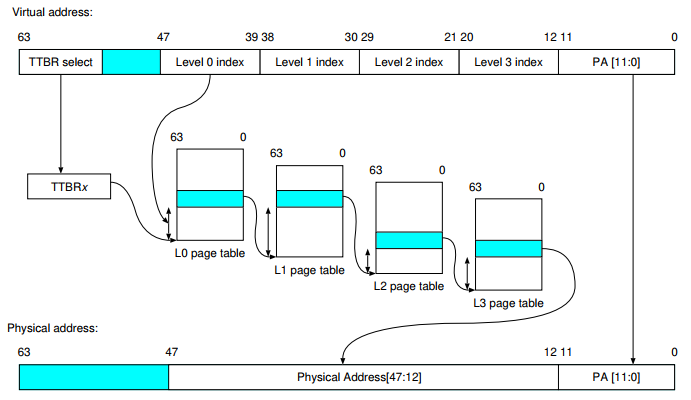
\includegraphics[scale=0.6]{images/memory/page_table.png}
    \caption{ARMv8-A page table with 4KB pages}
\end{figure}

\section{Page fault and lazy paging}

We can remark that storing page tables for all possible entries and levels would require $2^36$ * sizeof(entry) byte which would be way to much. A way to circumvent that is to specify for each level in each valid table if an entry is valid or not. If it is not valid, this means that the whole virtual memory range backed by this entry is not mapped so we do not have to store the underlying higher level page tables and entries.

In the event where we access a virtual memory address which is not backed by physical memory, during the physical address resolution, the index pointing to the next page table level or frame will be invalid. In this cause, an exception called page fault will be triggered. The Barrelfish micro-kernel catches this page fault and allows us to define a page fault handler which will be called in this case. The page fault handler can then be used to map physical memory at the virtual address location which triggered the page fault and then the process can resume as if nothing happened.

This allows us to use the concept of lazy paging: the virtual memory allocator can mark some memory pages as lazily allocated: there is not any physical memory backing it but as soon as we try to read or write from it, the page handler will in a transparent way map memory when necessary.
As such, if we lazily allocate 10GB of memory but only use 16MB of it, only 16MB of physical memory will get allocated and the process won't suffer from insufficient memory.



\section{Mapping Memory}

Apart from using a Red-Black Tree to handle the virtual address space, as explained earlier, it is crucial for us to monitor and consistently update the mappings to the \emph{physical address space}.

In our implementation, we opted to keep track of a process' mappings in a data structure closely resembling a \href{https://en.wikipedia.org/wiki/Shadow_table}{Shadow Page Table}, as shown in Listing \ref{listing:shadow_pt}. As part of our \texttt{paging\_state}, we thus keep track of the \emph{root level} page table.

Whenever we update a process' virtual address translation via the MMU, we update our internal mapping correspondingly. This ensure that the Shadow Page Table is kept up to date throughout any mapping/unmapping performed as part of \texttt{paging.c}.

\begin{lstlisting}[caption={\texttt{page\_table}: Keeping Track of Memory Mappings},label={listing:shadow_pt}]
struct page_table {
   enum objtype type;           ///< type of the page table
   uint16_t index;              ///< index in the parent page table 
   struct capref page_table;    ///< page table capability
   struct capref mapping;       ///< mapping capability

   /// entries within the page table
   union page_table_entry {
       struct page_table *pt;   ///< if type != L3
       struct capref frame_cap; ///< if type == L3 (mapping)
   } entries[VMSAv8_64_PTABLE_NUM_ENTRIES];
   
   /// "bit-array" indicating lazy allocation (if type == L3)
   int32_t lazy[(VMSAv8_64_PTABLE_NUM_ENTRIES + 32 - 1) / 32];
   
   ///counts the number of non-NULL children
   uint16_t num_children;
};
\end{lstlisting}

We chose this particular data structure because it strikes an excellent balance between efficiency and simplicity. Since nearly all upcoming milestones rely on the functionality provided in paging.c, it is imperative that we ensure its efficiency, reliability, and ease of debugging. Looking back, this decision has turned out to be incredibly valuable. During our development process, we encountered intricate bugs within our paging implementation that would have been significantly more challenging to debug if we had chosen a more complex data structure.


\subsection{Mapping a Frame}

We must provide the following functions to map a frame:
\begin{lstlisting}[caption={Mapping a Frame}]
errval_t paging_map_frame_attr_offset(struct paging_state *st, void **buf, size_t bytes, struct capref frame, size_t offset, int flags);

errval_t paging_map_fixed_attr_offset(struct paging_state *st, lvaddr_t vaddr, struct capref frame, size_t bytes, size_t offset, int flags);
\end{lstlisting}

Both functions are conceptually very similar. For \texttt{paging\_map\_frame\_attr\_offset} we may map the frame to any virtual address, where as the caller explicitly provides a desired virtual address as part of \texttt{paging\_map\_fixed\_attr\_offset}.

Our implementation reflects the similarity between the two functions. In both cases, we first perform the corresponding function to allocate the required virtual address space. Subsequently, we traverse our Shadow Page Table, allocating and initializing any child (shadow) page tables, if required.

In cases where mappings extend across multiple pages, we can easily handle them by iterating over the address space and mapping the frame with the appropriate offset. However, if the span of the mapping fits within a single leaf page table, we can avoid repeating the process of traversing the entire recursive mapping. It is worth noting that, in line with our objective of facilitating efficient debugging, we made a deliberate decision not to explicitly handle these specific edge cases, instead we always traverse the entire root to leaf mapping.

For the purpose of lazy allocations, we additionally support:
\begin{lstlisting}[caption={Mapping a Frame (Lazy)}]
    errval_t try_map(struct paging_state *st, lvaddr_t vaddr);
\end{lstlisting}
In particular, \texttt{try\_map} does not map the entire region, instead the mapping is performed lazily in this case. Here, we look up the virtual address allocation containing the provided \texttt{vaddr}, and make sure to map it. Furthermore, we make sure to set the corresponding bit in the \texttt{lazy} bit-array, as captured in Listing \ref{listing:shadow_pt}. This ensures that we can perform the necessary steps for lazily allocated regions during unmapping. 

\subsection{Unmapping a Frame}

\texttt{paging\_unmap} is used to unmap a previously mapped frame:
\begin{lstlisting}[caption={Unmapping a Frame}]
    errval_t paging_unmap(struct paging_state *st, 
                          const void *region);
\end{lstlisting}

Unmapping frames is conceptually very similar to mapping them. We find the virtual address region belonging to the provided \texttt{region} pointer, and then traverse our Shadow Page Table undoing any previously performed mappings. At the leaf level, we make use of the previously introduced \texttt{lazy} bitset. If the corresponding frame was allocated lazily, we make sure to also \texttt{cap\_destory} the corresponding frame. Finally, we free the corresponding allocation in the virtual address space. Once again the unmapping of regions spanning multiple pages is done by iterating over every contained page.

We additionally provide
\begin{lstlisting}[caption={Mapping a Frame}]
errval_t paging_decommit(struct paging_state *st, lvaddr_t vaddr, size_t bytes);
\end{lstlisting}
for the purpose of unmapping the corresponding region, while preserving the allocation in the virtual address space.

\subsection{Handling a Page Fault}

There are two main components that can be adjusted to decide how a page fault will be handled.

The first of these is the exception handler stack. While it may seem that the simplest solution would be to simply continue using the same stack when an exception occurs, this solution has a significant fault: Each thread's stack is also dynamically allocated, and not fully backed by memory. This means that, if the exception handler used the same stack as the rest of the program, it might run into a page fault while handling a page fault (which would terminate the execution of the program). Instead, we maintain a slab allocator which manages smaller, but fully mapped, slabs of memory to use as exception handler stacks. When a thread is created, its exception handler stack is allocated from this pool. This guarantees that no exceptions occur while handling an exception.

The second is the actual page fault handler function, which is called \texttt{\_paging\_handle\_exception} in our implementation. The function is conceptually very simple:
When a page fault occurs, we identify the associated virtual address space allocation and proceed to map it using the \texttt{try\_map} function, ensuring there is adequate space available in the slab allocator.

To facilitate more precise debugging, we deliberately trigger a panic if we encounter any address resolution within the first \texttt{BASE\_PAGE\_SIZE} bytes, as this usually implies a \texttt{NULL} pointer dereference.

Both the handler function and the exception handler stack are set up before a thread begins executing its target function.

\begin{comment}
We talked only about using 4KB pages. However, there are different page sizes available. For example, we could store directly a frame in a L2 page table entry. The frame will then be a 2MB page. We did not implement huge pages in our OS.
\end{comment}

\begin{comment}


Virtual memory manager

Allocating virtual memory

Different class of allocators

Red black trees

Paging

Why paging
Currently we have two memory managers. The first one is responsible for distributing physical memory (ram capabilities) to each process according to its needs. Once a process no longer needs memory, it can give it back and be used by another process. As far as virtual addressing is concerned, i.e. the address that the process sees, we have an ad-hoc memory allocator. However, there is still an open question. How to connect the virtual addresses to the physical addresses that represent the addresses in the ram. In order to solve this problem, we need a mechanism to translate in some way a virtual address into a physical adress. There is a technique to solve this problem. This technique is named paging.

What is paging exactly ?
Paging is a technique to translate a virtual address into a physical address. The processor maintains a data structure called a page table which will allow him to translate each virtual address into a physical one. When the processor reads a virtual address, it translates it and then reads the contents in memory of the translated physical address.

How does it work.

TODO : Add figure here

How did we implement it

How to implement it in practice

Memory request for a process:
When a processor needs memory, the operating system will request the virtual address. Our operating system will then request a physical address segment in the background and modify the page table data structure to translate the virtual addresses returned to the physical addresses returned by the allocator. To do this, we have two mechanisms to do it. The first is called eager allocation and the second is called lazy allocation.
The eager allocation works as follows. The operating system requests physical memory. It then requests virtual memory and directly builds the corresponding entries in the table entry page. This is the method used in our page_attr_offset function (todo: give good function name). If we assume that the page table will never be modified, we have by definition no page fault in the system. All the overhead of the installation is done at memory allocation time.
// TODO MAKE A SMALL SCHEME eager mapping
Lazy allocation works differently. When the process requests memory, the operating systems will ask the physical memory manager for a frame of the corresponding size and a segment in the virtual address. The operating systems does nothing else for the moment. Each time the program tries to translate and the page is not present, it will trigger an interrupt that corresponds to the page fault. At this point, the operating will perform the mapping "on the fly".

\end{comment}


\section{Virtual memory allocator}

\subsection{Role of the virtual memory allocator}

At this moment, we have the infrastructure to map and unmap pages, which allows us to bind the virtual address space to the physical addresses provided by our system and the capabilities. This is an essential step in the overall process, but it is only half of the work done.

Let's imagine we have the code that starts, stops, ends, and resumes a process. However, there is still an important question to answer: when should each process be allowed to run and for how long? This is known as a scheduling problem. In simpler terms, even though we know how to perform the mapping process, we haven't decided which specific mappings should happen. The only difference is that, instead of dividing computing power, we need to divide memory resources.

To grasp the concept better, let's consider a scenario where we have a group of tasks waiting to be executed. Each task requires a certain amount of resources, and we have a limited supply of these resources. It becomes essential to \texttt{prioritize} and \texttt{schedule} the tasks effectively to ensure \texttt{optimal resource utilization}.

In a similar manner, when dealing with mapping and unmapping pages in virtual memory, we encounter a similar challenge. We have a pool of virtual addresses and a finite set of physical addresses available for mapping. Our goal is to \texttt{efficiently allocate} these physical addresses to the virtual addresses in a way that maximizes the overall performance and resource utilization of our system.

To accomplish this, we need to develop a strategy or algorithm that determines the most effective mapping sequence. This algorithm would consider various factors, such as the size of the virtual address space, the available physical memory, the priority of the tasks, and any constraints or requirements imposed by the system.

Therefore, while we have the technical capability to perform the mapping and unmapping of pages, the larger task at hand is to devise an intelligent and efficient approach for deciding which specific mappings should be executed in what order. This ensures that the virtual address space is effectively connected to the physical addresses, optimizing the performance and resource management of the system as a whole.

\subsubsection{The choice of the memory allocator}

The task of managing virtual memory allocation is quite similar to managing physical memory allocation. In both cases, we have a set of addresses that we need to assign and release when they are no longer needed. There are various methods to implement a memory allocator, each using different algorithms. However, to simplify the process, we have two choices to consider.

One option is to start by implementing a simple allocator using a \texttt{linked list}. This approach would be easier to implement compared to more complex algorithms. With this allocator, inserting and freeing memory can be straightforward in the best-case scenario. However, as the number of allocated nodes increases, the operations become linear in nature. In other words, the performance of the system gradually decreases with multiple allocations, which is not an optimal outcome.

While the \texttt{linked list allocator} may be easy to implement initially, its performance shortcomings make it less ideal in the long run. It becomes apparent that a different approach is needed to achieve optimal memory allocation.

To address this limitation, we can explore other advanced algorithms such as \href{https://en.wikipedia.org/wiki/Binary_tree}{\texttt{binary trees}}, \href{https://www.cs.auckland.ac.nz/software/AlgAnim/red_black.html}{\texttt{red-black trees}}, or \href{https://en.wikipedia.org/wiki/Hash_table}{\texttt{hash tables}}. These data structures offer more efficient ways of managing memory allocation. For instance, binary trees enable faster search operations, while \texttt{red-black trees} provide a \texttt{balanced structure} that ensures efficient insertion and deletion operations. Hash tables, on the other hand, offer constant-time access to memory blocks, making them highly efficient.

By implementing one of these more advanced memory allocators, we can overcome the limitations of a simple linked list approach. These algorithms allow for improved performance even with multiple allocations, ensuring that the system operates at an optimal speed and efficiency.

After considering various options, we have chosen to implement a \texttt{red-black tree} for our memory allocator. This algorithm is more complicated to write and has a higher risk of bugs compared to a simple linked list. However, when it comes to performance, the \texttt{red-black tree} outshines the \texttt{linked list allocator}.

The key advantage of using a \texttt{red-black tree} is that its running time is \texttt{logarithmic}. This means that as the number of allocated nodes increases, the time it takes to perform operations like insertion and deletion grows much slower compared to a linearly increasing time in a \texttt{linked list}. In simpler terms, the \texttt{red-black tree} allows us to allocate and free memory blocks efficiently, resulting in faster processing overall.

In practical terms, implementing the \texttt{red-black tree} allocator means that our system will experience less overhead in memory allocation over time. This is because the performance of the \texttt{red-black tree} remains stable even as the number of allocated nodes grows. As a result, processes relying on memory allocation will suffer less from the associated delays and inefficiencies, leading to smoother and faster execution.

Although the \texttt{red-black tree allocator} requires more effort to implement and carries a higher risk of bugs, the long-term benefits in terms of performance make it a worthwhile choice. The trade-off between complexity and efficiency is justified by the significant improvement in running time and reduced overhead experienced by the system as a whole.

\subsubsection{The implementation of the red-black tree}

Each node in the tree represents a virtual memory range which can be used or free and they are ordered using their virtual memory range, as they don't overlap. Using a balanced binary tree allows us to do the following operations in \texttt{worst-case logarithmic time}:

\begin{itemize}
    \item \verb|Insert|(T, u): Insert node u in the tree T, effectively adding a new memory range to the tree
    \item \verb|Remove|(T,u): Remove node u from tree T, removing a managed range from the tree
    \item \verb|Pred|(T,u): Find the memory range before the one managed by u
    \item \verb|Succ|(T,u): Find the memory range after the one managed by u
    \item \verb|Find|(T, r): Find the memory range containing the virtual address r
\end{itemize}


\begin{lstlisting}[caption={The red-black tree node},label={listing:shadow_pt}]
/// @brief A node in the red-black tree, if in the tree, its fields should only be read
/// The field start can be modified given that it does not modify the node position relative
/// to the other nodes. The field size should only be modified using the rb_tree_update_size method
/// The max_size field is automatically maintained
struct rb_node {
    struct rb_node *parent;
    struct rb_node *left;
    struct rb_node *right;

    lvaddr_t start;
    size_t   size;

    size_t max_size;
    bool   is_red;
};

/// @brief An augmented red-back tree
struct rb_tree {
    struct rb_node *root;
};
\end{lstlisting}


\begin{lstlisting}[caption={Functions availables in the red-black tree},label={listing:shadow_pt}]
// Initialize the red-black tree, call before using the tree for the first time
void rb_tree_init(struct rb_tree *tree);

// Insert a node in the tree
// z should have been externally allocated and have its start and size fields already set
void rb_tree_insert(struct rb_tree *tree, struct rb_node *z);

// Remove a node from the tree
// z should point to a node already in the tree
void rb_tree_delete(struct rb_tree *tree, struct rb_node *z);

// Return the node containing the given address or NULL if none was found
struct rb_node *rb_tree_find(struct rb_tree *tree, lvaddr_t addr);

// Return a node of size at least size or NULL if none exists
// A worst-fit strategy is used
struct rb_node *rb_tree_find_minsize(struct rb_tree *tree, size_t size);

// return the first node wich starts at an addres greater or equal to addr
// or NULL if no such node exists
struct rb_node *rb_tree_find_greater(struct rb_tree *tree, lvaddr_t addr);

// return the first node wich starts at an addres lower or equal to addr
// or NULL if no such node exists
struct rb_node *rb_tree_find_lower(struct rb_tree *tree, lvaddr_t addr);

struct rb_node *rb_tree_successor(struct rb_node *node);

struct rb_node *rb_tree_predecessor(struct rb_node *node);

// Update the size of a node, without having to remove and re-insert it
void rb_tree_update_size(struct rb_node *node, size_t size);

// Helper function to check if a tree was corrupted
// Return true if the tree is fine
bool rb_tree_check(struct rb_tree *tree);

// Print the content of the tree using debug_printf
// The nodes are printed using an inorder walk
void rb_tree_print(struct rb_tree *tree);

\end{lstlisting}

Moreover, the tree is augmented with a \verb|size| attribute. This field gives for each node the size of the largest contiguous free virtual range in the subtree rooted at this node. Using this, we can immediately know for a given size if there is enough contiguous space to map it and makes implementing a worst-fit strategy for the memory allocation really easy. This data structure can also be used to allocate at a fixed location or tell that it is not possible.

\section{Morecore implementation}

The \texttt{malloc} function used to dynamically allocate memory internally calls a \verb|morecore| function when it requires more memory. We want the memory returned by multiple calls to morecore to be as often as possible contiguous to decrease fragmentation when alternating between malloc and free. This is a perfect use case for the lazy paging approach.

When morecore gets called, a 256GB contiguous memory range gets reserved, then we use a linear allocator in it to return memory. Thanks to lazy paging, only the range that gets used will actually be physically backed by memory and doing so, we reduce fragmentation. There are of course special cases if we malloc more than 256GB of memory at once (just reserve a memory range that is big enough) or overall more than 256GB (reserve a new 256GB memory range and switch to it).

\section{Retrospective}

When we look at how important the virtual memory allocator is in Barrelfish, just like its physical memory allocator counterpart, the most important thing is that it works reliably. Any mistake can (and did) lead to hard-to-debug issues later. 

In terms performance, our virtual memory allocator has shown less problems over time compared to the physical memory allocator. This is expected, as it uses a data structure with logarithmic time complexity, while the physical memory allocator has linear complexity in the worst case.

\chapter[Processes]{Processes \\ \Large \textnormal{Group Milestone}}

\section{Introduction}

In computer science, a \href{https://en.wikipedia.org/wiki/Process_(computing)}{\texttt{process}} refers to an instance of a computer program that is being executed. It represents the \texttt{running state} of a program along with its associated \texttt{resources}, such as memory, files, and input/output devices. A process is an \texttt{isolated entity} with its own address space, allowing it to operate independently of other processes. It is managed by the operating system, which schedules and allocates resources to processes, ensuring their proper execution and coordination within the system. In other words, process are a \texttt{virtualization mechanism} for the cpu.

Our operating system can only run a simple process for the moment. It is time to extend it so that it is able to run several processes in parallel. The first part explains the creation of a process and the subtleties. The second part talks about \texttt{process management}. Once an operating system has several processes, there are two questions that become central. The first one is how to divide the computing power (cycles in the processors) between the different processes that are executed. The second is how to manage the whole process life cycle. Launching it is certainly an important step, but it must be possible to stop it and eventually resume it later. Once finished, you also have to clean up the resources. Below is an illustration of the complexity of this problem and the UNIX solution. 

\subsection{Technical words and concepts used in this section}

\subsubsection{Dispatcher}

The \texttt{Barrelfish CPU driver} utilizes a \texttt{capability} type known as a \texttt{dispatcher control block (DCB)} to encapsulate all relevant information about a process assigned to a specific core (dispatcher). When a process is spawned, it creates a\texttt{DCB} and subsequently provides it to the \texttt{CPU driver}. This designated memory area serves as a storage for various details pertaining to the process. For instance, it holds information such as the register state during a \texttt{context switch} and the error handlers to be invoked in the event of page faults.

\subsubsection{Elf image}

An \texttt{ELF (Executable and Linkable Format)} image refers to a common file format used for \texttt{executable files}, \texttt{object code} and \texttt{shared libraries} in many Unix-like operating systems. It serves as a \texttt{standardized} format for representing binary files that can be executed directly by a computer's processor or linked with other modules during the compilation and building process.

ELF images typically contain the compiled machine code, data, and other necessary information for an executable program or shared library. They consist of several sections, such as the program header table, which provides details about the layout and memory requirements of the executable, and the section header table, which defines individual sections containing different types of data (e.g., code, data, symbols, etc.).

\section{Starting a new process}

The process of initiating a a new process involves a series of sequential steps that need to be carried out. Initially, we embark upon the task of loading our elf binary into the memory. Following that, we proceed with establishing the \texttt{capability space}, ensuring that it is properly configured and ready for use. In the subsequent phase, we set up the \texttt{virtual address space}, ensuring that the necessary mappings and translations are in place inside of the page tables entries. Moving forward, we engage in the process of \texttt{parsing} our \texttt{binary image}, meticulously extracting the relevant information and structuring it appropriately. This part was very tricky and with a lot of subtleties. Subsequently, we set up the dispatcher and configure it by filling various fiend inside of the structure. Only once each of these steps has been successfully executed, are we able to \texttt{invoke} the dispatcher, initiating in the operation system the newly created process.

\subsection{Setup the capability space}

A process cannot generate something out of nothing; that would be considered magical. It requires a specific amount of RAM and certain abilities to effectively handle its virtual address space. To achieve this, we generate multiple capabilities, each with its own designated function.

The procedure for creating a capability is as follows: Initially, we must generate a capability within the parent process (for instance, a RAM-type capability). Next, we assign an address within the child's capability space. The final step involves \texttt{transferring} the capability from the parent to the child. The provided example illustrates how this is accomplished in the context of Barrelfish.


\begin{lstlisting}[caption={Typical process of creation and mapping of capability},language=C,frame=single,breaklines]
struct capref physical_chunk;
size_t        frame_size = 1024 * 1024;

err = ram_alloc(&physical_chunk, frame_size);
if (err_is_fail(err)) {
    return err_push(err, LIB_ERR_FRAME_ALLOC);
}

struct capref earlymem_capref = {
    .cnode = *rootcn_slot_taskcn,
    .slot  = TASKCN_SLOT_EARLYMEM,
};

err = cap_copy(earlymem_capref, physical_chunk);
if (err_is_fail(err)) {
    return err_push(err, LIB_ERR_CAP_COPY);
}
\end{lstlisting}

We have several capabilities that require mapping. Firstly, we need a self-capability for inter-core communication purposes. Additionally, we require a capability for the dispatcher, another one for the root L1 node, and one for the dispatcher frame. We also have the command line arguments that need to be mapped, as well as a capability for memory allocations. It's important to note that we don't need to pass a capability for devices, as all drivers reside in the initialization phase. This is however specific to our operating system. Lastly, we need to map multiple-level C2 nodes for the slot allocator and the page tables.
\subsection{Setup the virtual address space}

We have received a slot that we can use to allocate the core that represents level 0 of the page table. First we allocate a capability with the allocator slot and create an object of type \texttt{ObjType\_VNode\_AARCH64\_l0} which corresponds to our level 0 in the page table (the root page table). Once this part is executed, we can use cap copy to copy the content to the address space of the child. Once we have done these steps, we can initialize the paging structure with \texttt{paging\_init\_state\_foreign}. 

\subsection{Parse the elf image}

The next step is to convert the ELF binary image into an object that can be executed. In this conversion we need to perform several operations. The first thing is to load the binary image into memory. There is a part that we need to pay attention to. We load from the parent process, but we will use from the child process. This means that we have to actually map the virtual addressing in the two address spaces and in each case to a different value.

We had a bug that took us a really long time to fix and it was relatively tricky. Indeed we can give flags to different pages. This means that we can for example read and write or just read. When we are in the parent process, we want to be able to manipulate the pages and therefore should have all rights by default. This is the reason why we make a map with the two following flags \texttt{VREGION\_FLAGS\_READ | VREGION\_FLAGS\_WRITE}. 

Once we have loaded the program into memory, we can retrieve the key values we need for the next step, such as the global offset table.

\subsection{Setup the arguments}

The next step is to move the arguments from the \texttt{parent process} to the \texttt{child process}. This step allows to launch the main function of the process with argc and argv[]. This part was not the hardest in terms of absolute difficulty, but we had to be careful because we were working and copying in two different \texttt{virtual address spaces}. Indeed we copy the arguments from the parent's process (and thus from the parent's virtual addressing) and we have to give a pointer in virtual addressing in the child's process. This implies that we have to give another virtual address and the calculation of the offset is done in the following way. Below we can see the formula for the translation:
\begin{equation*}
    \texttt{start\_address} - \texttt{parent\_vaddr\_to\_physical} + \texttt{child\_vaddr\_to\_physical}
\end{equation*}

\subsection{Setting up the dispatcher}

The \texttt{Barrelfish CPU driver} employs a \texttt{capability} type known as a \texttt{dispatcher control block (DCB)} to encompass all relevant details of a process. The spawning process generates the \texttt{DCB} and subsequently transfers it to the \texttt{CPU driver}. This designated region of memory is utilized by the \texttt{CPU driver} to store information pertaining to the process, e.g., the register state during a context switch, and the process' error handlers.

We set up the \texttt{DCB} following the guidelines and instructions provided in the relevant section of the AOS Book. First, we allocate a frame and map it into both the address space of the parent as well as the address space of the parent. Subsequently, we populate the frame with the relevant information. This includes, setting up the entry point, the base address of the global offset table, and the pointer to the child's command line arguments. Finally, we must take care to store the allocated frame, i.e., the \texttt{DCB}, in the appropriate slot within the child's CSpace (\texttt{TASKCN\_SLOT\_DISPFRAME}).

\subsection{Invoking the dispatcher}

After ensuring that all the necessary preparations are in place, we are able to proceed with invoking the dispatcher function, which serves the purpose of arranging and coordinating the process within the operating system. Upon reaching this stage, we find ourselves in possession of an operating system endowed with the capability to concurrently handle and execute two distinct processes.

\begin{lstlisting}[caption={The structure holding a single process},language=C,frame=single,breaklines]
struct spawninfo {
    /// name of the binary this process runs
    char *binary_name;

    /// the full commandline of this process, including its arguments
    char *cmdline;

    /// PID of this process
    domainid_t pid;

    /// execution state of this process
    spawn_state_t state;

    /// exit code of this process, or zero if it hasn't exited yet
    int exitcode;

    // RPC server for the child process
    struct aos_rpc rpc_server;

    // L1 Cnode used for the child process
    struct capref cspace;
    // L0 page table used for the child process
    struct capref vspace;

    // Dispatcher associated with the child process
    struct capref dispatcher;

    /// Amount of bytes in memory that has been granted
    size_t mem;
};
\end{lstlisting}

\section{Scheduling and managing processes}

\subsection{Life of a process}

Unlike traditional \href{https://en.wikipedia.org/wiki/Unix-like}{\texttt{UNIX-style operating systems}} that have complex process \texttt{lifecycles} with many states, our operating system takes a simpler approach. We have a total of 6 different states called spawn\_load, spawn\_start, spawn\_pause, spawn\_resume, spawn\_killed, and spawn\_exit. Here is a list of all the states we have in our operating system:

\begin{itemize}
    \item \textbf{spawn\_load}: This initial state denotes the loading phase of a process, where the necessary resources and data are being allocated and initialized to prepare for execution.

    \item \textbf{spawn\_start}: Once the loading phase is complete, the process transitions to the spawn\_start state. Here, the process is launched and commences its execution, performing the intended tasks.

    \item \textbf{spawn\_pause}: In certain scenarios, it may be necessary to temporarily halt the execution of a process. The spawn\_pause state represents such a pause, where the process is temporarily suspended, preserving its current state until it is resumed.

    \item \textbf{spawn\_resume}: When a process in the spawn\_pause state is ready to resume its execution, it transitions to the spawn\_resume state. Here, the process recommences its tasks from where it left off, continuing its intended operations.

    \item \textbf{spawn\_killed}: Under specific circumstances, it may become necessary to terminate a process abruptly. The spawn\_killed state signifies such an event, where the process is forcefully terminated, terminating its execution and releasing associated resources.

    \item \textbf{spawn\_exit}: Finally, when a process completes its intended tasks or is terminated gracefully, it enters the spawn\_exit state. Here, the process wraps up its execution, performs necessary clean-up activities, and releases any acquired resources before concluding its lifecycle.
\end{itemize}

\begin{comment}
\begin{figure}[htp]
    \centering
    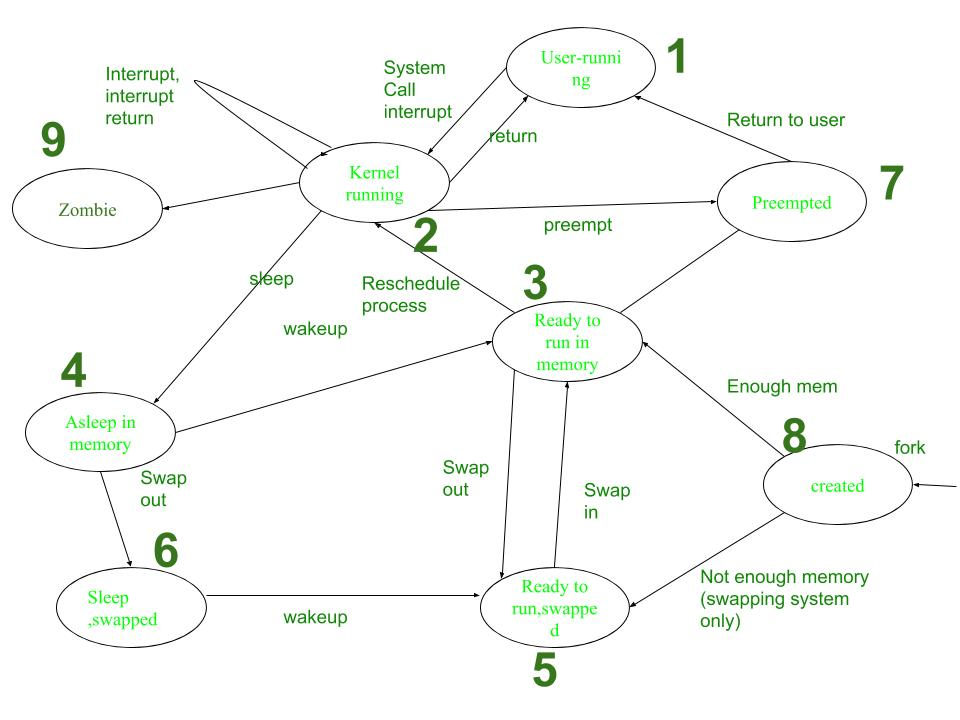
\includegraphics[width=12cm]{images/process/process.jpeg}
    \setcaptioncitation{https://www.geeksforgeeks.org/process-states-and-transitions-in-a-unix-process}
    \caption{Process life cycle in a typical unix system}
    \label{fig:galaxy}
\end{figure}
\end{comment}




\begin{figure}[htp]
    \centering
\tikzset{every picture/.style={line width=0.75pt}} %set default line width to 0.75pt        

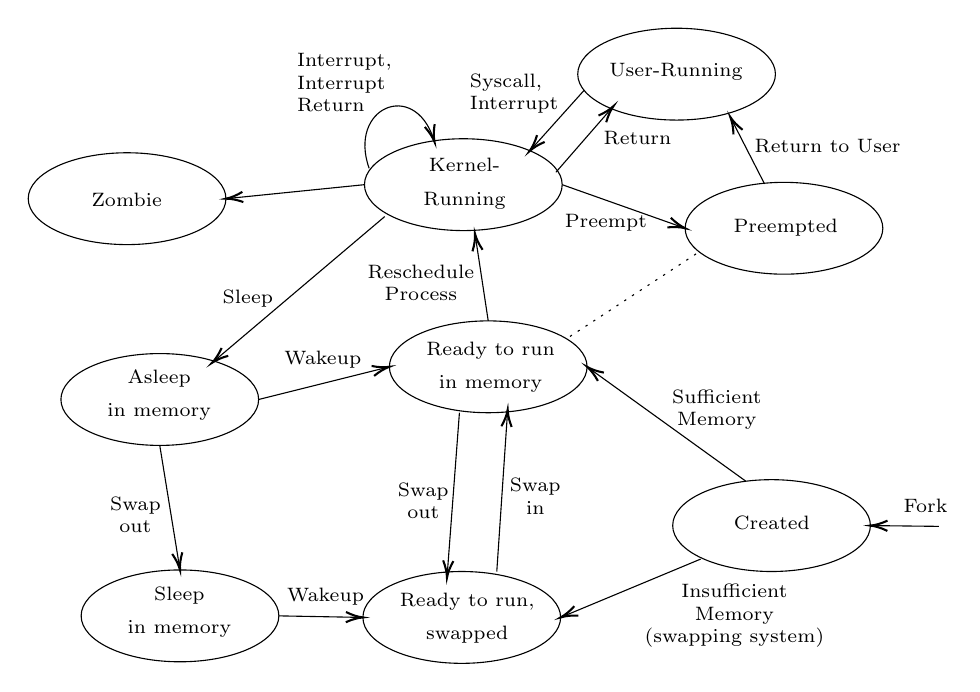
\begin{tikzpicture}[x=0.75pt,y=0.75pt,yscale=-0.75,xscale=0.75]
%uncomment if require: \path (0,505); %set diagram left start at 0, and has height of 505

%Flowchart: Connector [id:dp8160970570643812] 
\draw   (267,248.5) .. controls (267,232.21) and (295.43,219) .. (330.5,219) .. controls (365.57,219) and (394,232.21) .. (394,248.5) .. controls (394,264.79) and (365.57,278) .. (330.5,278) .. controls (295.43,278) and (267,264.79) .. (267,248.5) -- cycle ;
%Flowchart: Connector [id:dp07062083514363515] 
\draw   (457,159.5) .. controls (457,143.21) and (485.43,130) .. (520.5,130) .. controls (555.57,130) and (584,143.21) .. (584,159.5) .. controls (584,175.79) and (555.57,189) .. (520.5,189) .. controls (485.43,189) and (457,175.79) .. (457,159.5) -- cycle ;
%Flowchart: Connector [id:dp18553524714572012] 
\draw   (388,60.5) .. controls (388,44.21) and (416.43,31) .. (451.5,31) .. controls (486.57,31) and (515,44.21) .. (515,60.5) .. controls (515,76.79) and (486.57,90) .. (451.5,90) .. controls (416.43,90) and (388,76.79) .. (388,60.5) -- cycle ;
%Flowchart: Connector [id:dp7880945062151502] 
\draw   (449,350.5) .. controls (449,334.21) and (477.43,321) .. (512.5,321) .. controls (547.57,321) and (576,334.21) .. (576,350.5) .. controls (576,366.79) and (547.57,380) .. (512.5,380) .. controls (477.43,380) and (449,366.79) .. (449,350.5) -- cycle ;
%Flowchart: Connector [id:dp07153592237662654] 
\draw   (250,409.5) .. controls (250,393.21) and (278.43,380) .. (313.5,380) .. controls (348.57,380) and (377,393.21) .. (377,409.5) .. controls (377,425.79) and (348.57,439) .. (313.5,439) .. controls (278.43,439) and (250,425.79) .. (250,409.5) -- cycle ;
%Flowchart: Connector [id:dp8290378636635095] 
\draw   (251,131.5) .. controls (251,115.21) and (279.43,102) .. (314.5,102) .. controls (349.57,102) and (378,115.21) .. (378,131.5) .. controls (378,147.79) and (349.57,161) .. (314.5,161) .. controls (279.43,161) and (251,147.79) .. (251,131.5) -- cycle ;
%Flowchart: Connector [id:dp6001380034764758] 
\draw   (35,140.5) .. controls (35,124.21) and (63.43,111) .. (98.5,111) .. controls (133.57,111) and (162,124.21) .. (162,140.5) .. controls (162,156.79) and (133.57,170) .. (98.5,170) .. controls (63.43,170) and (35,156.79) .. (35,140.5) -- cycle ;
%Flowchart: Connector [id:dp3608424050702036] 
\draw   (56,269.5) .. controls (56,253.21) and (84.43,240) .. (119.5,240) .. controls (154.57,240) and (183,253.21) .. (183,269.5) .. controls (183,285.79) and (154.57,299) .. (119.5,299) .. controls (84.43,299) and (56,285.79) .. (56,269.5) -- cycle ;
%Flowchart: Connector [id:dp1472588739314128] 
\draw   (69,408.5) .. controls (69,392.21) and (97.43,379) .. (132.5,379) .. controls (167.57,379) and (196,392.21) .. (196,408.5) .. controls (196,424.79) and (167.57,438) .. (132.5,438) .. controls (97.43,438) and (69,424.79) .. (69,408.5) -- cycle ;
%Curve Lines [id:da24258380703786953] 
\draw    (254,121) .. controls (240.21,82.12) and (282.69,63.56) .. (295.44,102.2) ;
\draw [shift={(296,104)}, rotate = 253.69] [color={rgb, 255:red, 0; green, 0; blue, 0 }  ][line width=0.75]    (10.93,-3.29) .. controls (6.95,-1.4) and (3.31,-0.3) .. (0,0) .. controls (3.31,0.3) and (6.95,1.4) .. (10.93,3.29)   ;
%Straight Lines [id:da7972175227854316] 
\draw    (251,131.5) -- (163.99,140.3) ;
\draw [shift={(162,140.5)}, rotate = 354.23] [color={rgb, 255:red, 0; green, 0; blue, 0 }  ][line width=0.75]    (10.93,-3.29) .. controls (6.95,-1.4) and (3.31,-0.3) .. (0,0) .. controls (3.31,0.3) and (6.95,1.4) .. (10.93,3.29)   ;
%Straight Lines [id:da14343662453882478] 
\draw    (264,152) -- (154.53,244.71) ;
\draw [shift={(153,246)}, rotate = 319.74] [color={rgb, 255:red, 0; green, 0; blue, 0 }  ][line width=0.75]    (10.93,-3.29) .. controls (6.95,-1.4) and (3.31,-0.3) .. (0,0) .. controls (3.31,0.3) and (6.95,1.4) .. (10.93,3.29)   ;
%Straight Lines [id:da7814144535871211] 
\draw    (119.5,299) -- (132.18,377.03) ;
\draw [shift={(132.5,379)}, rotate = 260.77] [color={rgb, 255:red, 0; green, 0; blue, 0 }  ][line width=0.75]    (10.93,-3.29) .. controls (6.95,-1.4) and (3.31,-0.3) .. (0,0) .. controls (3.31,0.3) and (6.95,1.4) .. (10.93,3.29)   ;
%Straight Lines [id:da22986834689597324] 
\draw    (196,408.5) -- (248,409.46) ;
\draw [shift={(250,409.5)}, rotate = 181.06] [color={rgb, 255:red, 0; green, 0; blue, 0 }  ][line width=0.75]    (10.93,-3.29) .. controls (6.95,-1.4) and (3.31,-0.3) .. (0,0) .. controls (3.31,0.3) and (6.95,1.4) .. (10.93,3.29)   ;
%Straight Lines [id:da5183246324311807] 
\draw    (183,269.5) -- (265.06,248.99) ;
\draw [shift={(267,248.5)}, rotate = 165.96] [color={rgb, 255:red, 0; green, 0; blue, 0 }  ][line width=0.75]    (10.93,-3.29) .. controls (6.95,-1.4) and (3.31,-0.3) .. (0,0) .. controls (3.31,0.3) and (6.95,1.4) .. (10.93,3.29)   ;
%Straight Lines [id:da36938160925280306] 
\draw    (312,278) -- (304.15,382.01) ;
\draw [shift={(304,384)}, rotate = 274.32] [color={rgb, 255:red, 0; green, 0; blue, 0 }  ][line width=0.75]    (10.93,-3.29) .. controls (6.95,-1.4) and (3.31,-0.3) .. (0,0) .. controls (3.31,0.3) and (6.95,1.4) .. (10.93,3.29)   ;
%Straight Lines [id:da1895995011282201] 
\draw    (336,380) -- (342.87,278) ;
\draw [shift={(343,276)}, rotate = 93.85] [color={rgb, 255:red, 0; green, 0; blue, 0 }  ][line width=0.75]    (10.93,-3.29) .. controls (6.95,-1.4) and (3.31,-0.3) .. (0,0) .. controls (3.31,0.3) and (6.95,1.4) .. (10.93,3.29)   ;
%Straight Lines [id:da5028228919093697] 
\draw    (467,372) -- (378.85,408.73) ;
\draw [shift={(377,409.5)}, rotate = 337.38] [color={rgb, 255:red, 0; green, 0; blue, 0 }  ][line width=0.75]    (10.93,-3.29) .. controls (6.95,-1.4) and (3.31,-0.3) .. (0,0) .. controls (3.31,0.3) and (6.95,1.4) .. (10.93,3.29)   ;
%Straight Lines [id:da15122238928340714] 
\draw    (496,322) -- (395.62,249.67) ;
\draw [shift={(394,248.5)}, rotate = 35.78] [color={rgb, 255:red, 0; green, 0; blue, 0 }  ][line width=0.75]    (10.93,-3.29) .. controls (6.95,-1.4) and (3.31,-0.3) .. (0,0) .. controls (3.31,0.3) and (6.95,1.4) .. (10.93,3.29)   ;
%Straight Lines [id:da9119462488777964] 
\draw  [dash pattern={on 0.84pt off 2.51pt}]  (464,176) -- (380,231) ;
%Straight Lines [id:da08612669312273191] 
\draw    (378,131.5) -- (455.11,158.83) ;
\draw [shift={(457,159.5)}, rotate = 199.52] [color={rgb, 255:red, 0; green, 0; blue, 0 }  ][line width=0.75]    (10.93,-3.29) .. controls (6.95,-1.4) and (3.31,-0.3) .. (0,0) .. controls (3.31,0.3) and (6.95,1.4) .. (10.93,3.29)   ;
%Straight Lines [id:da9129325725415524] 
\draw    (508,131) -- (486.91,89.78) ;
\draw [shift={(486,88)}, rotate = 62.9] [color={rgb, 255:red, 0; green, 0; blue, 0 }  ][line width=0.75]    (10.93,-3.29) .. controls (6.95,-1.4) and (3.31,-0.3) .. (0,0) .. controls (3.31,0.3) and (6.95,1.4) .. (10.93,3.29)   ;
%Straight Lines [id:da9605770765837162] 
\draw    (374,123.5) -- (409.69,82.51) ;
\draw [shift={(411,81)}, rotate = 131.04] [color={rgb, 255:red, 0; green, 0; blue, 0 }  ][line width=0.75]    (10.93,-3.29) .. controls (6.95,-1.4) and (3.31,-0.3) .. (0,0) .. controls (3.31,0.3) and (6.95,1.4) .. (10.93,3.29)   ;
%Straight Lines [id:da6816726572039686] 
\draw    (392,71) -- (358.34,108.51) ;
\draw [shift={(357,110)}, rotate = 311.91] [color={rgb, 255:red, 0; green, 0; blue, 0 }  ][line width=0.75]    (10.93,-3.29) .. controls (6.95,-1.4) and (3.31,-0.3) .. (0,0) .. controls (3.31,0.3) and (6.95,1.4) .. (10.93,3.29)   ;
%Straight Lines [id:da11655688316633739] 
\draw    (330.5,219) -- (322.3,164.98) ;
\draw [shift={(322,163)}, rotate = 81.37] [color={rgb, 255:red, 0; green, 0; blue, 0 }  ][line width=0.75]    (10.93,-3.29) .. controls (6.95,-1.4) and (3.31,-0.3) .. (0,0) .. controls (3.31,0.3) and (6.95,1.4) .. (10.93,3.29)   ;
%Straight Lines [id:da026693159156937374] 
\draw    (620,351) -- (578,350.52) ;
\draw [shift={(576,350.5)}, rotate = 0.65] [color={rgb, 255:red, 0; green, 0; blue, 0 }  ][line width=0.75]    (10.93,-3.29) .. controls (6.95,-1.4) and (3.31,-0.3) .. (0,0) .. controls (3.31,0.3) and (6.95,1.4) .. (10.93,3.29)   ;

% Text Node
\draw (277,231) node [anchor=north west][inner sep=0.75pt]  [font=\normalsize] [align=left] {\begin{minipage}[lt]{60pt}\setlength\topsep{0pt}
\begin{center}
{\scriptsize Ready to run \\ \scriptsize in memory}
\end{center}

\end{minipage}};
% Text Node
\draw (485,152) node [anchor=north west][inner sep=0.75pt]   [align=left] {\begin{minipage}[lt]{39.31pt}\setlength\topsep{0pt}
\begin{center}
{\scriptsize Preempted}
\end{center}

\end{minipage}};
% Text Node
\draw (406,52) node [anchor=north west][inner sep=0.75pt]   [align=left] {\begin{minipage}[lt]{48.88pt}\setlength\topsep{0pt}
\begin{center}
{\scriptsize User-Running}
\end{center}

\end{minipage}};
% Text Node
\draw (485,343) node [anchor=north west][inner sep=0.75pt]   [align=left] {\begin{minipage}[lt]{29.34pt}\setlength\topsep{0pt}
\begin{center}
{\scriptsize Created}
\end{center}

\end{minipage}};
% Text Node
\draw (262,392) node [anchor=north west][inner sep=0.75pt]   [align=left] {\begin{minipage}[lt]{60pt}\setlength\topsep{0pt}
\begin{center}
{\scriptsize Ready to run,}\\{\scriptsize swapped}
\end{center}

\end{minipage}};
% Text Node
\draw (265,113) node [anchor=north west][inner sep=0.75pt]   [align=left] {\begin{minipage}[lt]{54.7pt}\setlength\topsep{0pt}
\begin{center}
{\scriptsize Kernel-Running}
\end{center}

\end{minipage}};
% Text Node
\draw (72,135) node [anchor=north west][inner sep=0.75pt]   [align=left] {\begin{minipage}[lt]{27.67pt}\setlength\topsep{0pt}
\begin{center}
{\scriptsize Zombie}
\end{center}

\end{minipage}};
% Text Node
\draw (84,249) node [anchor=north west][inner sep=0.75pt]   [align=left] {\begin{minipage}[lt]{37.63pt}\setlength\topsep{0pt}
\begin{center}
{\scriptsize Asleep}\\{\scriptsize in memory}
\end{center}

\end{minipage}};
% Text Node
\draw (97,388) node [anchor=north west][inner sep=0.75pt]   [align=left] {\begin{minipage}[lt]{37.63pt}\setlength\topsep{0pt}
\begin{center}
{\scriptsize Sleep}\\{\scriptsize in memory}
\end{center}

\end{minipage}};
% Text Node
\draw (206,45.65) node [anchor=north west][inner sep=0.75pt]  [font=\scriptsize] [align=left] {Interrupt,\\Interrupt\\Return};
% Text Node
\draw (317,58.65) node [anchor=north west][inner sep=0.75pt]  [font=\scriptsize] [align=left] {Syscall,\\Interrupt};
% Text Node
\draw (403,95.65) node [anchor=north west][inner sep=0.75pt]  [font=\scriptsize] [align=left] {Return};
% Text Node
\draw (500,100.65) node [anchor=north west][inner sep=0.75pt]  [font=\scriptsize] [align=left] {Return to User};
% Text Node
\draw (378,149) node [anchor=north west][inner sep=0.75pt]  [font=\scriptsize] [align=left] {Preempt};
% Text Node
\draw (248,181.65) node [anchor=north west][inner sep=0.75pt]  [font=\scriptsize] [align=left] {\begin{minipage}[lt]{42.22pt}\setlength\topsep{0pt}
\begin{center}
Reschedule\\Process
\end{center}

\end{minipage}};
% Text Node
\draw (155,197.65) node [anchor=north west][inner sep=0.75pt]  [font=\scriptsize] [align=left] {\begin{minipage}[lt]{21.86pt}\setlength\topsep{0pt}
\begin{center}
Sleep
\end{center}

\end{minipage}};
% Text Node
\draw (196,237) node [anchor=north west][inner sep=0.75pt]  [font=\scriptsize] [align=left] {\begin{minipage}[lt]{29.89pt}\setlength\topsep{0pt}
\begin{center}
Wakeup
\end{center}

\end{minipage}};
% Text Node
\draw (72,330.65) node [anchor=north west][inner sep=0.75pt]  [font=\scriptsize] [align=left] {\begin{minipage}[lt]{33.92pt}\setlength\topsep{0pt}
\begin{center}
Swap\\out
\end{center}

\end{minipage}};
% Text Node
\draw (199,388.65) node [anchor=north west][inner sep=0.75pt]  [font=\scriptsize] [align=left] {\begin{minipage}[lt]{28.51pt}\setlength\topsep{0pt}
\begin{center}
Wakeup
\end{center}

\end{minipage}};
% Text Node
\draw (268,321.65) node [anchor=north west][inner sep=0.75pt]  [font=\scriptsize] [align=left] {\begin{minipage}[lt]{21.44pt}\setlength\topsep{0pt}
\begin{center}
Swap\\out
\end{center}

\end{minipage}};
% Text Node
\draw (340,318.65) node [anchor=north west][inner sep=0.75pt]  [font=\scriptsize] [align=left] {\begin{minipage}[lt]{21.44pt}\setlength\topsep{0pt}
\begin{center}
Swap\\in
\end{center}

\end{minipage}};
% Text Node
\draw (446,261.65) node [anchor=north west][inner sep=0.75pt]  [font=\scriptsize] [align=left] {\begin{minipage}[lt]{33.36pt}\setlength\topsep{0pt}
\begin{center}
Sufficient\\Memory
\end{center}

\end{minipage}};
% Text Node
\draw (427,386.65) node [anchor=north west][inner sep=0.75pt]  [font=\scriptsize] [align=left] {\begin{minipage}[lt]{67.44pt}\setlength\topsep{0pt}
\begin{center}
Insufficient Memory\\(swapping system)
\end{center}

\end{minipage}};
% Text Node
\draw (594,332) node [anchor=north west][inner sep=0.75pt]  [font=\scriptsize] [align=left] {\begin{minipage}[lt]{17.68pt}\setlength\topsep{0pt}
\begin{center}
Fork
\end{center}
\end{minipage}};
\end{tikzpicture}
    \caption[Process life cycle in a typical unix system]{Process life cycle in a typical unix system\footnotemark}
    \label{fig:galaxy}
\end{figure}
\footnotetext{Adapted from \href{https://www.geeksforgeeks.org/process-states-and-transitions-in-a-unix-process}{GeeksforGeeks: Process states and Transitions in a UNIX Process}}

\subsection{Process management}
In our operating system, the management of processes is entrusted to the \texttt{process manager}, a crucial component responsible for overseeing their execution. To facilitate this management, each core within the system maintains a linked list that encompasses comprehensive information about all the processes currently running.

This \href{https://en.wikipedia.org/wiki/Linked_list}{\texttt{linked list}} serves as a repository where data pertaining to various processes, such as their names and statuses, are stored. By traversing this list iteratively, we gain the ability to search for a specific process based on its given name. This search operation allows us to locate the desired process swiftly and efficiently, enabling us to access and modify its status as needed.

To ensure the uniqueness and identification of each process, a unique identifier, known as the \texttt{process ID (PID)}, is assigned to every process. This \texttt{PID} acts as a kind of \texttt{primary key}, distinguishing one process from another and facilitating their individual \texttt{identification} and management within the system.

\subsubsection{Process manager}

The process manager stores various pieces of information to effectively manage processes, including:

\begin{itemize}
    \item \textbf{Spawninfo}: The process manager stores spawninfo, which comprises essential details about the process, such as its initialization parameters, input/output channels, and other relevant configuration data.

    \item \textbf{LMP Channel}: In order to facilitate effective communication between the process and the system, the process manager maintains a dedicated LMP (Lightweight Message Passing) channel. This channel serves as a conduit through which messages can be exchanged between the process and other system components.

    \item \textbf{Process State}: The process manager keeps track of the state of each process. This information provides an indication of whether the process is actively executing, paused, terminated, or in any other state defined within the process lifecycle.

    \item \textbf{Exit Code}: Upon the completion or termination of a process, the process manager captures and stores the exit code. This code signifies the status or outcome of the process's execution and can be used for error handling or diagnostic purposes.

    \item \textbf{Linked List of Waiting Processes}: A function is available for a process to wait for another process to terminate. To do so, each process has a linked list containing all the processes that are awaiting its termination. Additionally, for each process in the waiting list, the process manager stores a callback function. These callbacks serve as notifications or actions that are triggered once the awaited process finishes its execution.
\end{itemize}


\subsubsection{Software pattern used to modify the state of a process}

In our system, we have various operations we can perform on processes, such as resuming a process, terminating a process, or finding the name of a process. Many of these functions follow a similar pattern. Below is an explanation:

To perform these operations, we rely on a data structure called \texttt{spawn info}. This structure contains important information about a process, including its current state. The first step in these functions is to search for the corresponding \texttt{spawn info} in the data structure. Once we find the \texttt{spawn info}, we can make the necessary modifications, such as changing the state of the process or performing other operations based on the specific function we are executing. This allows us to control the behavior of the process as needed.

To locate the relevant \texttt{spawn info}, we utilize a second routine. This routine iterates over a linked list that contains all the spawn info structures. It searches through the list to find the spawn info associated with the process we are working with. This ensures we have the correct information to perform the desired operation.

This pattern of searching for the spawn info and then applying the required modifications is similar to the concept of \href{https://cplusplus.com/reference/iterator/}{\texttt{iterators}} in C++. In C++, an iterator is an object that allows us to traverse through a \href{https://cplusplus.com/reference/stl/}{\texttt{container}} (in C++), such as a linked list, and access its elements one by one. Similarly, in our system, we iterate over the linked list to find the corresponding spawn info and make the necessary changes.


\begin{lstlisting}[caption={Data structures used for the process management},language=C,frame=single,breaklines]
// Linked list containing the processes waiting for a process to exit
struct proc_mgmt_exit_waiting_proc {
    struct event_closure                resume_fn;
    int                                *exit_code;
    struct proc_mgmt_exit_waiting_proc *next;
};

// Linked list containing all processes information
struct proc_mgmt_element {
    struct spawninfo         *si;
    struct proc_mgmt_exit_waiting_proc *waiting_procs;
    struct proc_mgmt_element *next;
};

// Process manager
struct proc_mgmt_state {
    // recursive mutex used for thread safety
    struct thread_mutex mutex;

    // Number of processes handled by this state
    size_t nb_processes_running;
    // list of all the processes handled
    struct proc_mgmt_element *procs;

    // next pid to be attributed
    domainid_t next_pid;
};
\end{lstlisting}

\begin{algorithm}
\caption{Iterate over process}
\begin{algorithmic}[1]

\Procedure{IterateOverProcesses}{\text{domainid\_t } \text{pid}, \text{void *} \text{parameters}}
\State $\text{err} \gets \text{check\_input()}$
\If{$\text{err\_fail}$}
    \Return $\text{INPUT\_ERROR}$
\EndIf

\State $\text{process\_management\_state} \gets \text{get\_process\_management\_state()}$
\State $\text{spawninfo} \gets \text{search\_process\_by\_pid}(\text{pms}, \text{pid})$

\If {$\text{spawninfo} = \text{NULL}$}
    \State \textbf{return} $\text{spawn\_domain\_not\_found}$
\EndIf

\State \text{apply\_specific\_operation\_on\_process()}
\State \textbf{return} $\text{SYS\_ERR\_OK}$
\EndProcedure

\end{algorithmic}
\end{algorithm}

\begin{algorithm}
\caption{Search process by pid}
\begin{algorithmic}[1]

\Procedure{SearchProcessByPID}{$\text{process\_management\_state, pid}$}

\State \Call{Lock()}{}
\State $\text{current\_process\_management\_element} \gets \text{process\_management\_state}\rightarrow \text{proccess\_management\_element}$


\While{$\text{current\_process\_management\_element} \neq \text{NULL}$}
    \If{$\text{current\_process\_management\_element}\rightarrow \text{pid} = \text{pid}$}
        \State \Call{Unlock()}{}
        \State \textbf{return} $\text{current\_process\_management\_element}\rightarrow \text{si}$
    \EndIf
    \State $\text{current\_process\_management\_element} \gets \text{current\_process\_management\_element}\rightarrow \text{next}$
\EndWhile


\State \Call{Unlock()}{}
\EndProcedure

\end{algorithmic}
\end{algorithm}

\subsubsection{Multicore management}

Managing processes on a \texttt{multicore system} is more intricate compared to a single-core system. It requires an efficient approach to gather resources and direct requests to the appropriate destinations. In a multicore setup, each core has its \texttt{own process manager} that is responsible for handling only the processes running on that specific core.

To facilitate this management, \texttt{the process manager} uses the last two digits of the PID (process identifier) to determine which core a process belongs to. In our system, we have up to four cores, so these last two digits of the PID indicate the specific core number. This way, we can easily keep track of which core is responsible for running each process.It's important to note that processes cannot migrate or move between cores.

The process manager on each core focuses solely on the processes running on that particular core. When a request is received, the process manager first checks if it can be fulfilled on the same core. If the request requires resources or actions from another core, \texttt{a remote procedure call} is sent to the corresponding core.

These RPC requests are promptly forwarded when they reach the initialization RPC handler of the incorrect core. This ensures that requests are efficiently \texttt{redirected} to the appropriate core for processing.

In summary, on our \texttt{multicore system}, each core has its \texttt{own process manager}, and processes are confined to their respective cores. Process managers handle requests locally whenever possible, but if resources or actions from another core are needed, RPC calls are sent to the appropriate core to fulfill the request.

\section{Retrospective}
Our process management system has served us very well throughout the process of building our OS. We haven't had any issues with it, and, were we to design it again, we would choose a similar approach.

\chapter[Message Passing]{Message Passing \\ \Large \textnormal{Group Milestone}}

\section{Introduction}

\label{chapter:mp}
Message passing and inter-process communication (IPC) are vital within Barrelfish, as they enable efficient and secure communication between different system components. Message passing promotes modularity, encapsulation, and clear separation of concerns. It allows independent development, reduces dependencies, and facilitates communication across platforms. In Barrelfish, message passing is integral to achieving isolation, fault tolerance, and scalability. This chapter explores the mechanisms, communication models, and design principles behind message passing in Barrelfish, focusing on the different abstraction levels and the differences between intra- and inter-core communication.

\section{Light-weight Message Passing}
The most fundamental way for passing messages between processes is by using the light-weight message passing (LMP) facilities provided by the kernel. With each message, up to 64 bytes and one capability can be transferred using LMP.

For LMP, the process of sending and receiving data is entirely handled by the kernel, and hence not very interesting. The connection setup, however, is not entirely trivial.

When a process is spawned, we initialize an LMP endpoint in the spawning init process, and pass a capability to this endpoint at a well known location in the spawned process' CSpace. At that point, the spawned process can initialize its own endpoint and can already send messages to init. However, because the process only sets up its endpoint after being spawned, init does not automatically have access to it, and can hence also not send any replies to the process.

We solve this by adding a lazy setup procedure to our LMP channel: Just before the first rpc request is made by the client, a message containing only the endpoint capability is sent to the init endpoint. There, a specially registered bootstrap listener finishes the rpc initialization procedure, before finally starting to listen for regular rpc requests.

\section{User-Level Message Passing}
While LMP provides a nice abstraction for sending small messages between endpoints, it is limited in several important ways. One consideration is that the transmission of every single message requires a system call. While this overhead is small, it is becomes significant when processes need to frequently transmit many small messages, for example during I/O workloads.
A much more fundamental limitation, however, is that, because LMP relies on kernel support, and the Barrelfish kernel is local to each processing core of the system, LMP cannot be used to transmit messages between cores.

For these reasons, User-level message passing (UMP) exists as an alternative mechanism for transferring messages between processes. As the name implies, UMP works entirely in user space, through a frame shared between the communicating processes. By reading from and writing to the frame in a coordinated manner, the two processes can send messages bi-directionally.

Figure \ref{fig:rpc:umpchan} illustrates the general setup of the frame used by the UMP channel. The frame is split into two sections, one of which is used by B to send messages to A, and the other for sending messages from A to B. These two sections each form a ring buffer: The sender writes messages to the end of the queue as long as there is enough space, and the receiver reads messages as long as the entries are valid.
\begin{figure}[htp]
    \centering
    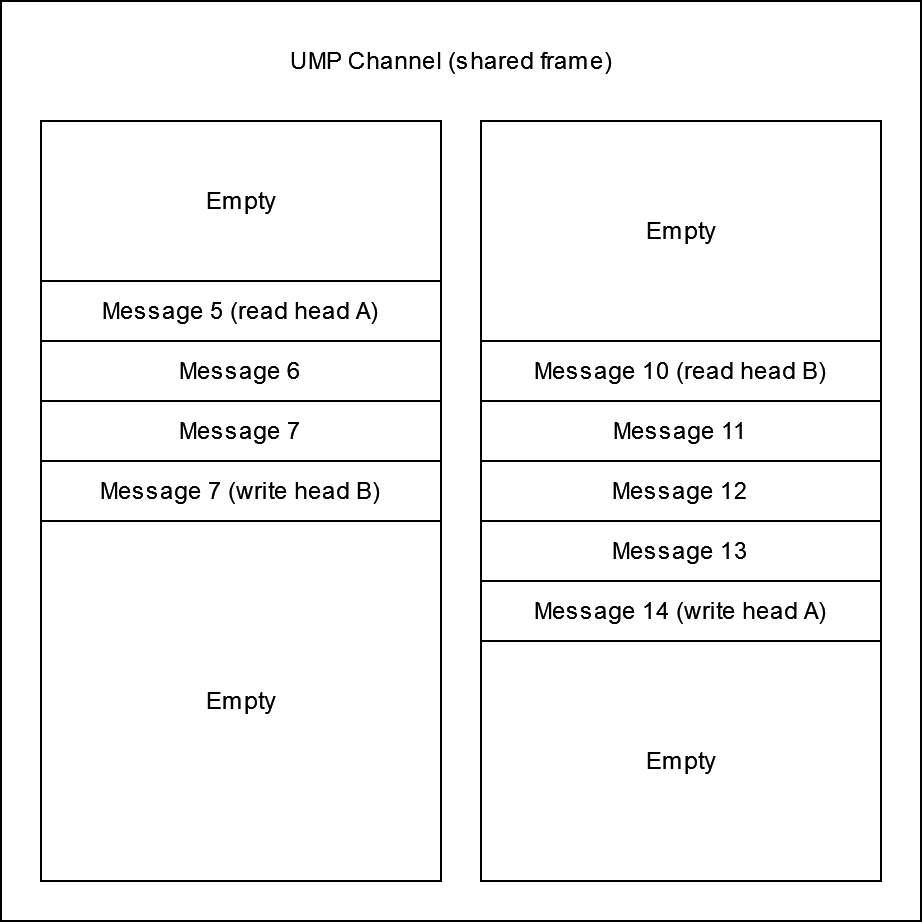
\includegraphics[width=12cm]{images/rpc/ump_chan.png}
    \caption{General structure of a UMP communication channel}
    \label{fig:rpc:umpchan}
\end{figure}

The contents of a single ump message are illustrated in figure \ref{fig:rpc:umpline}. Each message is as large as a single cache line. The first 56 bytes of the message hold the data to be sent, while the last 8 bytes are a control word holding the size of the message data in bytes\footnote{in retrospect, the control word only needs to be a single byte, not eight, as many of the size bits are wasted}, as well as a bit indicating whether the message of the higher-level protocol (discussed in the next section) was fragmented and more data follows in the next message.

\begin{figure}[htp]
    \centering
    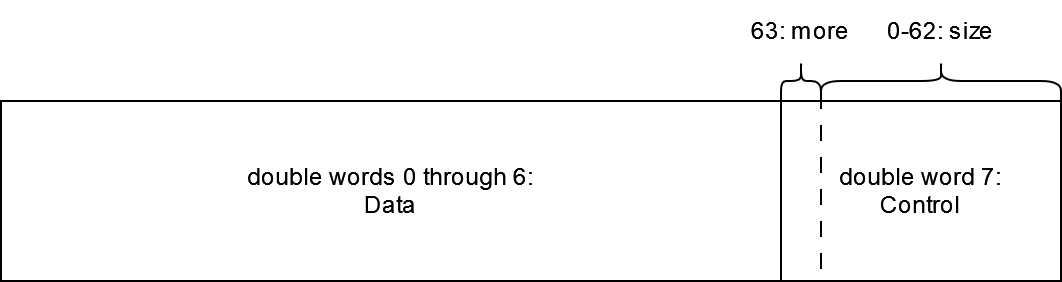
\includegraphics[width=12cm]{images/rpc/ump_line.png}
    \caption{The contents of a single cache line holding a UMP message}
    \label{fig:rpc:umpline}
\end{figure}

Listing \ref{listing:umpsend} shows the process of sending a UMP message on a channel. The ump channel object keeps track of the offset at which the next message should be sent. From there, the process consists simply of copying the data to be sent into the specified slot, followed by updating the control word. Importantly, a barrier is necessary between writing the data and setting the control word, to ensure that the receiver observes the update to the data before it starts reading it. There is no need for a barrier between checking if there is space in the channel and writing to it, as writes are never speculated\footnote{TODO reference to ARM manual}.

\begin{lstlisting}[caption={Sending a UMP message},label={listing:umpsend}]
static inline errval_t ump_chan_send(struct ump_chan* chan, const struct ump_msg* msg) {
    if (!ump_chan_can_send(chan)) {
        return LIB_ERR_UMP_CHAN_FULL;
    }
    
    // writes are never speculated, hence no barrier is necessary
    
    struct ump_line* line = chan->send.buf + chan->send.offset;
    memcpy(line->words, msg->data, msg->size);

    uintptr_t control = msg->size | (msg->more ? UMP_MSG_MORE : 0);

    // written data must be visible before control word
    dmb();

    line->words[UMP_CONTROL_WORD_IDX] = control;

    chan->send.offset = (chan->send.offset + 1) % chan->send.size;

    return SYS_ERR_OK;
}
\end{lstlisting}

The process of receiving a message is analogous, and shown in listing \ref{listing:umprecv}. We first check if the channel can receive a message, and, if it can, read out the data. We then set the control word to 0 to indicate to the writer that the slot is now clear.

In this case, two barriers are required: The first (on line 12) ensures that the data is not speculatively prefetched before the line is set to be valid by the sender, while the second (on line 17) ensures that the data is fully read before the sender can start writing to it again.
The control data can be read before the barrier because it is a direct data dependency of the condition.

\begin{lstlisting}[caption={Receiving a UMP message},label={listing:umprecv}]
static inline errval_t ump_chan_recv(struct ump_chan* chan, struct ump_msg* msg) {
    if (!ump_chan_can_recv(chan)) {
        return LIB_ERR_UMP_CHAN_EMPTY;
    }

    struct ump_line* line = chan->recv.buf + chan->recv.offset;
    uintptr_t control = line->words[UMP_CONTROL_WORD_IDX];
    msg->size = control & UMP_MSG_SIZE_MASK;
    msg->more = control & UMP_MSG_MORE;

    // avoid data being prefetched speculatively
    dmb();

    memcpy(msg->data, line->words, msg->size);

    // data must be read before clearing control word visible to writer
    dmb();

    // clear control word after reading data
    line->words[UMP_CONTROL_WORD_IDX] = 0;

    chan->recv.offset = (chan->recv.offset + 1) % chan->recv.size;

    return SYS_ERR_OK;
}
\end{lstlisting}

Finally, listing \ref{listing:umpcheck} shows how a message is defined to be (in)valid: If the control word is zero, the slot is empty and can be overwritten. On the other hand, if the control word is nonzero, it contains a message which can be read out. Note that this means that messages of length 0 are not supported, as that would imply the control word to be  zero for a valid message.
\begin{lstlisting}[caption={Checking if an entry is (in)valid},label={listing:umpcheck}]
static inline bool ump_chan_can_send(struct ump_chan* chan) {
    struct ump_line* line = chan->send.buf + chan->send.offset;
    return line->words[UMP_CONTROL_WORD_IDX] == 0;
}

static inline bool ump_chan_can_recv(struct ump_chan* chan) {
    struct ump_line* line = chan->recv.buf + chan->recv.offset;
    return line->words[UMP_CONTROL_WORD_IDX] != 0;
}
\end{lstlisting}

\section{Transport Layer}
To mitigate the additional complexity that arises when having to manage several different protocols at a time, as well as to avoid having to manage message fragmentation and metadata when implementing remote procedure calls and their respective handlers, LMP and UMP are abstracted under a common interface with message semantics. This interface is designed to allow for both blocking and non-blocking communication, to fragment and reassemble both the data and the capabilities being sent, as well as to almost completely abstract away the difference between LMP and UMP.

Once an rpc structure has been initialized using one of the LMP- or UMP-specific methods, there are several functions which can be used to interact with it to engage in communication.
The most important of these are 
\begin{enumerate}
    \item \texttt{aos\_rpc\_send\_with\_handler} and
    \item \texttt{aos\_rpc\_recv\_with\_handler}
\end{enumerate}
Both of these functions take as arguments a pointer to the rpc structure on which they are being invoked, as well as a a closure which is to be called once the respective operation finishes. \texttt{struct aos\_rpc} has members which describe the data to be sent, or the buffer to use when receiving data. These must be set before calling any functions for sending or receiving data.

Even though they are the most important interface for sending and receiving data through rpc, the above functions don't actually do much work themselves. Instead, they simply remember the corresponding handler closure in \texttt{struct aos\_rpc}, and then register an event handler for the underlying channel. Listing \ref{listing:sendhandler} shows the handler for sending messages. When the send handler is called, it tries to send a fragment of the message by using \texttt{transport\_try\_send}. This also updates internal offset values in \texttt{struct aos\_rpc}. Then, if more parts of the message remain to be sent, the handler is re-registered and, because the internal state was updated, on the next invocation, it will send the next part of the message. If no more parts of the message remain, the sending state is reset, and the handler which was originally set in \texttt{aos\_rpc\_send\_with\_handler} is invoked.

The interface for receiving data is completely analogous.

\begin{lstlisting}[caption={Send handler registered on waitset},label={listing:sendhandler}]
static void transport_send_handler(void *arg)
{
    errval_t        err = SYS_ERR_OK;
    struct aos_rpc *rpc = arg;

    bool more = false;
    err       = transport_try_send(rpc, &more);

    if (err_is_fail(err) 
        && !(lmp_err_is_transient(err) 
        || ump_err_is_transient(err))) {
        USER_PANIC_ERR(err, "transport_try_send");
    }

    if (more) {
        transport_register_send(
            rpc, MKCLOSURE(transport_send_handler, arg));
    } else {
        // reset send state
        rpc->send_offset      = 0;
        rpc->send_caps_offset = 0;
        if (rpc->send_handler.handler) {
            rpc->send_handler.handler(rpc, rpc->send_handler.data);
        }
    }
}
\end{lstlisting}

Listing \ref{listing:sendblocking} shows how \texttt{aos\_rpc\_send\_with\_handler} can be used to implement a blocking send operation, such as the one used for RPC calls, discussed in section \ref{section:rpc:rpc}. It consists of three main components:
\begin{enumerate}
    \item The data and capabilities which will be sent is set up in the rpc structure.
    \item A send operation is issued on the rpc structure, with a handler that updates a flag once the operation finishes.
    \item Events are dispatched on the waitset associated with the rpc structure until the closure signals that the send operation has concluded.
\end{enumerate}

\begin{lstlisting}[caption={Using \texttt{aos\_rpc\_send\_with\_handler} for a blocking send implementation},label={listing:sendblocking}]
static void _blocking_closure(struct aos_rpc *rpc, void *data)
{
    (void)rpc;
    *(bool *)data = false;
}

errval_t aos_rpc_send_blocking_varsize(struct aos_rpc *rpc, const void *buf, size_t size,
                                       struct capref *capbuf, size_t capsize)
{
    errval_t err = SYS_ERR_OK;

    err = _lmp_init_late_client(rpc);
    if (err_is_fail(err)) {
        return err;
    }

    // set the data to be sent
    rpc->send_buf.data = (void *)buf;
    rpc->send_size     = size;
    rpc->send_buf.size = size;

    // set capabilities to be sent
    rpc->send_buf.caps  = capbuf;
    rpc->send_caps_size = capsize;

    bool waiting = true;
    aos_rpc_send_with_handler(
        rpc, MKHANDLER(_blocking_closure, &waiting));
    // block until the send operation has been finished
    while (waiting) {
        err = event_dispatch(rpc->waitset);
        if (err_is_fail(err)) {
            return err;
        }
    }

    return err;
}
\end{lstlisting}

\section{A detour: The init process and blocking operations}
\label{section:rpc:initnoblock}
In our design, each core's respective init process is the coordinator through which almost all operations are performed, from memory allocation to process management or file system operations. They are either performed in-process (by using the RAM allocator within the init process, for example) or forwarded to another process for handling, for example for performing operations on  the file system.

Because most of init's work consists of communication (either with user processes or the other init process), we decided on a fully asynchronous and non-blocking design. There is only a single thread which is dispatching events on the default waitset. When an operation needs to wait until a later point in time, a callback is registered and other operations are executed in the meantime.

This design has several advantages, the most obvious being that we are able to completely avoid any synchronization through mutexes, condition variables, etc. Basically, all perils of multi-threaded programming are avoided. Furthermore, we also avoid the need for keeping around waiting threads to handle events for user processes. It may be reasonable to say that this is the leanest-possible design for a centralized init process. This, however, means that it is of paramount importance to ensure that \textit{no} blocking operations are used in init

There are, however, also issues with our approach: Asynchronous programming is difficult when the programming language provides absolutely no language features to facilitate it. Especially for operations which may need to suspend multiple times, keeping around local variables in special \texttt{struct}s is tedious and error-prone, and manually registering callbacks quickly obscures the actual flow of control.

\section{Remote Procedure Calls}
\label{section:rpc:rpc}
Between user processes and the respective init processes on the same core, we employ an interface structured around blocking remote procedure calls. Importantly, these calls are \textit{only} blocking to the user processes. The init process, as stated previously, never blocks.

When a process is spawned, a communication channel is automatically set up between the spawned process and the init process executing the spawn. In fact, the structure keeping track of the communication state between init and the spawned process is part of the \texttt{struct spawninfo} which keeps track of various kinds of state related to the process. The fact that there is only a single \textit{blocking} communication channel between each process and init naturally implies that all RPCs originating from a single process are serialized, and cannot occur concurrently. We will discuss this in more detail when talking about the limitations of our system in section \ref{section:rpc:limitations}.

Because all RPCs are issued through a single communication channel, a common protocol is required such that the init process knows which handler to call when a request arrives.
We achieve this by using a hierarchy of structs, with an enumerator containing all possible request types at the base level. Listing \ref{listing:rpcstruct} shows an excerpt of this hierarchy. It also highlights how flexible array members can be used for sending arbitrarily large messages (useful for sending strings, for example) across the rpc channel.

\begin{lstlisting}[caption={A hierarchy of request types},label={listing:rpcstruct}]
struct aos_generic_rpc_request {
    enum {
        AOS_RPC_REQUEST_TYPE_MEMSERVER,
        AOS_RPC_REQUEST_TYPE_TERMINAL,
        /* ... */
        AOS_RPC_REQUEST_TYPE_PROC_MGMT,
    } type;
};

struct aos_proc_mgmt_rpc_request {
    struct aos_generic_rpc_request base;
    enum {
        AOS_RPC_PROC_MGMT_REQUEST_SPAWN_CMDLINE,
        AOS_RPC_PROC_MGMT_REQUEST_STATUS,
        /* ... */
        AOS_RPC_PROC_MGMT_REQUEST_NAME,
    } proc_type;
    coreid_t core;
};

struct aos_proc_mgmt_rpc_spawn_request {
    struct aos_proc_mgmt_rpc_request base;
    char cmdline[];
};
\end{lstlisting}

\subsection{Performing the Call}
From the perspective of a user process, an rpc call consists of the following steps:
\begin{enumerate}
    \item Marshal the arguments into the appropriate structure
    \item Send the structure (and capabilities, if any need to be sent) into the channel using the blocking send operation.
    \item Receive the response from init using a similar blocking receive operation.
    \item Unmarshal the return values and return them to the original caller.
\end{enumerate}
During steps 2 and 3, the user thread making the request becomes blocked. While other user threads may still make progress during this time, no rpcs can be issued concurrently.

\subsection{Handling the Call}
Because init must never block, it cannot use blocking receive operations to wait for RPC requests from a user process to arrive. Instead, it uses \texttt{aos\_rpc\_recv\_with\_handler} to defer until a message actually arrives from the process. Even though there may be many processes, each with their own rpc endpoint, because all are registered on the same waitset which is being continuously dispatched on, init is able to handle requests from all user processes concurrently.

At the core of the rpc system lies the handler closure registered using the previously mentioned receive call. It receives as arguments the message that was received, as well as a handle to the rpc endpoint to which the reply should be sent. When handling rpc requests, there are generally two cases of differing complexity.

In the simplest case, the request can be processed and a reply can be sent \textit{immediately}, without any sort of waiting operation required. In this case, a reply can be sent using \texttt{aos\_rpc\_send\_with\_handler} directly from the handler function. This is the case for many simpler rpc requests, for example memserver requests on core 0.

Things get more complicated when the reply cannot be sent immediately, such as when waiting for a process to terminate. Because init is non-blocking, the handler function cannot simply wait until the target process terminates: This would block the system until that point, and would probably cause a deadlock if the waited-for process also tried to make an rpc. Instead, a callback is registered registered within the process management system to be called when the target process terminates. This callback will then send the actual reply to the original caller. Because the stack frame of the handler will already be long gone, it is important to preserve necessary information accross this suspension point.

For handling requests concerning distributed capabilities, up to three suspensions may be required to handle a single call (wait until capability is unlocked, wait until revoke finishes on other core, wait until revoke finishes on own core). Due to the lack of asynchronous programming support in C, this process quickly becomes tedious.

\section{Asynchronous Message Passing}
\label{section:rpc:async}
Some user requests require communication between the init processes on the two cores. Because only a single communication channel is available, and the init processes must be non-blocking, a different communication system was required for cross-core synchronization. The main requirement for this system is that requests can "overtake" each other: A short request which can be executed and responded to immediately should not block when waiting for a long-running request such as a \texttt{wait} operation. This is best explained in an example:

Imagine two processes, \texttt{p0.0} and \texttt{p0.1}, both on core 0. Now, \texttt{p0.0} makes a \texttt{wait} rpc request for a process on another core. The request will first be sent to init on core 0, which will forward it to core 1, where a callback will be registered in the process management system. Now, \texttt{p0.1} performs a \texttt{cap\_delete} operation which needs to synchronize across cores. 
We desire our cross-core rpc system to be flexible enough to allow
\begin{itemize}
    \item the synchronization request to be made before the wait request has returned.
    \item a reply to the synchronization request to be sent before the wait request has been replied to.
    \item core 1 to issue requests concurrently to handling requests coming from core 0.
\end{itemize}
Neither of these requirements are satisfied by the rpc system described previously.

For this purpose, we devised the \texttt{async\_channel}. It has a very simple interface, consisting of the two functions shown in listing \ref{listing:asyncinterface}.

\begin{lstlisting}[caption={The interface for \texttt{async\_channel}},label={listing:asyncinterface}]
void async_init(struct async_channel *async, struct aos_rpc *rpc,
                async_request_handler handler);
void async_request(struct async_channel *async, void *data, 
                   size_t size, struct capref *capv,
                   size_t capc, async_callback callback, 
                   void *meta);
void async_respond(struct async_channel *async, 
                   struct response *res);
\end{lstlisting}

An \texttt{async\_channel} is initialized on top of a standard \texttt{aos\_rpc} instance. In our implementation, this is always the cross-core channel communicating through UMP. Similarly to the standard rpc server interface, a handler function is also passed upon initialization. This function is called with the request parameters whenever a request arrives, and should schedule \texttt{async\_respond} to be called at some point in the future. Once the response arrives, the \texttt{async\_callback} provided in the initial request is called.

\subsection{Design Details}
Because there is only one cross-core channel, but requests and responses may originate from either core, we multiplex requests and responses on a single communication channel. Furthermore, we allow responses to later requests to be sent before responses to earlier requests. 

This is visually illustrated in figure \ref{fig:rpc:asyncchan}: Core 0 is sending requests with id 13 and 14, while a response to a request issued by the other core is interspersed in the middle. On the other hand, core 1 is replying to requests 2 and 9 out of order, on the same channel used for sending request 12.

\begin{figure}[htp]
    \centering
    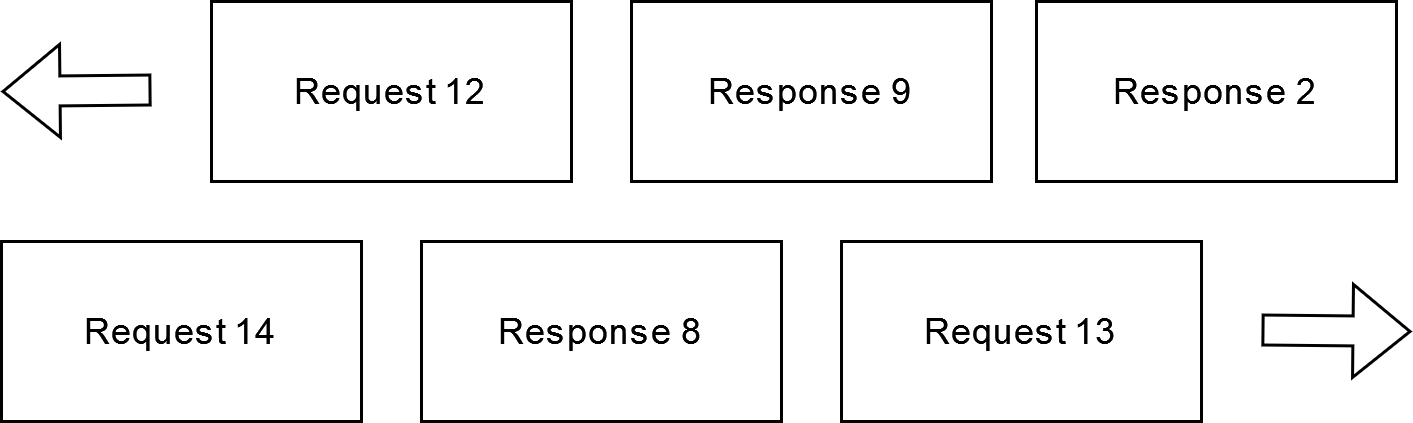
\includegraphics[width=12cm]{images/rpc/async_channel.png}
    \caption{Multiplexed and out-of-order requests and responses}
    \label{fig:rpc:asyncchan}
\end{figure}

\subsection{An Example Request}
\label{subsec:rpc:examplereq}
Let us now consider the life cycle of an example request.
\begin{enumerate}
    \item The request is issued using \texttt{async\_request}. The function allocates a request queue node and appends it to the queue of pending requests of the channel. 
    \item Once it is at the head of the queue, the request is dequeued and sent across the underlying communication channel. Importantly, the request node is \textit{not deallocated}.
    \item The request arrives on the other core, a response object is allocated, and the handler function is called with the data and the response object.
    \item At some point in the future, \texttt{async\_respond} is called on the response object. It is appended to the response queue of the channel.
    \item Once the response is at the head of the queue, it is sent across the channel and the object is deallocated.
    \item The response arrives on the other core, and the handler function provided during the initial request is called.
    \item The original request object is deallocated.
\end{enumerate}

Most steps of this process are straightforward: Sending and receiving messages simply uses \texttt{aos\_rpc\_send\_with\_handler} and \texttt{aos\_rpc\_recv\_with\_handler}, where the respective handler functions simply dequeue more messages or call the handler function registered on the channel. However, there is one significant design question remaining: When a response arrives, how do we find the callback provided during the initial request?

A possible solution would be to use a hash map and associate each request with an identifier. Then, the response simply needs to carry the same identifier as the request, and the data for the correct request can be retrieved. However, because both ends of the communication channel are trusted, we can actually use a much simpler and efficient solution, as shown in listing \ref{listing:asyncmessage}: We simply pass along the address of the request structure allocated in the first step of the \texttt{async\_request}, as explained in \ref{subsec:rpc:examplereq}. This same address is also returned in the response. Then, once a response arrives, we can directly call the handler. The entire process is shown in listing \ref{listing:asyncrecvhandler}.

\begin{lstlisting}[caption={The message type used on the async channel},label={listing:asyncmessage}]
struct async_message {
    struct request     *identifier;
    enum async_msg_type type; // ASYNC_RESPONSE or ASYNC_REQUEST
    size_t              size;
    size_t              capc;
    char                data[];
};
\end{lstlisting}

\begin{lstlisting}[caption={Propagating and directly accessing message identifiers},label={listing:asyncrecvhandler}]
if (msg->type == ASYNC_RESPONSE) {
    // get original request object corresponding to response
    struct request *req = msg->identifier;
    // call callback
    req->callback(req, data, msg->size, capv, msg->capc);
    // free request object
    free(req);
} else if (msg->type == ASYNC_REQUEST) {
    // allocate response
    struct response *res = malloc(sizeof(struct response));
    res->identifier      = msg->identifier;
    res->finalizer       = free_finalizer;
    res->next            = NULL;
    // call handler and give it ref to response
    async->response_handler(
        async, data, msg->size, capv, msg->capc, res);
} else {
    USER_PANIC("Invalid async message type");
}
\end{lstlisting}

\subsection{Sending Capabilities}
Because \texttt{async\_channel} is the only communication channel between the init processes on the two cores, we also use it to implement cross-core capability transfers, as enabled by the distributed capability system (discussed in chapter \ref{chapter:distcap}). This allows requests to be transparently relayed to the other core.
This functionality is enabled by using \texttt{cap\_transfer\_move} when a message is queued for sending and \texttt{cap\_from\_transfer} when it is received on the other core. A more detailed discussion can be found in chapter \ref{chapter:distcap}.

\section{Retrospective}
\label{section:rpc:limitations}
In our design, the most impactful decision was probably to make init single-threaded, asynchronous and fully non-blocking. In a programming language with strong support for asynchronous operations, such as Rust or Zig, this design would probably be the clear winner: It completely avoids all issues related to thread-level parallelism, eliminates the need for synchronization, and is highly memory-efficient when compared to threads. However, in retrospect, it is not clear whether such a design is the best decision, especially when factoring in the significant cognitive overheads of programming asynchronously in C. We may have been able to achieve a similarly performant implementation by spawning an rpc handler thread in the init process for every user process. 
This, however, would not address the most significant limitation of our system: Only a single rpc can be performed concurrently from each user process. A solution to this would be to leverage the same async channel implementation that we used for cross-core communication for handling communication between user processes and init. While this would introduce additional overheads from dynamic allocations, it would make the system more flexible and capable.

% \input{urpc.tex}
\chapter[Multi-core Support]{Multi-core Support \\ \Large \textnormal{Group Milestone}}


\section{Introduction}

\href{https://en.wikipedia.org/wiki/Multi-core_processor}{\texttt{Multicore processors}} are computer chips that have multiple independent \texttt{processing units}, called \texttt{cores}, on a single chip. Each core functions like a \texttt{separate processor}, capable of executing instructions and performing tasks. With multiple cores, a multicore processor can handle multiple tasks simultaneously, improving overall performance and efficiency. It's like having multiple workers in a team, each working on different tasks at the same time, making the work faster and more efficient. Multicore processors are standard in computer systems today.

Our current operating system has the capability to run multiple programs, but it's limited to running them on a \texttt{single core}. To enhance its functionality and allow it to run programs \texttt{simultaneously} on \texttt{multiple cores}, we need to enable multicore processing. This involves \texttt{booting} a second core in the system.

Once the second core is successfully booted, we face the challenge of managing the available physical memory between the two cores. Both cores need to have access to memory resources while avoiding conflicts or overlaps. Additionally, we need to establish a means of communication between the two cores to facilitate \texttt{coordination} and \texttt{data exchange}.

\subsection{Steps required to boot the second code}

\texttt{Barrelfish} is a \texttt{microkernel}. This implies that most of the work need to be done in \texttt{user space} to prepare the new CPU driver for booting. We need to allocate memory for various components and provide necessary information. This represents an overview of the essential steps.

\begin{itemize}
\item \textbf{Allocate Memory}: The new \texttt{CPU} driver requires memory for loading the boot driver, loading the CPU driver itself, a core data structure, a kernel stack, space for the init process, a URPC frame for cross-core communication channels, and a new KCB (kernel control block). We can allocate these as separate frames or in a contiguous block. To obtain a new KCB, we can retype a RAM cap into a KCB and initialize the \texttt{armv8\_core\_data structure}.

\item \textbf{Load and Relocate the Boot/CPU Driver}: Loading the \texttt{ELF} file for the CPU driver is similar to loading user-level processes. There are provided support functions, \texttt{load\_elf\_binary} and \texttt{relocate\_elf}, that handle \texttt{loading} and \texttt{relocation} and determine the \texttt{entry points} of the boot driver and the CPU driver. The boot driver's entry point for PSCI is called \texttt{boot\_entry\_psci}, and the physical address of this symbol is needed later. 

\item \textbf{Fill in the armv8\_core\_data Structure}: We need to fill the fields in the \texttt{armv8\_core\_data} structure.Provide information such as the initial task (\texttt{monitor\_binary}), memory for the initial task, location of the URPC frame, kernel command line, virtual CPU driver entry point (\texttt{cpu\_driver\_entry}), stack for the CPU driver (\texttt{cpu\_driver\_stack}), and the correct \texttt{boot magic} (PSCI).

\item \textbf{Clean the cache}: It is essential to ensure that the initialized data is visible to an uncached observer, which means that we need to perform \texttt{cache flushing}.

During the cache cleaning process, any data that has been modified or written to the cache is synchronized and written back to the main memory. This ensures that the latest data is available and visible outside the cache, making it accessible to other components or observers that do not utilize the cache.

By performing cache flushing, we guarantee \texttt{data coherence} and \texttt{consistency} between the cache and the main memory.

\item \textbf{Invoke the Kernel Cap}: The last step involves invoking a specific operation on the kernel capability, utilizing a boot protocol defined by the hardware platform. In our case, we are using the \texttt{armv8 architecture}. This operation is responsible for initiating the boot driver, and consequently, the CPU driver, on the designated core.
\end{itemize}

The exact details of this boot algorithm depend on the specific \texttt{hardware architecture} being used. It outlines the necessary instructions and procedures to effectively start the boot driver, enabling the subsequent execution of the CPU driver on the targeted core.

By invoking this operation, we trigger the necessary mechanisms for the boot process, ensuring that the boot driver and CPU driver are properly initiated.

These steps are part of the process of booting a second core in an operating system using Coreboot.

\section{Booting the second core - our implementation}

Within this section, we will outline the sequential steps involved in the process of booting a second core. These steps provide a systematic approach to successfully initiate and integrate the additional core into the system's operation.

To ensure clarity and facilitate understanding, each step will be thoroughly explained, ensuring that you have a complete understanding of the process from start to finish. By following these steps in the specified order, you can effectively enable the utilization of the second core, expanding the system's computational capabilities.

Through this sequential breakdown, we aim to provide a clear overview of the tasks and considerations involved in booting a second core. 

\subsection{Creation of the KCB}

The process of creating the \texttt{Kernel Control Block} (KCB) operates as follows. First, we initiate a request for a specific amount of RAM (random-access memory) from the system. Ideally, this request should result in the allocation of a capability, granting access to the memory area. The size of this capability should match the predetermined size of \texttt{OBJSIZE\_KCB}, and it should adhere to the alignment requirements specified by \texttt{KCB\_ALIGNMENT}.

With the allocated slot in place, we can proceed to retype the obtained \texttt{capability} into the corresponding type, which in this case is \texttt{ObjType\_KernelControlBlock}. This step involves transforming the general capability into a specific type that represents the \texttt{KCB}. By performing this retype operation, we establish a clear association between the allocated capability and its purpose as a \texttt{KCB}.

The creation of the \texttt{KCB} involves requesting and obtaining a specific memory capability, allocating a slot for it, and subsequently retype it to the appropriate \texttt{ObjType\_KernelControlBlock} type. These steps ensure that the \texttt{KCB} is properly set up and ready to serve as the central structure holding the state and information necessary for a kernel instance within the operating system.

\subsection{Load the bootloader, cpu driver}

The process of loading the \texttt{bootloader} and the \texttt{cpu driver} required the execution of a series of steps in a methodical manner. Let's delve into these steps and their respective functions.

Firstly, we initiate the process by locating the module using the \\texttt{load\_module\_into\_memory} function, which requires specifying the path to the desired module. This function enables us to identify and retrieve the module necessary for further processing.

Once we have successfully located the module, the next step involves mapping it into the \texttt{virtual address space}. This mapping operation allows us to establish a connection between the module and the virtual memory layout of the system. By mapping the module into virtual space, we can gain direct access to its contents and perform subsequent operations on it.

Having mapped the module in the virtual address space, we proceed to copy its contents into another frame. This involves duplicating the module's data and storing it in a separate frame of memory. This new frame, housing the copied module data, is also mapped into the \texttt{virtual address space}. Through this process, we acquire a capability that encapsulates the corresponding module.

With the capability in hand, we can retrieve the entry point of the module. The entry point serves as the designated starting point for execution within the module's code. Subsequently, we load the \texttt{ELF binary} associated with the module, incorporating it into the system's memory.

Finally, we proceed with the \texttt{relocation} of the \texttt{ELF binary}. Relocation involves adjusting memory addresses and \texttt{resolving symbol references} within the binary to align with the virtual memory layout. 

\subsection{Load the monitor process}

The process of loading a program bears significant resemblance to that of loading the \texttt{boot loader} and the \texttt{CPU driver}. However, there is a notable difference in that we are exclusively concerned with loading a binary image in the ELF format. As a result, we do not need to perform the \texttt{relocation} of the ELF at this particular stage of the process. Instead, the relocation step will be carried out later by the CPU driver.

In this context, loading the program involves retrieving the binary image in ELF format and preparing it for execution. Unlike the boot loader and CPU driver, which require relocation to align memory addresses and resolve symbol references, the program being loaded does not undergo this relocation process immediately. This will be done in the cpu driver.

\subsection{Allocate the core data structure and stack}

At this stage of the process, we have gathered all the necessary components and resources required to populate the core data structure comprehensively. This allows us to provide crucial information and configurations for the proper functioning of the second core. Below is a list outlining the steps required to populate the core data structure.

\begin{itemize}
    \item Include the capability used for the CPU stack frame within the core data structure. This capability enables the second core to have access to the designated stack space for executing tasks and managing its own stack operations effectively.

    \item Pass the command line arguments specifically intended for the \texttt{app\_main} function, which serves as the \texttt{entry point} in the C code for the second core. These arguments can provide essential parameters or instructions that are required for the proper execution of the core's tasks and functions.

    \item Load the CPU memory frame, which encompasses the memory region specifically allocated for the second core's usage. By providing this information within the core data structure, we ensure that the core can efficiently manage and utilize its allocated memory resources.

    \item Fill the monitor binary details within the core data structure. The monitor binary serves as an integral component in the system, responsible for overseeing the functioning of the core and facilitating coordination between different cores within the system.

    \item Specify the base address of the \texttt{Kernel Control Block} block within the core data structure. The \texttt{KCB} block acts as a fundamental structure holding critical state and information for the kernel instance running on the second core.

    \item Finally, minor but important operations are performed to ensure the completeness and accuracy of the core data structure. These operations may involve configuring various parameters or fields within the structure to ensure optimal integration of the second core into the system.
    
\end{itemize}

\subsection{Flush the cache}

Prior to writing any data to the second core, it is essential to perform a \texttt{cache flush} operation to ensure that the content of the core data structure is accurately visible to the other core. This cache flush procedure guarantees that any modifications or updates made to the core data structure are synchronized and reflected in the cache, making them accessible to other cores or components that rely on the cache for data retrieval.

To accomplish this cache flushing process, we make use of two specific functions: \texttt{arm64\_dcache\_wb\_range} and \texttt{arm64\_idcache\_wbinv\_range}. These functions serve distinct purposes in the cache maintenance process.

The \texttt{arm64\_dcache\_wb\_range} function is responsible for synchronizing the modified or written data in the data cache with the main memory, ensuring that the latest version of the data is stored in the memory. This ensures that any subsequent read operations from other cores or system components fetch the most up-to-date information.

On the other hand, the \texttt{arm64\_idcache\_wbinv\_range} function is involved in the \texttt{invalidation} and \texttt{write-back} operations for the instruction cache. It ensures that any modifications made to the instruction cache are written back to the main memory and the cache is invalidated, ensuring that subsequent instruction fetches reflect the latest changes made to the core data structure.

By invoking these cache maintenance functions, we guarantee cache coherence and ensure that the second core can accurately perceive and access the current state of the core data structure. This \texttt{synchronization} is crucial for booting the second core.

\subsection{invoke\_monitor\_spawn\_core}

Now, we reach the final stage of the process for booting a second core. At this point, we have successfully created all the necessary memory allocations required for the booting process. Additionally, \texttt{the armv8\_core\_data} structure has been filled with the accurate and appropriate values.

With the allocated memory in place and the \texttt{armv8\_core\_data} structure properly configured, we have effectively laid the foundation for the successful booting of the second core. These preparations ensure that the core has access to the essential resources it needs to begin executing tasks and contributing to the overall operation of the system.

At this stage, we are ready to execute the function \texttt{invoke\_monitor\_spawn\_core}, which plays a crucial role in the process of waking up the second core of the computer through a system call.

By making this function call, we signal the operating system and the underlying firmware to take the necessary steps to awake the second core, allowing it to join the primary core in executing tasks and contributing to the overall computational capabilities of the system.

\begin{lstlisting}[caption={Output of the first core},captionpos=b,frame=single,breaklines]
kernel 1: ARMv8-A: Global data at 0xffff000040000000
kernel 1: ARMv8-A: Kernel stack at 0xffff0000bc0ad000.. 0xffff0000bc0bd000
kernel 1: ARMv8-A: Kernel first byte at 0xffff0000bc05e000
kernel 1: ARMv8-A: Exception vectors (VBAR_EL1): 0xffff0000bc05e800
kernel 1: GICv3: Enabling CPU interface
kernel 1: GICv3: CPU interface enabled
kernel 1: ARMv8-A: Enabling timers
System counter frequency is 62500000Hz.
Timeslice interrupt every 5000000 ticks (80ms).
kernel 1: ARMv8-A: Setting coreboot spawn handler
kernel 1: ARMv8-A: Calling arm_kernel_startup
kernel 1: ARMv8-A: Doing non-BSP related bootup 
kernel 1: ARMv8-A: Memory: bc0c2000, bc696000, size=5968 kB
kernel 1: ARMv8-A: spawning 'armv8/sbin/init' on APP core
kernel 1: ARMv8-A: spawn_init_common armv8/sbin/init
spawn module: armv8/sbin/init
kernel 1: init page tables: l0=0xffff0000bc3a0000, l1=0xffff0000bc3a1000, l2=0xffff0000bc3a2000, l3=0xffff0000bc3a3000
kernel 1: ARMv8-A: creating monitor URPC frame cap
\end{lstlisting}

\subsection{Bootinfo setup}

The last step for the second core to be operational is to copy the bootinfo, containing information on the different module available and capabilities of the hardware to the new core. The bootinfo includes two part: the memory region descriptions which can be sent by RPC to the new core and the memory capabilities. 

Because (without considering the capabilities revisited milestone), it is not possible to send capabilities to another core, these needs to be forged, which is a process to create new capabilities (and as such is unsafe). This process is only used to create the bootinfo capabilities in the second core. These capabilities come as RAM, physical addresses or frames, and their capabilities have specific predetermined location to be in. We use the following code to handle all these cases:

\begin{lstlisting}[caption={Forging bootinfo capabilities},captionpos=b,frame=single,breaklines]
for(size_t i = 0; i < bi->regions_length; i++){
    errval_t (*forge_function)(struct capref, genpaddr_t, gensize_t, coreid_t) = NULL;
    struct capref* cap = NULL;
    gensize_t map_size = bi->regions[i].mr_bytes;

    switch (bi->regions[i].mr_type)
    {
    case RegionType_Empty:
        forge_function = ram_forge;
        cap = &mem_cap;
        break;

    case RegionType_PhyAddr:
    case RegionType_PlatformData:
        forge_function = physaddr_forge;
        cap = &phys_cap;
        break;

    case RegionType_RootTask:
        forge_function = frame_forge;
        cap = &frame_cap;
        break;

    default:
        break;
    }

    if(forge_function != NULL && cap != NULL){
        map_size = ROUND_PAGE_UP(map_size);
        err = forge_function(*cap, bi->regions[i].mr_base, map_size, disp_get_core_id());
        if(err_is_fail(err))
            return err;
        cap->slot++;
    }
}
\end{lstlisting}

\section{Technical comments}

\subsection{Difference between the \texttt{boot driver} and the \texttt{cpu driver}}

The boot driver plays a crucial role in the system as the \texttt{final-stage bootloader} responsible for initializing the Memory \texttt{Management Unit (MMU)} for the CPU driver. It serves as a critical component that sets up the essential environment and conditions before \texttt{transferring control} to the CPU driver.

In essence, the boot driver takes on the responsibility of configuring the system and establishing a stable and known state for the subsequent execution of the CPU driver. It performs various initialization tasks, such as setting up memory mappings, configuring hardware registers, and preparing the necessary data structures required for the CPU driver's operation.

One of the primary functions of the boot driver is to ensure the proper setup of the MMU. The MMU is a hardware component responsible for virtual memory management, providing address translation and memory protection features. By configuring the MMU, the boot driver puts the \texttt{virtual address space} in a \texttt{known state}.

Once all the critical data structures are established, and the overall system is in a \texttt{known and stable state}, the boot driver hands over control to the CPU driver. At this point, the CPU driver takes the lead and continues with the remaining tasks and operations required for the system's functionality.

The transition from the boot driver to the CPU driver signifies a significant turning point in the system's execution. The CPU driver assumes responsibility for managing the core's execution, coordinating tasks, and executing the desired operations based on the established environment and data structures set up by the boot driver.

In summary, the boot driver acts as the \texttt{final-stage bootloader}, responsible for configuring the MMU, setting up the system environment in a known state, and transferring control to the CPU driver. It ensures that all necessary data structures are prepared, and the system is in a known state before handing over control. The CPU driver then takes charge, carrying out the subsequent operations and tasks required for the system's overall functionality.

\subsection{bsp\_main vs app\_main}

\texttt{Barrelfish} employs a clear distinction between the \texttt{Bootstrap (BSP) processor} and the \texttt{Application (APP) processors}. This distinction becomes apparent during the boot process of the computing device.

The \texttt{BSP} processor, also known as the bootstrap processor, holds a unique position as the \textbf{first processor to be booted} when the board is powered on. It serves as the initial point of entry into the system and plays a critical role in initializing the system's core components and establishing the foundational environment.

In the C code of the \texttt{Barrelfish} operating system (at least in the given code for the course), the \texttt{bootstrap processor} follows a specific execution path defined by the \texttt{bsp\_main} function. This function contains the code that guides the \texttt{bootstrap processor} through the essential initialization steps, such as configuring hardware, setting up system resources, and establishing the fundamental framework required for subsequent operations.

On the other hand, the \texttt{APP processors} refer to the additional processors or cores present in the system, apart from the bootstrap processor. When these \texttt{APP processors} are booted, they take on the role of application processors, focusing on executing application-specific tasks and functionalities. They won't execute the file system or the shell for example.

In the C code structure, the \texttt{APP processors} follow a distinct execution path defined by the \texttt{app\_main} function. This function serves as the \texttt{entry point} for the \texttt{APP processors}, where the specific application-related operations and processes are executed.

\subsection{Physical memory and virtual memory}

Now, let's focus on the \texttt{memory model}, emphasizing the contrasting memory access modes utilized by the boot driver and the CPU driver. The boot driver plays a vital role in putting the system into a known state during the booting process. It operates exclusively in the realm of \texttt{physical addressing} since the MMU (Memory Management Unit) has not yet been set up. This implies that all operations must be conducted using \texttt{physical memory addresses}.

Within the core data structure, an essential piece of information is the physical address indicating the starting point of the bootloader. The bootloader assumes the responsibility of configuring a minimal set of paging data structures exclusively dedicated to the CPU driver. During the booting process, the boot driver sets up the necessary minimal paging structures and activates the MMU, enabling the CPU driver to work seamlessly with \texttt{virtual memory}. These data structures lay the foundation for efficient \texttt{virtual memory management}, enabling the CPU driver to interact with the system using \texttt{virtual memory addresses}. It is important to note that the CPU driver exclusively operates within the \texttt{virtual memory domain}.

This distinction highlights a critical difference between the CPU driver and the block driver. While the \textbf{CPU driver relies on virtual memory} for its operations, \textbf{the block driver can directly access and manipulate physical addresses}. This disparity arises due to the differing requirements and functionalities of these components within the system. On has to set the virtual address space in a known state and the second actually needs.

\section{Retrospective}
We decided to work on user-level message passing and multi-core support concurrently, to be able to integrate proper cross-core communication from the start, instead of having to switch to a different solution later. This worked quite well: Having the full suite of \texttt{aos\_rpc} functions available for initializing the other core streamlined the process considerably, as it already provided support for message fragmentation, callbacks, etc.


\definecolor{shell_default}{HTML}{e4e4e4}
\definecolor{shell_background}{HTML}{272a36}
\definecolor{shell_command}{HTML}{59f68e}
\definecolor{shell_quote}{HTML}{f4f89d}
\definecolor{shell_variable}{HTML}{ff93d0}
\definecolor{shell_file}{HTML}{99ecfe}
\definecolor{shell_operator}{HTML}{c9a8fb}
\definecolor{shell_escape}{HTML}{99ecfd}

\lstset{
    literate={~} {$\sim$}{1}
}

\def\shellquote{\textcolor{shell_escape}{\texttt{\string\"}}}
\def\shellrawquote{\textcolor{shell_default}{\texttt{"}}}

\lstdefinestyle{ShellInputStyle}{
  language=bash,
  basicstyle=\small\sffamily\ttfamily,%
  numbersep=3pt,
  frame=tb,
  columns=fullflexible,
  backgroundcolor=\color{shell_background},
moredelim=**[is][\color{shell_variable}]{@}{@},
moredelim=**[is][\color{shell_operator}]{+}{+},
moredelim=**[is][\color{shell_file}]{§}{§},
moredelim=**[is][\color{shell_command}]{!}{!},
moredelim=**[is][\color{shell_quote}]{\%}{\%},
moredelim=**[is][\bfseries]{^}{^},
linewidth=0.95\linewidth,
  xleftmargin=0.1\linewidth,
  stringstyle=\color{shell_quote},
keywordstyle=\color{shell_command},
moredelim = [s][\color{purple}]{\\[}{\\]},
morekeywords={run, time, wc, tee},
basicstyle=\footnotesize\ttfamily\color{shell_default},
morestring=*[d]{"},
morestring=[s][]{\#\{}{\}},
escapeinside={\%*}{*}
}


\chapter[Shell]{Shell \\ \Large \textnormal{Jan Luca Scheerer}}
\label{chapter:shell}

The shell plays a crucial role in the functionality and versatility of any operating system. Acting as the bridge between the user and the underlying system, the shell provides a powerful interface for executing commands, managing processes, and manipulating files and directories. 

In this chapter, we delve into the milestones of enhancing the UART driver and implementing essential features of the shell. We begin by covering the extension of the UART driver, followed by a detailed discussion on the core functionality of the shell. This functionality includes syntax highlighting, tab completion, and the ability to define custom session variables.

To further explore the capabilities of the shell, we conclude this chapter by examining its advanced features. These features include support for executing lists of commands and command pipelines, enabling both I/O redirection and pipes.

\section{Userspace UART Driver}

As outlined in Chapter \ref{chapter:mp}, all RPC services are coordinated by each core's respective init process, and potentially forwarded to a different core's init process, if the request cannot be completed \emph{locally}. The userspace UART driver conforms to this paradigm: it runs as part of \texttt{init.0}, and any serial request addressed to a different core's init process will relay the request to \texttt{core 0}.

The driver is set up following the guidelines and instructions provided in the relevant section of the AOS Book. First, we initialize the GIC distributor driver by mapping the GIC to the current address space and calling \texttt{gic\_dist\_init}. Next, we initialize the \texttt{LPUART} driver by once again mapping the corresponding device frame into our address space and calling the appropriate initialization function - \texttt{lpuart\_init}. Having initialized both the GIC distributor and the \texttt{LPUART} drivers, we can now allocate a new IRQ destination capability and attach our handler via calls to \texttt{inthandler\_alloc\_dest\_irq\_cap} and \texttt{inthandler\_setup} respectively. Finally, we call \texttt{lpuart\_enable\_interrupt} to enable interrupts in the \texttt{LPUART} and conclude the initialization.

To provide a similar experience, whether the operating system is run on \texttt{QEMU} or on the Toradex board, our serial driver implements an adapter pattern: based on the platform provided to \texttt{serial\_server\_init}, the server either initializes the \texttt{LPUART} driver and utilizes the constants defined in \texttt{imx8x\_map.h} as described above, or it makes use of the \texttt{PL011} UART driver and the constants defined as part of \texttt{qemu\_map.h}. As both interfaces are effectively identical, the serial driver needs only to call the function appropriate for the current platform with the relevant constants. Throughout the code any reference to a platform specific constant is, therefore, encapsulated behind a \emph{generic} function (e.g., Listing \ref{listing:shell_serial_adapter}).

\begin{lstlisting}[caption={Serial Driver: Platform Independent UART Base},label={listing:shell_serial_adapter}]
static genpaddr_t _platform_uart_base(struct serial_state *state)
{
    switch (state->platform) {
    case PI_PLATFORM_QEMU:
        return QEMU_UART_BASE;
    case PI_PLATFORM_IMX8X:
        return IMX8X_UART3_BASE;
    default:
        __builtin_unreachable();
    }
}
\end{lstlisting}

The implementation as an adapter means that the serial server can provide a unified interface regardless of the concrete platform the operating system is running on. The server's interface beyond initialization is depicted in Listing \ref{listing:shell_serial_interface}\footnote{Additionally, the server allows checking if the platform provided during initialization is known, i.e., is either \texttt{QEMU} or \texttt{IMX8X}, via \texttt{is\_usr\_serial\_enabled}. This allows us to fall back to the syscall in the corresponding rpc call in case of an unknown platform.}$^{,}$\footnote{The server also provides the option to output a single character via \texttt{serial\_putchar}.}.

\begin{lstlisting}[caption={Serial Driver: UART Interface},label={listing:shell_serial_interface}]
errval_t serial_putstr(const char *buf, size_t len,
											 size_t *retlen);

errval_t serial_getchar_register_wait(size_t len, struct event_closure resume_fn, size_t *retlen, char *buf);
\end{lstlisting}

In the following sections, we will discuss the design and implementation of both functions.

\subsection{Writing via UART}

As \texttt{serial\_putstr} will be called as part of the corresponding libc function set in \texttt{\_libc\_terminal\_write\_func}, its signature closely resembles the one expected by the libc endpoint. In essence, \texttt{serial\_putstr} iterates over the provided buffer and calls the corresponding uart driver function. Similar to the way platform specific constants are handled by the serial server, platform specific calls to uart putstr are encapsulated behind a generic \texttt{\_platform\_putchar} function. In contrast to reading, writing via the UART is implemented as a blocking call. Additionally, writes are performed consecutively. Thus, multiplexing of writes is not a concern. If this is desired, it is possible to e.g., implement an upper limit for the size of the provided buffer, or to consider a write as completed, once a new line character is emitted.

\subsection{Reading via UART} \label{sec:shell_read_uart}

Reading via UART is substantially more difficult to implement than writing. First, we must set up UART to accept interrupts as previously outlined. Next, the call to the corresponding read function \texttt{serial\_getchar\_register\_wait} must return immediately, as this function will be called as part of handling the corresponding rpc request in init, which may never block (see Chapter \ref{chapter:mp} for more details)\footnote{Note that this does NOT imply that the corresponding \texttt{aos\_rpc} request is non-blocking. Indeed, it is implemented as a blocking call.}.

To address these challenges, \texttt{serial\_getchar\_register\_wait} simply appends the request to a queue of pending \texttt{requests}. Once our designated interrupt handler, \texttt{\_uart\_interrupt}, is called as part of an interrupt, it reads any pending characters and appends them to the buffer at the head of the requests' queue. Once a pending read request is completed, i.e., \texttt{len} characters have been read, the request is removed from the queue and its \texttt{resume\_fn} is invoked. In turn, this triggers that the pending response is sent to the original \texttt{aos\_rpc} request via \texttt{async\_respond}. If the interrupt handler is invoked while no requests are pending, all pending characters will be read and appended to an internal ring buffer, and in turn used to satisfy future requests. Once the ring buffer reaches capacity, it will start to discard previously read characters.

Input multiplexing is performed in a straightforward fashion, building upon the outlined approach. In addition to considering a request as completed once \texttt{len} characters have been read, reading a newline character immediately triggers a request's completion. By issuing large enough read requests, we effectively obtain input multiplexing on a line-by-line basis. In particular, this approach fits great with libc which issues large (e.g., $1024$ byte) read requests, and expects them to return prematurely, if no data is available. The process of enqueuing, processing and finalizing a \texttt{serial\_getchar\_request} is depicted in Figure \ref{fig:serial_read}.

\begin{figure}[htp]
    \centering
    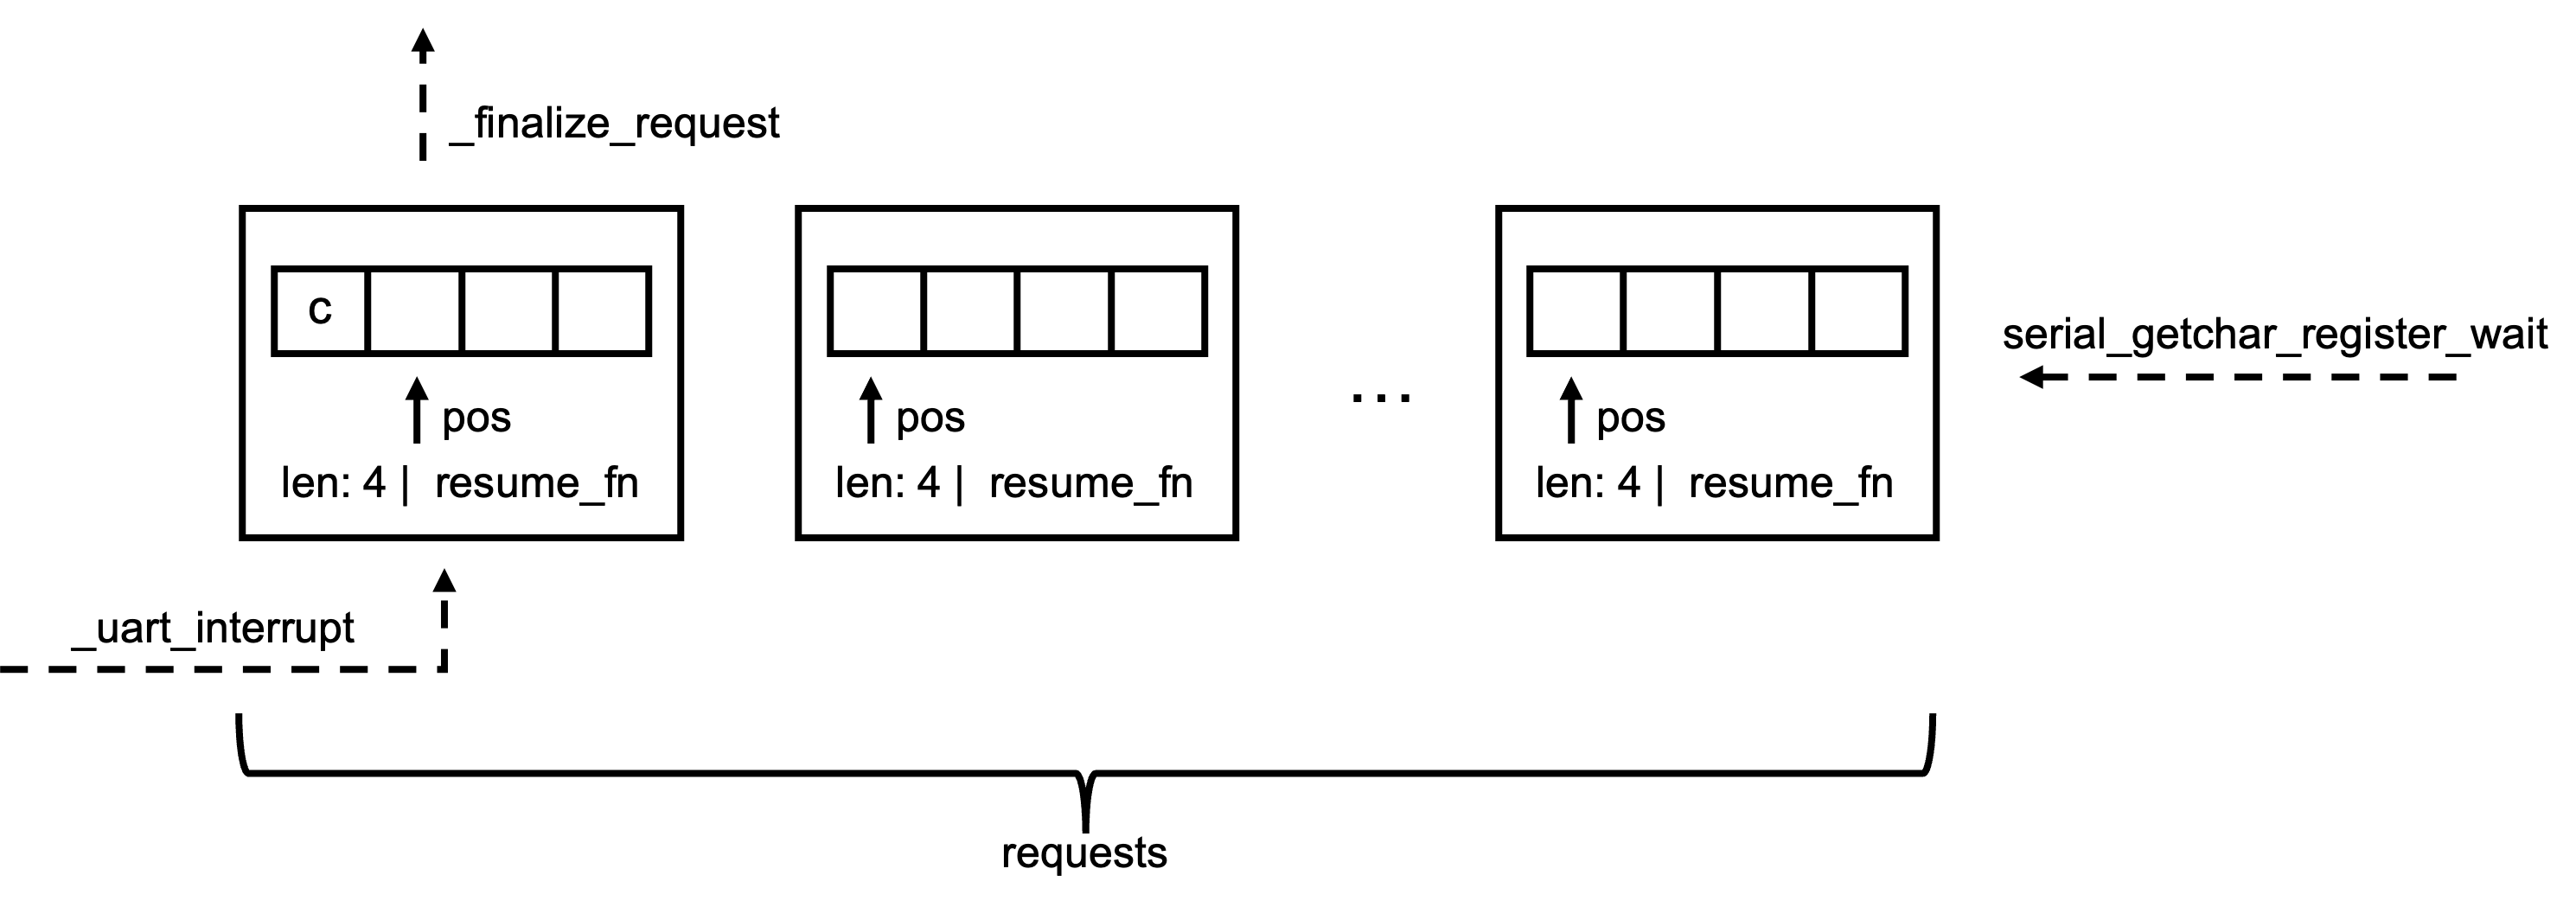
\includegraphics[width=12cm]{images/serial/serial_read.png}
    \caption{Lifetime of a \texttt{serial\_getchar\_request}}
    \label{fig:serial_read}
\end{figure}

\subsection{I/O via RPC} \label{sec:shell_io_via_rpc}

Any serial RPC calls will eventually be processed by the init process of core 0 as outlined in the introduction, potentially being relayed in case the caller is being executed on any other core. Here, the methods outlined in Listing \ref{listing:shell_serial_interface} serve as the basis for the implementation. In addition to supporting the required \texttt{aos\_rpc\_serial\_getchar}  and \texttt{aos\_rpc\_serial\_putchar} procedures, the terminal server allows the caller to read/write entire buffers using the corresponding \texttt{*\_str} functions. As the serial driver infrastructure is set up to support buffers by default, the character specific versions can be considered special cases of the more general buffer methods.

In case the serial driver was initialized with an unknown platform, the RPC calls fall back to the appropriate syscalls bypassing the need to relay to core 0. As outlined in Section \ref{sec:shell_read_uart}, \texttt{serial\_getchar\_register\_wait} is non-blocking. As previously discussed, this is required as the init process is not allowed to block in our implementation.

\subsection{Testing the Serial Server}

We evaluate the functionality of our serial server implementation by using a user process named \texttt{serial\_tester}. Initially, the \texttt{serial\_tester} performs a sequence of write operations and subsequently performs a variable number of read operations. By spawning a single instance of the \texttt{serial\_tester}, we can test the fundamental features of the serial server. However, to examine potential interleaving and ensure accurate line-based multiplexing, we spawn multiple processes for testing purposes\footnote{We can spawn multiple \texttt{serial\_tester} processes by providing the desired number of processes to spawn as a command line argument: \texttt{run serial\_tester [num\_procs]}}.

\section{Command-Line Interface}


Having discussed the technical underpinnings, we can now discuss the implementation of the shell. The shell implements a command-line interface by reading a single character at a time\footnote{A line based approach would be insufficient to support tab-competition and syntax highlighting effectively.}, tokenizing it, and finally interpreting the command. The following section covers the entire process roughly in this order, before examining the more advanced features (i.e., the extra challenge) in subsection \ref{sec:shell_pipes_and_io}. 

\subsection{Reading a Line}

The \textbf{entire code was written from scratch} as part of this project, although porting the \texttt{readline} code from the FreeBSD library or more lightweight alternatives such as \href{https://github.com/antirez/linenoise}{\texttt{linenoise}} would have been considerably more straightforward. In particular, support for cursor navigation, erasing the input, keyboard shortcuts, history, and command completion were implemented. Furthermore, the shell supports \emph{horizontal scrolling}, if the length of the current command exceeds the available width.

Shells typically read input in \textbf{raw mode} to e.g., support keyboard shortcuts, tab completion and/or syntax highlighting. As our shell supports all of these features, we read characters one at a time via the corresponding \texttt{aos\_rpc\_serial\_getchar} call, our equivalent to raw mode. \texttt{tty\_read\_skip\_multi\_byte} wraps this call and ignores any multi-byte UTF-8 characters\footnote{To significantly reduce complexity, we do not support multi-byte UTF-8 sequences.}.

As part of the \texttt{shell\_read\_line} function, the shell continuously polls for user input using the aforementioned procedure. If the polled character is printable, it is inserted into the current line at the cursor position. Otherwise, it must be handled explicitly. This includes:
% keystroke package
\begin{itemize}
	\item \texttt{KEY\_BACKSPACE} \keys{\backspace} The character at cursor position is removed;
	\item \texttt{KEY\_TAB} \keys{\tab} Tab completion is invoked via \texttt{shell\_tab\_complete}. For more details on tab completion see subsection \ref{sec:shell_tab_completion};
	\item \texttt{KEY\_ENTER} \keys{\return} The current line is flushed and \texttt{shell\_read\_line} returns. The read line is ready to be parsed and executed;
	\item \texttt{KEY\_CTRL\_C} \keys{\ctrl + C} The current line is flushed, removed from the history and the process of reading a line is restarted. In other words, any input or command is discarded, and the shell waits new input from the user;
	\item \texttt{KEY\_CTRL\_A} \keys{\ctrl + A} / \texttt{KEY\_CTRL\_E} \keys{\ctrl + E} The cursor is moved to the beginning or the end of the current line respectively;
	\item \texttt{KEY\_CTRL\_L} \keys{\ctrl + L} The terminal screen is cleared, while preserving the active line. As a result, the shell's interface is refreshed, proving a clean and blank slate for the user to continue their interactions;
	\item \texttt{KEY\_CTRL\_W} \keys{\ctrl + W} The word preceding the cursor position within the current line buffer is deleted. In other words, all characters before the cursor are removed until the first whitespace character is encountered;
	\item \keys{\arrowkeyright} / \keys{\arrowkeyleft} The cursor position is moved forward, or backward respectively\footnote{Additionally, the shell supports the alternative key combinations \texttt{KEY\_CTRL\_F} \keys{\ctrl + F} and \texttt{KEY\_CTRL\_B} \keys{\ctrl + B}.};
	\item \keys{\arrowkeyup} / \keys{\arrowkeydown} The current line is cleared and the shell displays the preceeding or succeeding command, respectively\footnote{Additionally, the shell supports the alternative key combinations \texttt{KEY\_CTRL\_P} \keys{\ctrl + P} and \texttt{KEY\_CTRL\_N} \keys{\ctrl + N}.}. The concrete implementation of the command history is detailed in subsection \ref{sec:shell_cmd_history}.
\end{itemize}


To ensure efficient performance and flexibility, the line buffer is implemented using a  \href{https://en.wikipedia.org/wiki/Gap_buffer}{\texttt{gap\_buffer}} data structure, a generalized version of the \href{https://en.wikipedia.org/wiki/Dynamic_array}{\texttt{dynamic\_array}}. This implementation enables the buffer to grow dynamically as needed and facilitates fast insertion and removal operations at any position within the buffer. By utilizing the gap\_buffer, the shell can efficiently handle command editing and tab completion on large input sizes without compromising performance. Overall, the choice of the gap\_buffer data structure provides a robust and versatile solution for managing the shell's line buffer.


\subsection{Command History}\label{sec:shell_cmd_history}

The command history is enabled by a \href{https://en.wikipedia.org/wiki/Dynamic_array}{\texttt{dynamic\_array}} storing the user's previous commands as instances of the \texttt{history\_item} struct. Once a command has been issued via the \texttt{KEY\_ENTER} \keys{\return} command, the string representing the current command is appended to the history. To enable editing past commands, each \texttt{history\_item} implements a \emph{copy-on-write} mechanism. Once the user first edits a \texttt{history\_item}, it is copied to the corresponding \texttt{gap\_buffer} on which any edits will take place. Additionally, the user's cursor position is stored per \texttt{history\_item} to enable a more pleasant editing experience.

\begin{lstlisting}[caption={Shell: Enabling Command History via the \texttt{history\_item} struct},label={listing:shell_history_item}]
struct history_item {
    bool              dirty;  ///< use buf iff. dirty
    char             *str;    ///< "committed" history
    struct gap_buffer buf;    ///< edited history

    size_t cursor;            ///< cursor into the text buffer
    size_t vcursor;           ///< cursor position on the screen
};
\end{lstlisting}

\subsection{Tab Completion}\label{sec:shell_tab_completion}

Tab completion is invoked as part of \texttt{shell\_read\_line} on \texttt{KEY\_TAB} \keys{\tab}. It works by calling the session's current \texttt{tab\_complete\_fn}\footnote{The code currently does not make use of this abstraction. Instead, the \texttt{tab\_complete} function defined in \texttt{shell.c} is called regardless of the current context.}. This function is expected to populate \texttt{shell\_tab\_complete\_results} based on the current context provided via the \texttt{struct parsed\_autocomplete} parameter. In particular, it is possible to differentiate based on the current \texttt{mode}, whether the user is in the process of completing a command, a variable or an argument. Furthermore, the struct contains a \texttt{buf} containing the token to complete, as well as the current context \texttt{ctx}. The context denotes the current command in the case of arguments and variables, and is left empty in the case of commands. The \texttt{parsed\_autocomplete} struct is populated in a specialized variant of regular command parsing, described in section \ref{sec:shell_cmd_parsing}. 
\\ \\
\smallskip 
The shell's suggestions are based on the current \texttt{mode}:
\begin{itemize}
	\item In command mode, the shell suggests completions by searching through a \href{https://en.wikipedia.org/wiki/Trie}{trie} including all the builtin commands and aliases. The entire token is considered as the prefix when looking for matching commands or aliases.
	\item Similarly, when in variable mode, the shell utilizes a trie that stores active session variables. By traversing this trie, the shell gathers potential variable matches and suggestes them as completions.
	\item In argument mode the shell currently does not provide any suggestions. It is worth noting that the implementation of argument suggestion could be realized easily.
\end{itemize}

If the returned tab completion result contains more than a single element, successive \texttt{KEY\_TAB} \keys{\tab} events cycle through the returned set by default. Otherwise the current token is substituted by the suggestion and a space is inserted\footnote{In the empty results case no substitution occurs.}. Tab completion for session variables differs slightly in the singleton case: the shell does not insert an additional whitespace. Any subsequent \texttt{KEY\_TAB} \keys{\tab} event will substitute the variable with its value.


\subsection{Command Parsing} \label{sec:shell_cmd_parsing}

While more sophisticated approaches such as a \href{https://en.wikipedia.org/wiki/Recursive_descent_parser}{Recursive Descent Parser}, or a \href{https://en.wikipedia.org/wiki/Shift-reduce_parser}{Shift-Reduce Parser} would offer more flexibility\footnote{e.g., the ability to support bracketed expressions}, the command parser is implemented as a \emph{simple state machine}. This choice was made in part because the parser must provide satisfactory results, when handling syntactically invalid commands to support both tab completion and syntax highlighting.


A simplified version of the state machine used to parse \emph{command strings} is depicted in Figure \ref{fig:shell_parser}. In particular, the depicted automaton does not handle quoted strings and escape sequences. In our implementation, however, both commands as well as arguments may be quoted and/or contain escape sequences.




\tikzset{every picture/.style={line width=0.75pt}} %set default line width to 0.75pt        

\begin{figure}[H]
\centering
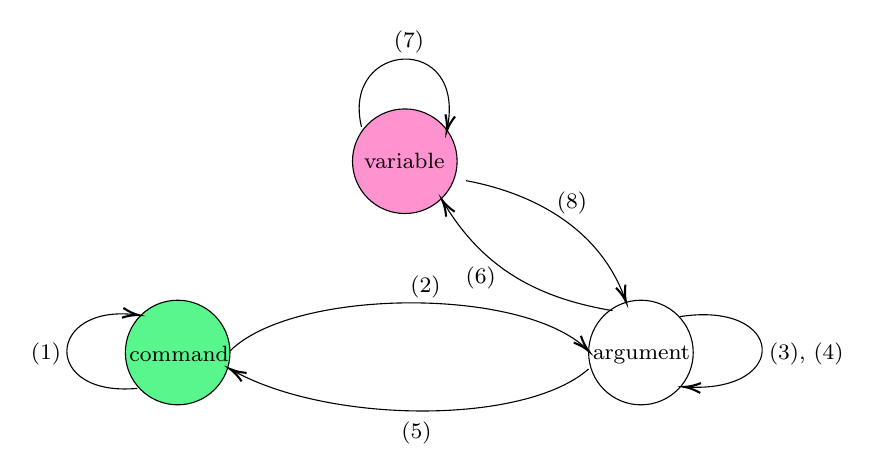
\begin{tikzpicture}[x=0.75pt,y=0.75pt,yscale=-0.72,xscale=0.72]
%Flowchart: Connector [id:dp006172763589022745] 
\draw  [fill={rgb, 255:red, 89; green, 246; blue, 142 }  ,fill opacity=1 ] (100,218) .. controls (100,198.67) and (115.67,183) .. (135,183) .. controls (154.33,183) and (170,198.67) .. (170,218) .. controls (170,237.33) and (154.33,253) .. (135,253) .. controls (115.67,253) and (100,237.33) .. (100,218) -- cycle ;
%Flowchart: Connector [id:dp9857393942850851] 
\draw   (410,218) .. controls (410,198.67) and (425.67,183) .. (445,183) .. controls (464.33,183) and (480,198.67) .. (480,218) .. controls (480,237.33) and (464.33,253) .. (445,253) .. controls (425.67,253) and (410,237.33) .. (410,218) -- cycle ;
%Curve Lines [id:da5249870829172163] 
\draw    (170,217) .. controls (212.09,174.95) and (365.4,173.55) .. (408.72,215.71) ;
\draw [shift={(410,217)}, rotate = 226.34] [color={rgb, 255:red, 0; green, 0; blue, 0 }  ][line width=0.75]    (10.93,-3.29) .. controls (6.95,-1.4) and (3.31,-0.3) .. (0,0) .. controls (3.31,0.3) and (6.95,1.4) .. (10.93,3.29)   ;
%Curve Lines [id:da1715846206115994] 
\draw    (410,229) .. controls (367.22,266.81) and (235.33,266.01) .. (170.97,229.55) ;
\draw [shift={(170,229)}, rotate = 30.03] [color={rgb, 255:red, 0; green, 0; blue, 0 }  ][line width=0.75]    (10.93,-3.29) .. controls (6.95,-1.4) and (3.31,-0.3) .. (0,0) .. controls (3.31,0.3) and (6.95,1.4) .. (10.93,3.29)   ;
%Flowchart: Connector [id:dp3515667087969462] 
\draw  [fill={rgb, 255:red, 255; green, 147; blue, 208 }  ,fill opacity=1 ] (252,90) .. controls (252,70.67) and (267.67,55) .. (287,55) .. controls (306.33,55) and (322,70.67) .. (322,90) .. controls (322,109.33) and (306.33,125) .. (287,125) .. controls (267.67,125) and (252,109.33) .. (252,90) -- cycle ;
%Curve Lines [id:da5437841267502748] 
\draw    (426,190) .. controls (379.47,182.08) and (340.78,164.36) .. (312.84,117.43) ;
\draw [shift={(312,116)}, rotate = 59.74] [color={rgb, 255:red, 0; green, 0; blue, 0 }  ][line width=0.75]    (10.93,-3.29) .. controls (6.95,-1.4) and (3.31,-0.3) .. (0,0) .. controls (3.31,0.3) and (6.95,1.4) .. (10.93,3.29)   ;
%Curve Lines [id:da24297836032951825] 
\draw    (328,103) .. controls (375.52,111.91) and (418.14,136.5) .. (434.51,182.6) ;
\draw [shift={(435,184)}, rotate = 251.2] [color={rgb, 255:red, 0; green, 0; blue, 0 }  ][line width=0.75]    (10.93,-3.29) .. controls (6.95,-1.4) and (3.31,-0.3) .. (0,0) .. controls (3.31,0.3) and (6.95,1.4) .. (10.93,3.29)   ;
%Curve Lines [id:da2798236433090334] 
\draw    (108,242) .. controls (43.65,247.94) and (46.93,185.27) .. (107.16,192.75) ;
\draw [shift={(109,193)}, rotate = 188.26] [color={rgb, 255:red, 0; green, 0; blue, 0 }  ][line width=0.75]    (10.93,-3.29) .. controls (6.95,-1.4) and (3.31,-0.3) .. (0,0) .. controls (3.31,0.3) and (6.95,1.4) .. (10.93,3.29)   ;
%Curve Lines [id:da15564769244860654] 
\draw    (258,67) .. controls (244.07,9.29) and (329.14,3.06) .. (315.22,69) ;
\draw [shift={(315,70)}, rotate = 282.62] [color={rgb, 255:red, 0; green, 0; blue, 0 }  ][line width=0.75]    (10.93,-3.29) .. controls (6.95,-1.4) and (3.31,-0.3) .. (0,0) .. controls (3.31,0.3) and (6.95,1.4) .. (10.93,3.29)   ;
%Curve Lines [id:da0016551100974000477] 
\draw    (471,194) .. controls (541.65,183.05) and (545.96,245.37) .. (475.07,241.07) ;
\draw [shift={(474,241)}, rotate = 3.97] [color={rgb, 255:red, 0; green, 0; blue, 0 }  ][line width=0.75]    (10.93,-3.29) .. controls (6.95,-1.4) and (3.31,-0.3) .. (0,0) .. controls (3.31,0.3) and (6.95,1.4) .. (10.93,3.29)   ;

% Text Node
\draw (101,212) node [anchor=north west][inner sep=0.75pt]   [align=left] {{\footnotesize command}};
% Text Node
\draw (411,212) node [anchor=north west][inner sep=0.75pt]   [align=left] {{\footnotesize argument}};
% Text Node
\draw (258,83) node [anchor=north west][inner sep=0.75pt]   [align=left] {{\footnotesize variable}};
% Text Node
\draw (35,210) node [anchor=north west][inner sep=0.75pt]  [font=\normalsize] [align=left] {{\footnotesize (1)}};
% Text Node
\draw (289,165) node [anchor=north west][inner sep=0.75pt]   [align=left] {{\footnotesize (2)}};
% Text Node
\draw (529,210) node [anchor=north west][inner sep=0.75pt]   [align=left] {{\footnotesize (3), (4)}};
% Text Node
\draw (283,263) node [anchor=north west][inner sep=0.75pt]   [align=left] {{\footnotesize (5)}};
% Text Node
\draw (387,109) node [anchor=north west][inner sep=0.75pt]   [align=left] {{\footnotesize (8)}};
% Text Node
\draw (326,159) node [anchor=north west][inner sep=0.75pt]   [align=left] {{\footnotesize (6)}};
% Text Node
\draw (278,1) node [anchor=north west][inner sep=0.75pt]   [align=left] {{\footnotesize (7)}};
\end{tikzpicture}
\caption{Simplified Version of the State Machine used for Command Parsing} \label{fig:shell_parser}
\end{figure}

Operating on a single character at a time, we handle the following transitions as part of the simplified command parsing (see Figure \ref{fig:shell_parser}):
\begin{itemize}
	\item \textbf{(1)}, \textbf{(3)}, \textbf{(7)} Read the current character and append it to the respective buffer, implemented as a \texttt{dynamic\_array}.
	\item \textbf{(2)} If the current character is a whitespace, we append the contents of the command buffer to the set of commands and start reading arguments.
	\item \textbf{(4)} A whitespace character denotes the end of an argument. Therefore, we append the contents of the argument buffer to the list of arguments, and begin parsing of the next argument.
	\item \textbf{(6)} If the current character denotes the beginning of a variable, i.e., equals \texttt{'\$'}, we treat successive characters as part of a variable.
	\item \textbf{(8)} Once the end of a variable has been detected, typically be a whitespace character, we look up the contents of the variable buffer in the trie storing active session variables.
	\item \textbf{(5)} If the current character represents an operator, e.g., \texttt{|}, \texttt{;}\footnote{For two character operators, e.g., \texttt{\&\&} and \texttt{||}, we may need to peek at the next character.}, it denotes the end of an argument list and the start of a succeeding command. Therefore, we append the current argument to the set of arguments of the current command and the operator to the list of operators.
\end{itemize}


Our implementation builds upon the simplified state machine, additionally checking for quoted strings and escape sequences as part of the \texttt{command} and \texttt{argument} states. As a result of performing this parsing stage, we obtain a parsed list of commands, including arguments and the delimiting operators. The parsed command line is stored in a \texttt{struct parsed\_command\_pipeline}:

\begin{lstlisting}[caption={Shell: Enabling Command History via the \texttt{history\_item} struct},label={listing:shell_parsed_cmd_pipeline}]
/// struct storing a single command within a pipeline
struct parsed_command {
    char  *command;
    size_t argc;
    char **argv;
};
/// entire parsed command pipeline, consisting of multiple commands
struct parsed_command_pipeline {
    size_t                 size;
    struct parsed_command *cmds;
    char                  *ops;  ///< (size-1) delimiting operators
    char                  *err_str;
};
\end{lstlisting}

\texttt{cmdparse.c}  also includes variations of the outlined function that support tab completion and syntax highlighting. However, from a conceptual standpoint, both procedures closely resemble the outlined methodology. The main difference lies in the actions carried out during each transition.

\subsection{Session Variables}\label{sec:shell_session_vars}

\newcommand{\ShellVar}[1]{{\color{shell_variable}\texttt{#1}}}

The shell automatically stores the PID (\ShellVar{\$!}) and the exit code (\ShellVar{\$?}) as variables when executing commands\footnote{\ShellVar{\$?} is only set when spawning applications in the foreground}. For any \emph{builtin}, the stored PID variable corresponds to the PID of the shell, whereas the \ShellVar{\$!} variable reflects PID of the spawn process in the case of an \emph{alias}. See section \ref{sec:shell_builtin} for the difference between the two.

In addition to implementing the required \ShellVar{\$?} and \ShellVar{\$!} variables, the shell supports arbitrary user defined variables. Variables are declared using \texttt{bash} syntax\footnote{Variables cannot be declared as part of a command, and must be declared a single variable at a time.}:

\begin{lstlisting}[style=ShellInputStyle]
 +~$+ @my_var@=42
 define: my_var := '42'
\end{lstlisting}

declares a variable named \texttt{my\_var} and sets its value to $42$. After having defined the variable, it can be used via the \ShellVar{\$my\_var} syntax:


\begin{lstlisting}[style=ShellInputStyle]
 +~$+ echo "my_var has the value @$my_var@"
 my_var has the value 42
\end{lstlisting}

Currently, it is not possible to declare variables as part of a command, or to declare multiple variables in a single line.

Internally, all active session variables are stored in a trie. This allows variables to be inserted/updated efficiently, while simultaneously serving as the foundation for their tab completion.

\begin{figure}[htp]
    \centering
    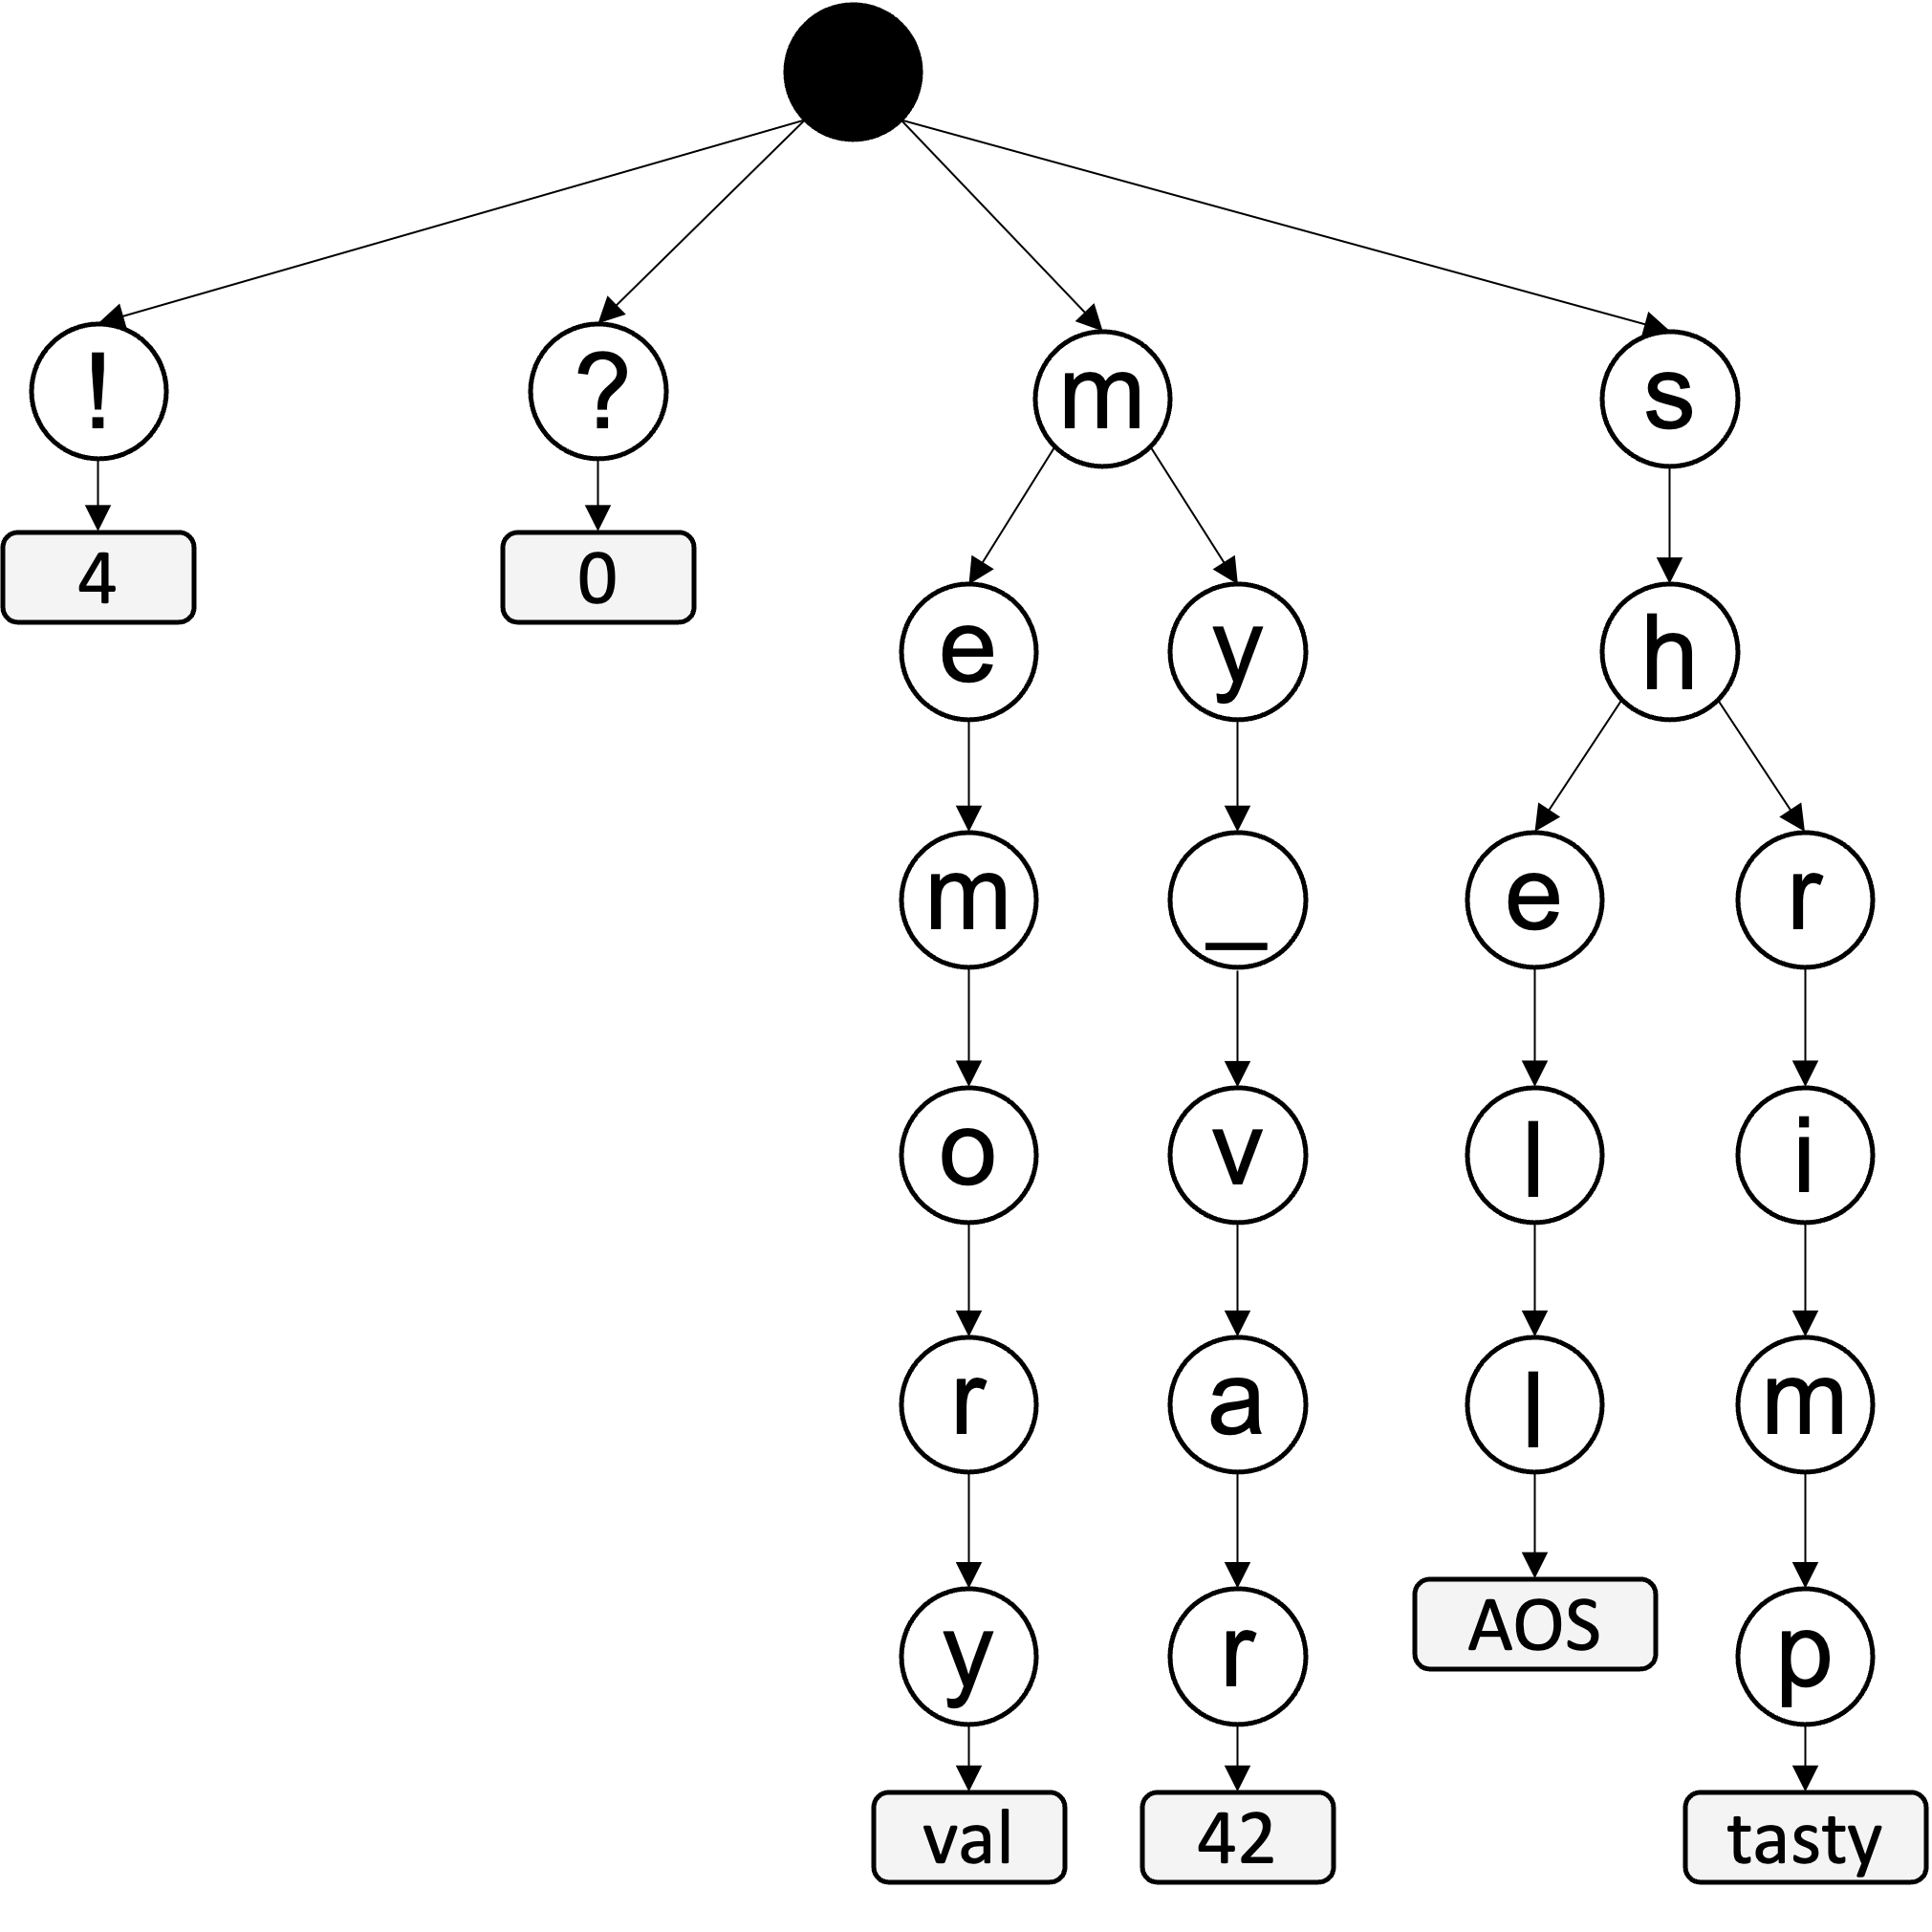
\includegraphics[width=6.5cm]{images/shell/var_trie.png}
    \caption{Trie Storing Active Session Variables}
    \label{fig:shell_var_trie}
\end{figure}

Note that variables are substituted as part of the \emph{parsing stage}. This implies that the following are semantically different:

 \begin{lstlisting}[style=ShellInputStyle]
 +~$+ run hello
 +~$+ echo @$!@
\end{lstlisting}

runs the \texttt{hello} application and outputs its process identifier (PID), whereas

 \begin{lstlisting}[style=ShellInputStyle]
 +~$+ run hello +;+ echo @$!@
\end{lstlisting}

runs the \texttt{hello} application and outputs the preceeding process' PID, i.e., the one we would have obtained by running \texttt{echo \$!} directly.

\begin{comment}
	maybe think about mentioning that they are "implicitly quoted" (i.e., count as a single argument) 
\end{comment}

\subsection{Syntax Highlighting}\label{sec:shell_syntax_highlighting}

Syntax highlighting in a shell is essential as it enables users to visually differentiate elements within a single line of input, such as commands, variables, and operators. This distinction significantly improves productivity and enhances the user experience. Similar to tab completion, syntax highlighting builds upon a specialized variant of the parsing stage, in this case: \texttt{\_pst\_color\_char}.

As part of the aforementioned function, the shell populates a \href{https://en.wikipedia.org/wiki/Dynamic_array}{\texttt{dynamic\_array}} of \texttt{cmdline\_color\_t}s. Each \texttt{cmdline\_color\_t} constitutes of a starting position \texttt{begin} and a buffer storing the color to apply, encoded using \href{https://en.wikipedia.org/wiki/ANSI_escape_code}{ANSI escape codes}. When refreshing the current line, the shell respects the constructed array of colors, by applying them in the correct order. As supporting syntax highlighting requires additional line refreshes, it is possible to disable syntax highlighting via the corresponding \texttt{SHELL\_CMDLINE\_COLORS} macro.

\begin{lstlisting}[style=ShellInputStyle]
 +~$+ echo "syntax %*\shellquote* highlighting @$rocks@" +>+ §out.txt§
\end{lstlisting}

As every character potentially requires a line refresh with syntax highlighting, we experimented with refreshing the line on every input. This occasionally causes blinking. Thus, in the current implementation the shell refreshes the line only upon processing \emph{special characters}, e.g.,  whitespaces and  operators.


\section{Shell Builtins} \label{sec:shell_builtin}

Thoughtful consideration has been given to designing the way command are defined in order to facilitate the implementation of a wide range of functionalities within the shell. The excerpt of \texttt{cmdbuiltins.h} shown in Listing \ref{listing:shell_cmd_define} explains how commands are defined within the shell. Specifically, defining commands as part of the macro ensures that they are listed in the \texttt{help} command, the corresponding \texttt{man} pages are populated, and that the commands are inserted into the command trie.

\begin{lstlisting}[caption={Shell: Defining \texttt{BUILTIN}s and \texttt{ALIAS}es as Part of the Shell},label={listing:shell_cmd_define}]
#define CMD_BUILTIN_FOREACH(BUILTIN, ALIAS) 	                 \
   BUILTIN(man, CMD_BUILTIN_GROUP_BASIC, _cmd_builtin_man,     \
	         "display a manual pages", "man <builtin>", NULL)    \
   ALIAS(echo, CMD_BUILTIN_GROUP_BASIC,                        \
         "writes the first argument to standard output",       \
         "echo <message>", "[...]")                            \
   [...]\end{lstlisting}

For an exhaustive list of all implemented commands, we refer to the User Guide of Appendix Section \ref{sec:appendix_user_guide}.

As Listing \ref{listing:shell_cmd_define} indicates, the shell differentiates between \emph{builtin}s and \emph{alias}es. A builtin is executed \emph{as part of} the shell, whereas an \emph{alias} is delegated to a seperate process.  For example, executing the alias \texttt{echo} can be considered equivalent to executing \texttt{run echo}.

In most cases, this distinction is not visible to the user. For \emph{command pipelines}, as discussed in section \ref{sec:shell_pipes_and_io}, this difference is important. In particular, any command defined as a builtin cannot appear as part of a command pipeline\footnote{\texttt{BUILTIN}s may still appear within a list of commands.}. This limitation is a result of the way I/O redirection is implemented: we would have to redirect the shell's input/output, or handle this case explicitly.

\begin{comment}
	TODO: mention launching a "shell within a shell"
\end{comment}

\subsection{The \texttt{time} Utility}

The \texttt{time} utility measures the time taken to execute another command. As we want to support timing the execution of command pipelines and list of commands, \texttt{time} is neither implemented as a \texttt{BUILTIN} nor as an \texttt{ALIAS}\footnote{Technically speaking, we provide a \texttt{time} builtin for the purpose of detecting illegal use, populating \texttt{help}, and the corresponding \texttt{man} page.}. Instead, the shell explicitly checks if the parsed list of commands starts with a \texttt{time} directive. In this case, the shell initiates timed execution of the entire set of commands, as depicted in Listing \ref{listing:shell_time_ex}.

\begin{lstlisting}[style=ShellInputStyle, caption={Timing the Execution of a List of Commands}, deletekeywords={echo, command}, label={listing:shell_time_ex}]
 +~$+ time echo "first command" +;+ !echo! "second command"
 first command
 second command
 %took: 0m:0.218s% (real)
\end{lstlisting}

\subsection{Process Management}

The shell provides numerous commands to allow the user to effectively manage processes, e.g., \texttt{kill}, \texttt{pause}, \texttt{resume}, and \texttt{ps}. Most importantly, however, the shell facilitates spawning processes via the \texttt{run <command> [\&]} and \texttt{oncore <core\_id> <command> [\&]} builtins. 

Both builtins spawn the requested process in the foreground by default, and support spawning the background via an optional trailing \texttt{\&}. Additionally, \texttt{oncore} supports spawning a process on a specific core, as specified via the required \texttt{core\_id} argument.


Spawning a process in the foreground is rather straightforward. The shell simply calls \texttt{proc\_mgmt\_spawn\_program\_argv}\footnote{Technically, it uses a variant discussed in subsequent chapters.} to spawn the process with the parsed parameters and sets \ShellVar{\$!}. Subsequently, it waits for completion of the newly spawn process by invoking \texttt{proc\_mgmt\_wait}. At this point, it is able to set the resulting \ShellVar{\$?} variable.

In contrast, spawning a process in the background is slightly more complex. The shell cannot wait for termination, and thus does not set the  \ShellVar{\$?} variable. Additionally, the shell must prevent the spawned application from consuming console input. Building upon the infrastructure set in place to support I/O redirection, the shell does this by mapping an empty frame as the process' standard input, while preserving its standard output. This means that any application spawned in the background may still print to the console as expected. Specifics related to the implementation of \emph{overriding} a process' standard in- and output are detailed in section \ref{sec:shell_pipes_and_io}.

\subsection{Filesystem}


The filesystem, a fundamental component of any operatating system, is crucial for organizing, storing, and accessing data. The shell uses this component to facilitate effective file management and navigation.

The shell stores the working directory as part of the current session. This allows builtins to operate on relative, as opposed to solely absolute, paths. To support relative paths within \texttt{ALIAS}es, the shell supplies the current working directory via a dedicated \texttt{-\phantom{}-wd} flag when spawning the associated process.

In the upcoming section, it will become evident that the shell heavily relies on the versatile \texttt{tee} alias/program to facilitate I/O redirection to files. By accepting multiple file names as command line arguments, \texttt{tee} effectively duplicates its standard input to those files.  Moreover, when \texttt{tee} is executed without the \texttt{-s} option, it further prints its standard input to the standard output (\texttt{stdout}).

To enhance functionality, we offer support for automatically suggesting file and directory names within the current directory as an experimental feature. To activate this feature, you can enable the \texttt{SHELL\_TAB\_COMPLETE\_FILENAMES} macro in the \texttt{shell.h} file.

\section{Extra Challenge: Pipes and I/O Redirection} \label{sec:shell_pipes_and_io}

While it is already useful to spawn an individual process, the use of the shell becomes substantially more effective when it starts to orchestrate sets of command pipelines. In particular, \href{https://en.wikipedia.org/wiki/Pipeline_(Unix)}{Unix Pipelines} offer a highly valuable abstraction for this purpose. In the following, we explore the implementation of command pipelines and their role in constructing \emph{lists of commands}.
\subsection{Command Pipelines}

A pipeline is a powerful concept in which processes are interconnected, forming a chain through their standard input and output streams. This arrangement allows the output of each process (\texttt{stdout}) to be seamlessly passed as input (\texttt{stdin}) to the next process. It is important to note that all the processes within a pipeline are executed concurrently, thereby enhancing efficiency and enabling faster execution. Listing \ref{listing:shell_pipeline_ex} provides an example of a pipeline evaluation.

\begin{lstlisting}[style=ShellInputStyle, deletekeywords={command}, caption={Execution of an Exemplary Pipeline}, label={listing:shell_pipeline_ex}]
 +~$+ echo "something to pipeline across process'" | wc
       1       5      38
\end{lstlisting}

The shell also supports redirecting a process' output via \texttt{>}. To unify both types of redirection any use of \texttt{>} is \emph{desugared}, making use of the \texttt{tee} alias. E.g., the statement

\begin{lstlisting}[style=ShellInputStyle, deletekeywords={command}]
 +~$+ echo "my very long string" +|+ wc -l +>+ §foo.txt§
\end{lstlisting}
is translated into
\begin{lstlisting}[style=ShellInputStyle, deletekeywords={command}]
 +~$+ echo "my very long string" +|+ wc -l +|+ tee foo.txt -s
\end{lstlisting}

wherein the trailing \texttt{-s} is appended in case the respective file redirection is the last command within the current pipeline. Otherwise, it is omitted. This allows pipelines to contain multiple successive file redirections, e.g.,
\begin{lstlisting}[style=ShellInputStyle, deletekeywords={command}]
 +~$+ echo "very important message" +>+ §file1.txt§ +>+ §file2.txt§
\end{lstlisting}
or after \emph{desugaring}
\begin{lstlisting}[style=ShellInputStyle, deletekeywords={command}]
 +~$+ echo "very important message" +|+ tee file1.txt +|+ tee file2.txt -s
\end{lstlisting}
in which case both \texttt{file1.txt} and \texttt{file2.txt} will be populated. This follows naturally, as \texttt{tee} additionally replicates its input to \texttt{stdout} if \texttt{-s} is ommited. Thus, the second \emph{desugared} \texttt{tee} will be passed the duplicated input.

After \emph{desugaring}, the shell must, therefore, only facilitate the seamless flow of standard streams through a series of successive processes. This functionality is built on top of User-Level Message Passing (UMP). To enable pipelines, the following generalization of \texttt{spawn\_load\_with\_caps} was introduced:

\begin{lstlisting}[caption={Generalization of \texttt{spawn\_load\_with\_caps}}]
errval_t spawn_load_mapped(struct spawninfo *si,
	struct elfimg *img, int argc, const char *argv[], int capc,
	struct capref caps[], domainid_t pid, struct capref stdin_frame,
	struct capref stdout_frame);\end{lstlisting}

While accepting mostly the same arguments as \texttt{spawn\_load\_with\_caps}, the caller is able to provide additional \texttt{stdin\_frame} and \texttt{stdout\_frame} parameters. These frames are emplaced into the newly constructed process' \texttt{CSpace} at well-known locations: \texttt{TASKCN\_SLOT\_STDIN\_FRAME} and \texttt{TASKCN\_SLOT\_STDOUT\_FRAME} respectively.

Both slots are checked as part of the thread initialization performed in \texttt{barrelfish\_init\_onthread}. If the slots are populated appropriately, a UMP endpoint is initialized using the passed frame. Subsequent reads/writes now make use of the corresponding UMP functions. If a frame is not initialized, reads/writes rely on the standard rpc functionality as described in section \ref{sec:shell_io_via_rpc}. This logic is encapsulated in the \texttt{iox} library. The libc function pointers are set up to make use of this abstraction:

\begin{lstlisting}[caption={}]
_libc_terminal_read_func  = iox_read;
_libc_terminal_write_func = iox_write;\end{lstlisting}

To orchestrate a pipeline, the shell makes use of the rpc \emph{wrapper} of this function, \texttt{aos\_rpc\_proc\_spawn\_mapped}. First, the shell allocates a sufficient number of frames\footnote{For a pipeline of length $n$, the shell allocates $n - 1$ frames.} and then spawns the requested programs, providing the corresponding in- and output frames. This mapping is visualized in Figure \ref{fig:shell_pipes}. After having spawned all processes, the shell waits for their completion.

\begin{figure}[htp]
    \centering
    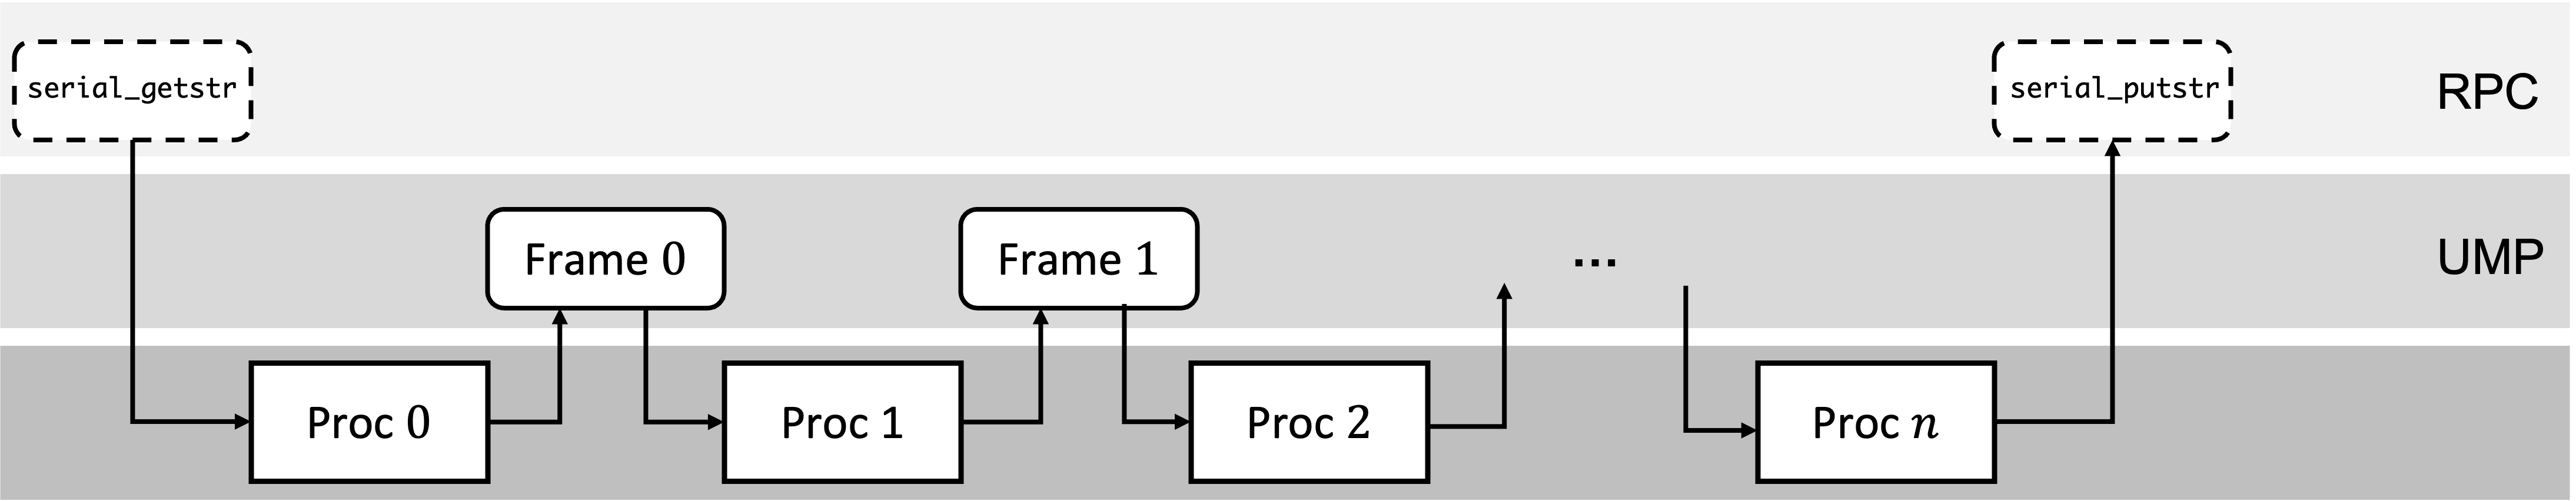
\includegraphics[width=12cm]{images/shell/shell_pipes.png}
    \caption{Pipeline orchestrated by the Shell}
    \label{fig:shell_pipes}
\end{figure}

The way pipelines are constructed, any command that is part of a pipeline\footnote{of size at least two} must be an \texttt{ALIAS} and not a \texttt{BUILTIN}. As any command within the pipeline must, consequently, refer to a separate program, the user may omit the \texttt{run} / \texttt{oncore} tokens\footnote{However, it remains perfectly valid to keep them}. This is illustrated in Listing \ref{listing:shell_pipeline_omit}.

\begin{lstlisting}[style=ShellInputStyle, deletekeywords={run, command, wc, echo}, caption={Pipelines with or without the \texttt{run}/\texttt{oncore} Directives}, label={listing:shell_pipeline_omit}]
 +~$+ !run! echo "commands can be executed with run" | !run! wc -l
      1       6      34
 +~$+ !echo! "commands can be executed without run" | !wc! -l
      1       6      37
\end{lstlisting}

Furthermore, the operating system supports sending capabilities across cores, as detailed in chapter \ref{chapter:distcap}. Therefore, pipelines can naturally be used to facilitate arbitrary communication between processes across cores:

\begin{lstlisting}[style=ShellInputStyle, deletekeywords={run, command, wc, echo}]
 +~$+ !oncore! 1 echo "hello from the other core..." | !oncore! 0 wc
      1       5      29
\end{lstlisting}


 Note that a process can still perform explicit printing and reading operations to the terminal using the corresponding RPC calls. We discussed the possibility of introducing a permission system, allowing processes to be spawned with a limited set of permitted operations. However, in the end, we chose not to implement such a mechanism.

\subsection{Lists of Commands}

Similar to bash, our shell supports \href{https://www.gnu.org/software/bash/manual/html_node/Lists.html}{Lists of Commands}. A list of commands consists of one or more pipelines arranged in a specific order, with each pipeline separated by one of the following operators: \texttt{;}, \texttt{\&\&}, or \texttt{||}. 

Mutliple pipelines within a list of commands are not run concurrently. Instead, pipelines are executed sequentially one after another, potentially short-circuiting based on the exit code:
\begin{itemize}
	\item \texttt{;} No short-circuiting is applied. The exit code corresponds to the last executed command pipeline.
	\item \texttt{\&\&} If the previous pipeline returned an exit code \texttt{!= 0}, execution ends immediately, returning the preceding pipeline's exit code
\begin{lstlisting}[style=ShellInputStyle, deletekeywords={run, command, wc, echo}]
 +~$+ true +&&+ !echo! "short-circuiting example"
 short-circuiting example
 +~$+ false +&&+ !echo! "short-circuiting example"
\end{lstlisting}
	\item \texttt{||} If the previous pipeline returned an exit code \texttt{== 0}, execution ends immediately, with the exit code $0$.
\begin{lstlisting}[style=ShellInputStyle, deletekeywords={run, command, wc, echo}]
 +~$+ true +||+ !echo! "short-circuiting example"
 +~$+ false +||+ !echo! "short-circuiting example"
 short-circuiting example
\end{lstlisting}
\end{itemize}

Futhermore, pipelines are always executed from left to right, i.e., all operators delimiting pipelines \texttt{;}, \texttt{\&\&}, \texttt{||} have the same operator precedence. This significantly simplifies parsing, while adhering to the bash specification. Currently, there is no way to group commands.

\section{Limitations}

As described in the previous sections, the shell supports a large number of features, from syntax highlighting and tab completion to I/O redirection and pipes. Building upon the existing capabilities, there are several potential avenues to further improve the functionality of the shell:
\bigbreak
\textbf{Interleaving between \texttt{debug\_printf} and \texttt{printf}} Debug output printed as part of a \texttt{debug\_printf} may be interleaved with output of the serial server. This is a consequence of \texttt{debug\_printf} relying on the corresponding \texttt{SYSCALL}, which in turn accesses the UART driver directly. To prevent such an interleaving, we may call the serial server for \texttt{debug\_printf}, or write debug output to a dedicated file.
\bigbreak
\textbf{Improved Syntax Highlighting} The current version of syntax highlighting could be extended to correctly display the \texttt{time} primitive, to highlight the command argument passed to \texttt{run}/\texttt{oncore}, or to highlight files.
\bigbreak
\textbf{Support for \texttt{BUILTIN}s in Command Pipelines} One limitation of our command pipelines is that they do not support running \texttt{BUILTIN}s. Instead, only an alias/binary may be run from within a pipeline. It may be worthwhile to consider adding support \texttt{BUILTIN}s, by spawning them in a separate process, or by having the shell populate the relevant I/O frames.
\bigbreak
\textbf{Tab completion for Command Arguments} Tab completion for command arguments is already supported in theory, as demonstrated by the support for auto-completing filenames. In addition, it could be implemented for the most common \texttt{BUILTIN}s/\texttt{ALIAS}es. In particular, we may consider implementing tab completion for the first argument of \texttt{run}, i.e., the program to execute.
\bigbreak
\textbf{Permissions for Mapped Processes} In our current implementation, any process is able to print and read from the terminal via the UART by explicitly calling the corresponding RPC calls. One might extend our solution by implementing a permission system, so that this is no longer possible.
\bigbreak
\textbf{General Purpose Working Directory} Instead of using the \texttt{\-\phantom\-wd} flag to provide the current working directory when launching a process associated with an alias like \texttt{ls} or \texttt{tee}, an alternative approach could be to offer a general purpose function to retrieve the current working directory. This would enable processes to access and retrieve the working directory when they are launched using \texttt{run} or \texttt{oncore}. 

\section{Retrospective}

Working on this milestone was a challenging and simultaneously rewarding journey. By implementing the entire shell from the ground up, I have considerably improved my understanding of the whole stack: from the intricacies of dealing with I/O, as part of \texttt{readline} and implementing fundamental data structures such as tries and gap buffers, to the efficient transfer of data between processes using piping.

As this task took considerable amounts of time, sweet, and tears, I would \emph{certainly} recommend to instead port the readline code from \texttt{FreeBSD} libraries, as helpfully pointed out in the book.	
\chapter[Filesystem]{Filesystem \\ \Large \textnormal{François Costa}}

\section{Overview of the architecture}

\begin{itemize}
    \item \textbf{fopen.c}: This file represents the high-level library and is the inteface with other processes, facilitating their interaction.

    \item \textbf{aos\_rpc.c}: Serves as a bridge between the high-level library and the FAT32 filesystem, this file handles the communication between shared libraries and FAT32. It ensures the maintenance of invariants enforced by the disk.

    \item \textbf{fat32.c}: Is responsible for the implementation of the FAT32 filesystem, this file provides the necessary services to maintain the required invariants.

    \item \textbf{blockdriver.c}: Is acting as the block driver, this file handles the actual communication with the disk, serving as a vital component of the overall system.

    \item \textbf{fat32\_test.h}: During the compile time, this header-only file, which serves the purpose of testing the filesystem, is incorporated into \texttt{fat32.c}. This file isn't present in the production code.

\end{itemize}

The initial section provides an overview of the high-level architecture used for the implementation. In the filesystem implementation, several files assume significant roles:
 
\begin{figure}[htp]
    \centering
    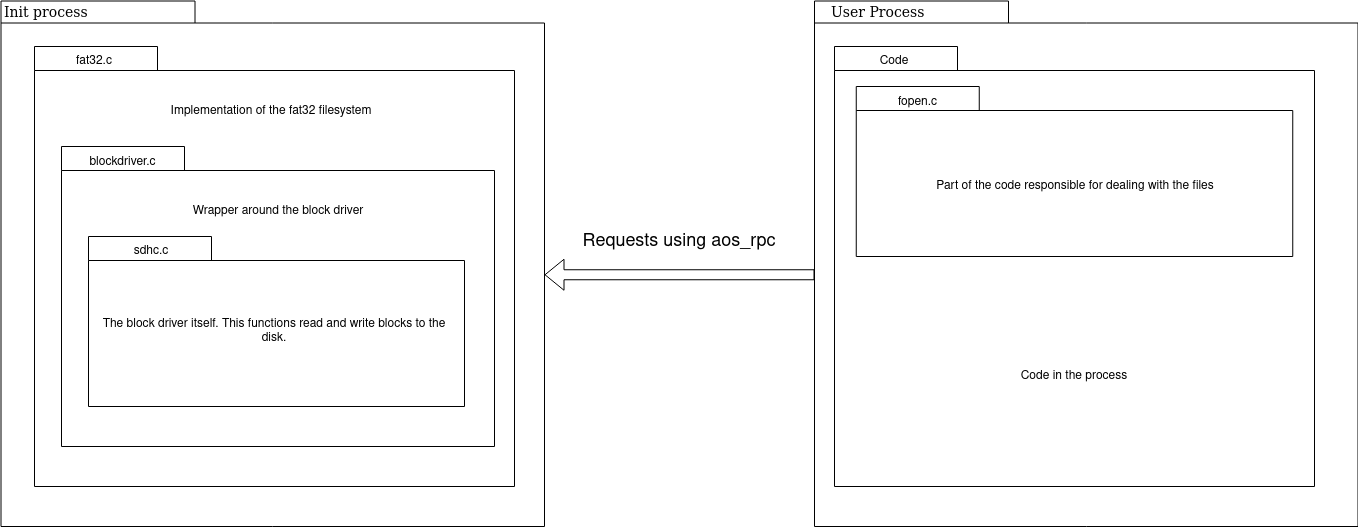
\includegraphics[width=12cm]{images/filesystem/high_level overview.drawio.png}
    \caption{High level overfiew of the architecture}
    \label{fig:galaxy}
\end{figure}


\subsection{Each module has its own scope}
In the system architecture, each C file holds specific responsibilities. We can make a clear distinction between them. The block driver communicates with the disk, ensuring smooth data transfer. The FAT32 filesystem focuses on maintaining the necessary invariants required by the filesystem itself. Lastly, the RPC framework takes charge of communication between the system and external entities, providing a way to interact with the rest of the world.

\subsection{The block driver and the filesystem are bound together}

An architectural decision that is very important is the \textbf{coexistence} of the block driver and the FAT32 filesystem within the same process (init), eliminating the need for RPC (Remote Procedure Call) communication between them. The filesystem holds a pointer to the driver block, enabling direct communication with the disk. While the filesystem assumes the responsibility of \textbf{maintaining the disk's invariants}, the block driver handles the actual \textbf{disk communication}. Both components operate within the init process as part of a larger system-wide design paradigm. By consolidating all services within init and directing all RPC requests to it, this design choice aligns with the overall system architecture (see LMP section for more details). Consequently, the filesystem architecture follows the notion of not reinventing the wheel, utilizing existing components efficiently.

This architectural decision was carefully made to ensure \textbf{consistency} across the entire system. Maintaining consistency is important as it promotes coherence, predictability, and compatibility among different components and processes within the system.

\subsection{The filesystem maintains the required invariants in a fat32 filesystem}

At the core of this architecture lies a core concept: establishing a \textbf{singular point of trust} for maintaining the essential invariants required by the FAT32. This responsibility rests solely with the internal workings of the FAT32 itself, which effectively utilizes the block driver to establish communication with the disk. As a consequence, any request pertaining to the filesystem must follow a prescribed path, traversing through the init process and, more specifically, the FAT32 filesystem component (\texttt{fat32.c}). This design ensures a \textbf{centralized} and controlled approach to filesystem operations, reinforcing reliability and security.

The FAT32 assumes the crucial role of being the sole entity we rely on to uphold the necessary invariants within the disk. It becomes the singular point of trust, responsible for maintaining the integrity and consistency of the filesystem. By placing our trust in the FAT32, we ensure that all required invariants are preserved, providing confidence in the reliability and stability of the disk.

\subsection{Finally, a solid test infrastructure}

The file fat32\_test.h plays a crucial role in our system as it serves as the central place for executing all unit tests. Its responsibility lies in ensuring the \textbf{integrity} and functionality of various components within the system. Whenever a new feature is added or a function is modified, leveraging the tests becomes a valuable practice. These tests act as a safety net, allowing us to validate that the changes made do not introduce unforeseen issues or regressions into the system. Running the tests following a modification or addition helps ensure that the system continues to operate smoothly and as intended.

After successfully validating a set of tests, I extracted a subset from them and designed a new process to replicate the same operations. While the decision to reuse the same tests may appear unconventional, there exists a logical rationale behind it. Employing different tests could potentially unveil additional scenarios to verify, but in the event of an error, it becomes challenging to discern whether it originates from inter-process communication or the FAT32 itself. By utilizing identical tests, we expedite the bug detection process, as the high probability lies within the RPC layer. This approach significantly accelerates bug discovery, enabling prompt resolution and debugging of the system.

\begin{lstlisting}[caption={Unit tests executed},captionpos=b,language=C,frame=single,breaklines]
void _test_name_len(void);
void _test_extension_len(void);
void _test_name_valid(void);
void _test_compare_entries_call(const char *name_entry, const char *extension_entry, const char *name, bool expect);
void _test_compare_entries(void);
void _test_shortname_to_name(void);
void _test_name_to_shortname(void);
void _test_resolve_call(struct fat32_filesystem *fs, const char *test_name, const char *path, bool result);
void _test_resolve(struct fat32_filesystem *fs);
void _test_fopen(struct fat32_filesystem *fs, const char *path);
void _test_freadseek(struct fat32_filesystem *fs, const char *path);
void _test_fwrite(struct fat32_filesystem *fs, const char *path);
void _test_fwrite_huge(struct fat32_filesystem *fs, const char *path);
void _test_mk_rm(struct fat32_filesystem *fs, const char *dir);
void _test_create_write_remove(struct fat32_filesystem *fs, const char *path);

\end{lstlisting}

\section{The block driver}

\subsection{Technical background}

A block driver is a software component that enables a computer's operating system or processes to communicate with block devices, such as hard drives, solid-state drives, USB flash drives and SD cards.

A block device is a storage device that reads and writes data in fixed-size chunks or blocks. The block driver acts as an interface between the operating system and the block device, allowing the operating system to read and write data to the device. In our case, thanks to the block driver we can see our block device as a gigantic array with each entry as an array of 512 bytes.

The block driver provides a set of functions that allow the operating system to access the block device, including functions to read and write blocks of data, query device properties, and perform other operations. In addition to providing basic access to the block device, block drivers also provide functionality such as caching, buffering, and error handling. Caching and buffering can help improve performance by reducing the number of disk accesses needed to read or write data, while error handling can help ensure data integrity by detecting and correcting errors that occur during data transfer. Caching was implemented as extra challenge.

The driver block we are given is not as powerful and does not have all the features, but it allows to read and write blocks, and this is enough to build a filesystem on top of it. However, caching was implemented as extra challenge.

\subsection{Implementation of the bloc driver}

I have written a file named \texttt{blockdriver.c} that serves as an easy wrapper around the block driver. Within this file, three distinct functions were create to enhance its functionality. Firstly,  a straightforward function that initializes the blockdriver, ensuring its proper setup. Secondly, we have a function dedicated to retrieving blocks of data from the disk, which greatly aids in efficient data retrieval. Finally, the last function within this file is specifically designed to facilitate reading data from the disk, thereby streamlining the reading process. It is worth mentioning that despite its concise length, this implementation showcases no remarkable or peculiar features, as it predominantly serves as a wrapper around the provided bloc driver.

\begin{lstlisting}[caption={Wrapper around the block driver},captionpos=b,language=C,frame=single,breaklines]
struct block_driver {
    struct capref sdhc_cap;
    lvaddr_t sdhc_vaddr;

    struct capref rw_frame;
    lvaddr_t write_vaddr;
    lvaddr_t read_vaddr;
    lpaddr_t write_paddr;
    lpaddr_t read_paddr;

    struct sdhc_s *driver_structure;
};

errval_t launch_driver(struct block_driver *b_driver);

errval_t read_block(struct block_driver *b_driver, int lba, void *block);
errval_t write_block(struct block_driver *b_driver, int lba, void *block);

\end{lstlisting}

\subsection{Performance evaluation}

For the performance evaluation section, I have added two additional functions that handle reading and writing data from the provided block driver, while also measuring the time it takes to complete these operations. There is no magic involved in these functions; they simply start a timer when the reading or writing process begins and stop it once the function finishes its task.

To gauge the actual speed of the block driver, I conducted 500 read operations and 500 write operations for \texttt{benchmarking} purposes. The results are represented in two plots, which display the statistical distribution of the duration, measured in \textbf{microseconds}, for both block writes and block reads. We can see that the result is consistent with some outliers.

\begin{figure}[htp]
    \centering
    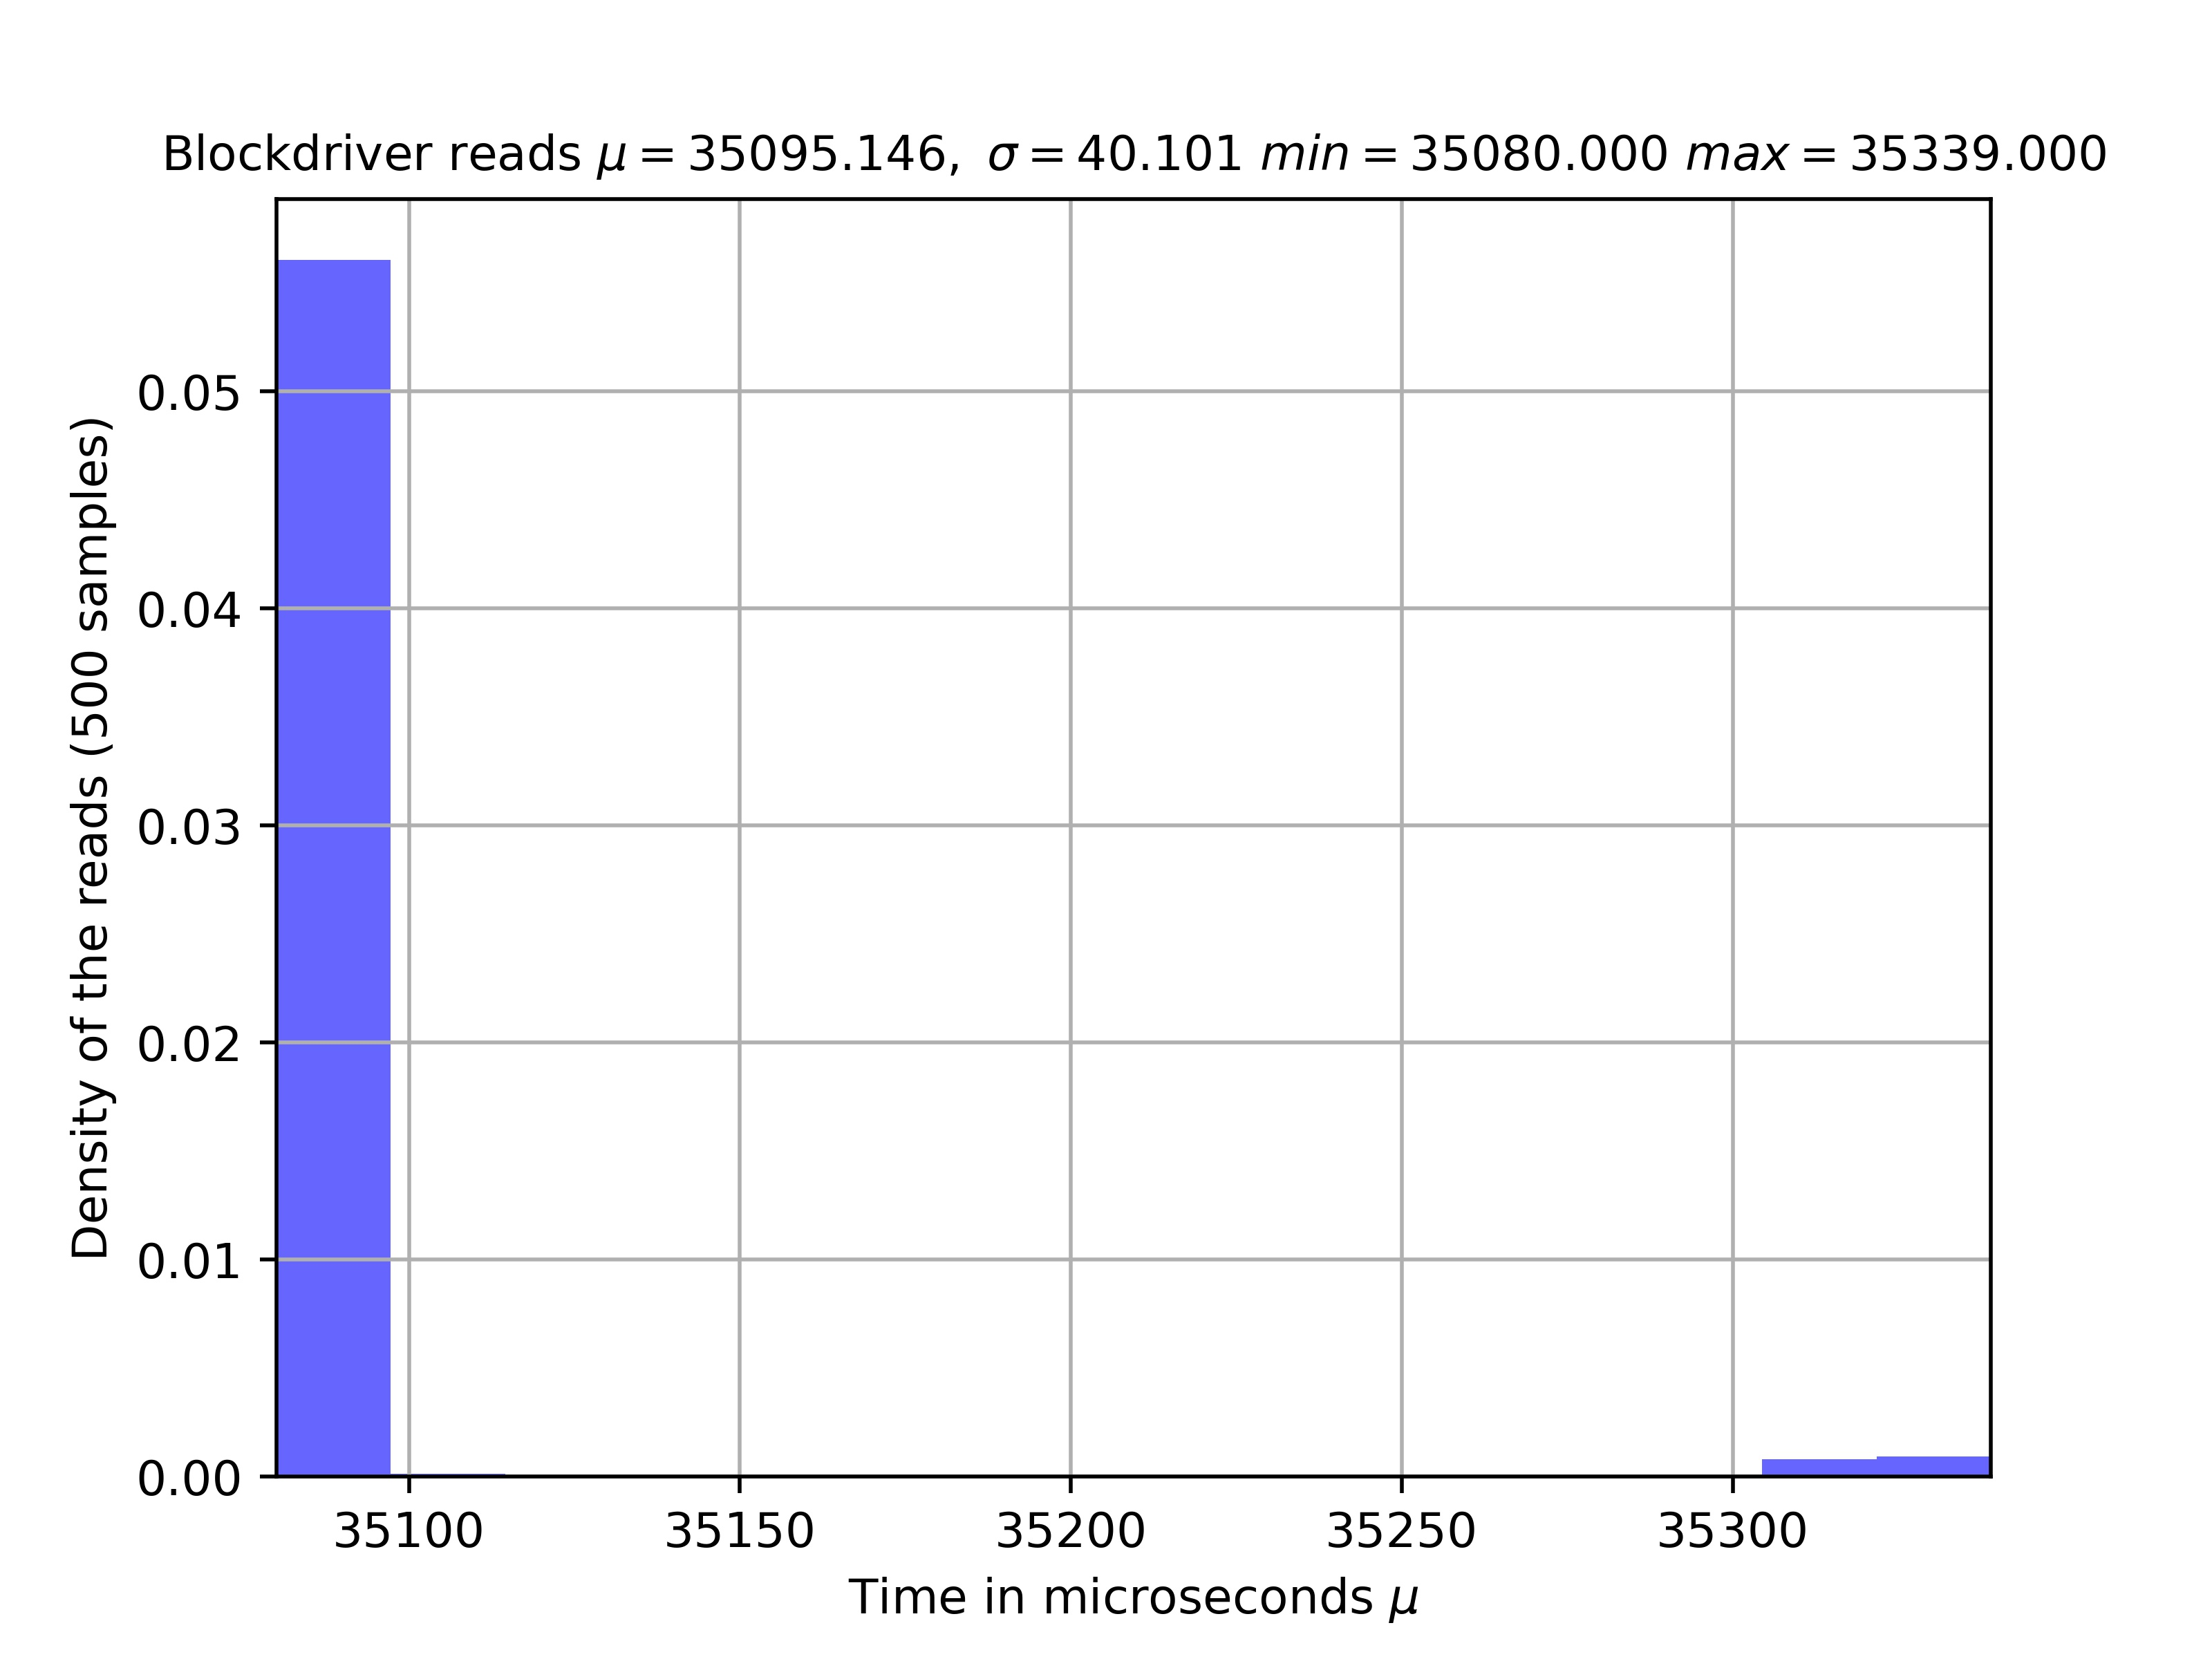
\includegraphics[width=12cm]{images/filesystem/benchmark_read.jpg}
    \caption{Benchmark blockdriver read}
    \label{fig:galaxy}
\end{figure}


\begin{figure}[htp]
    \centering
    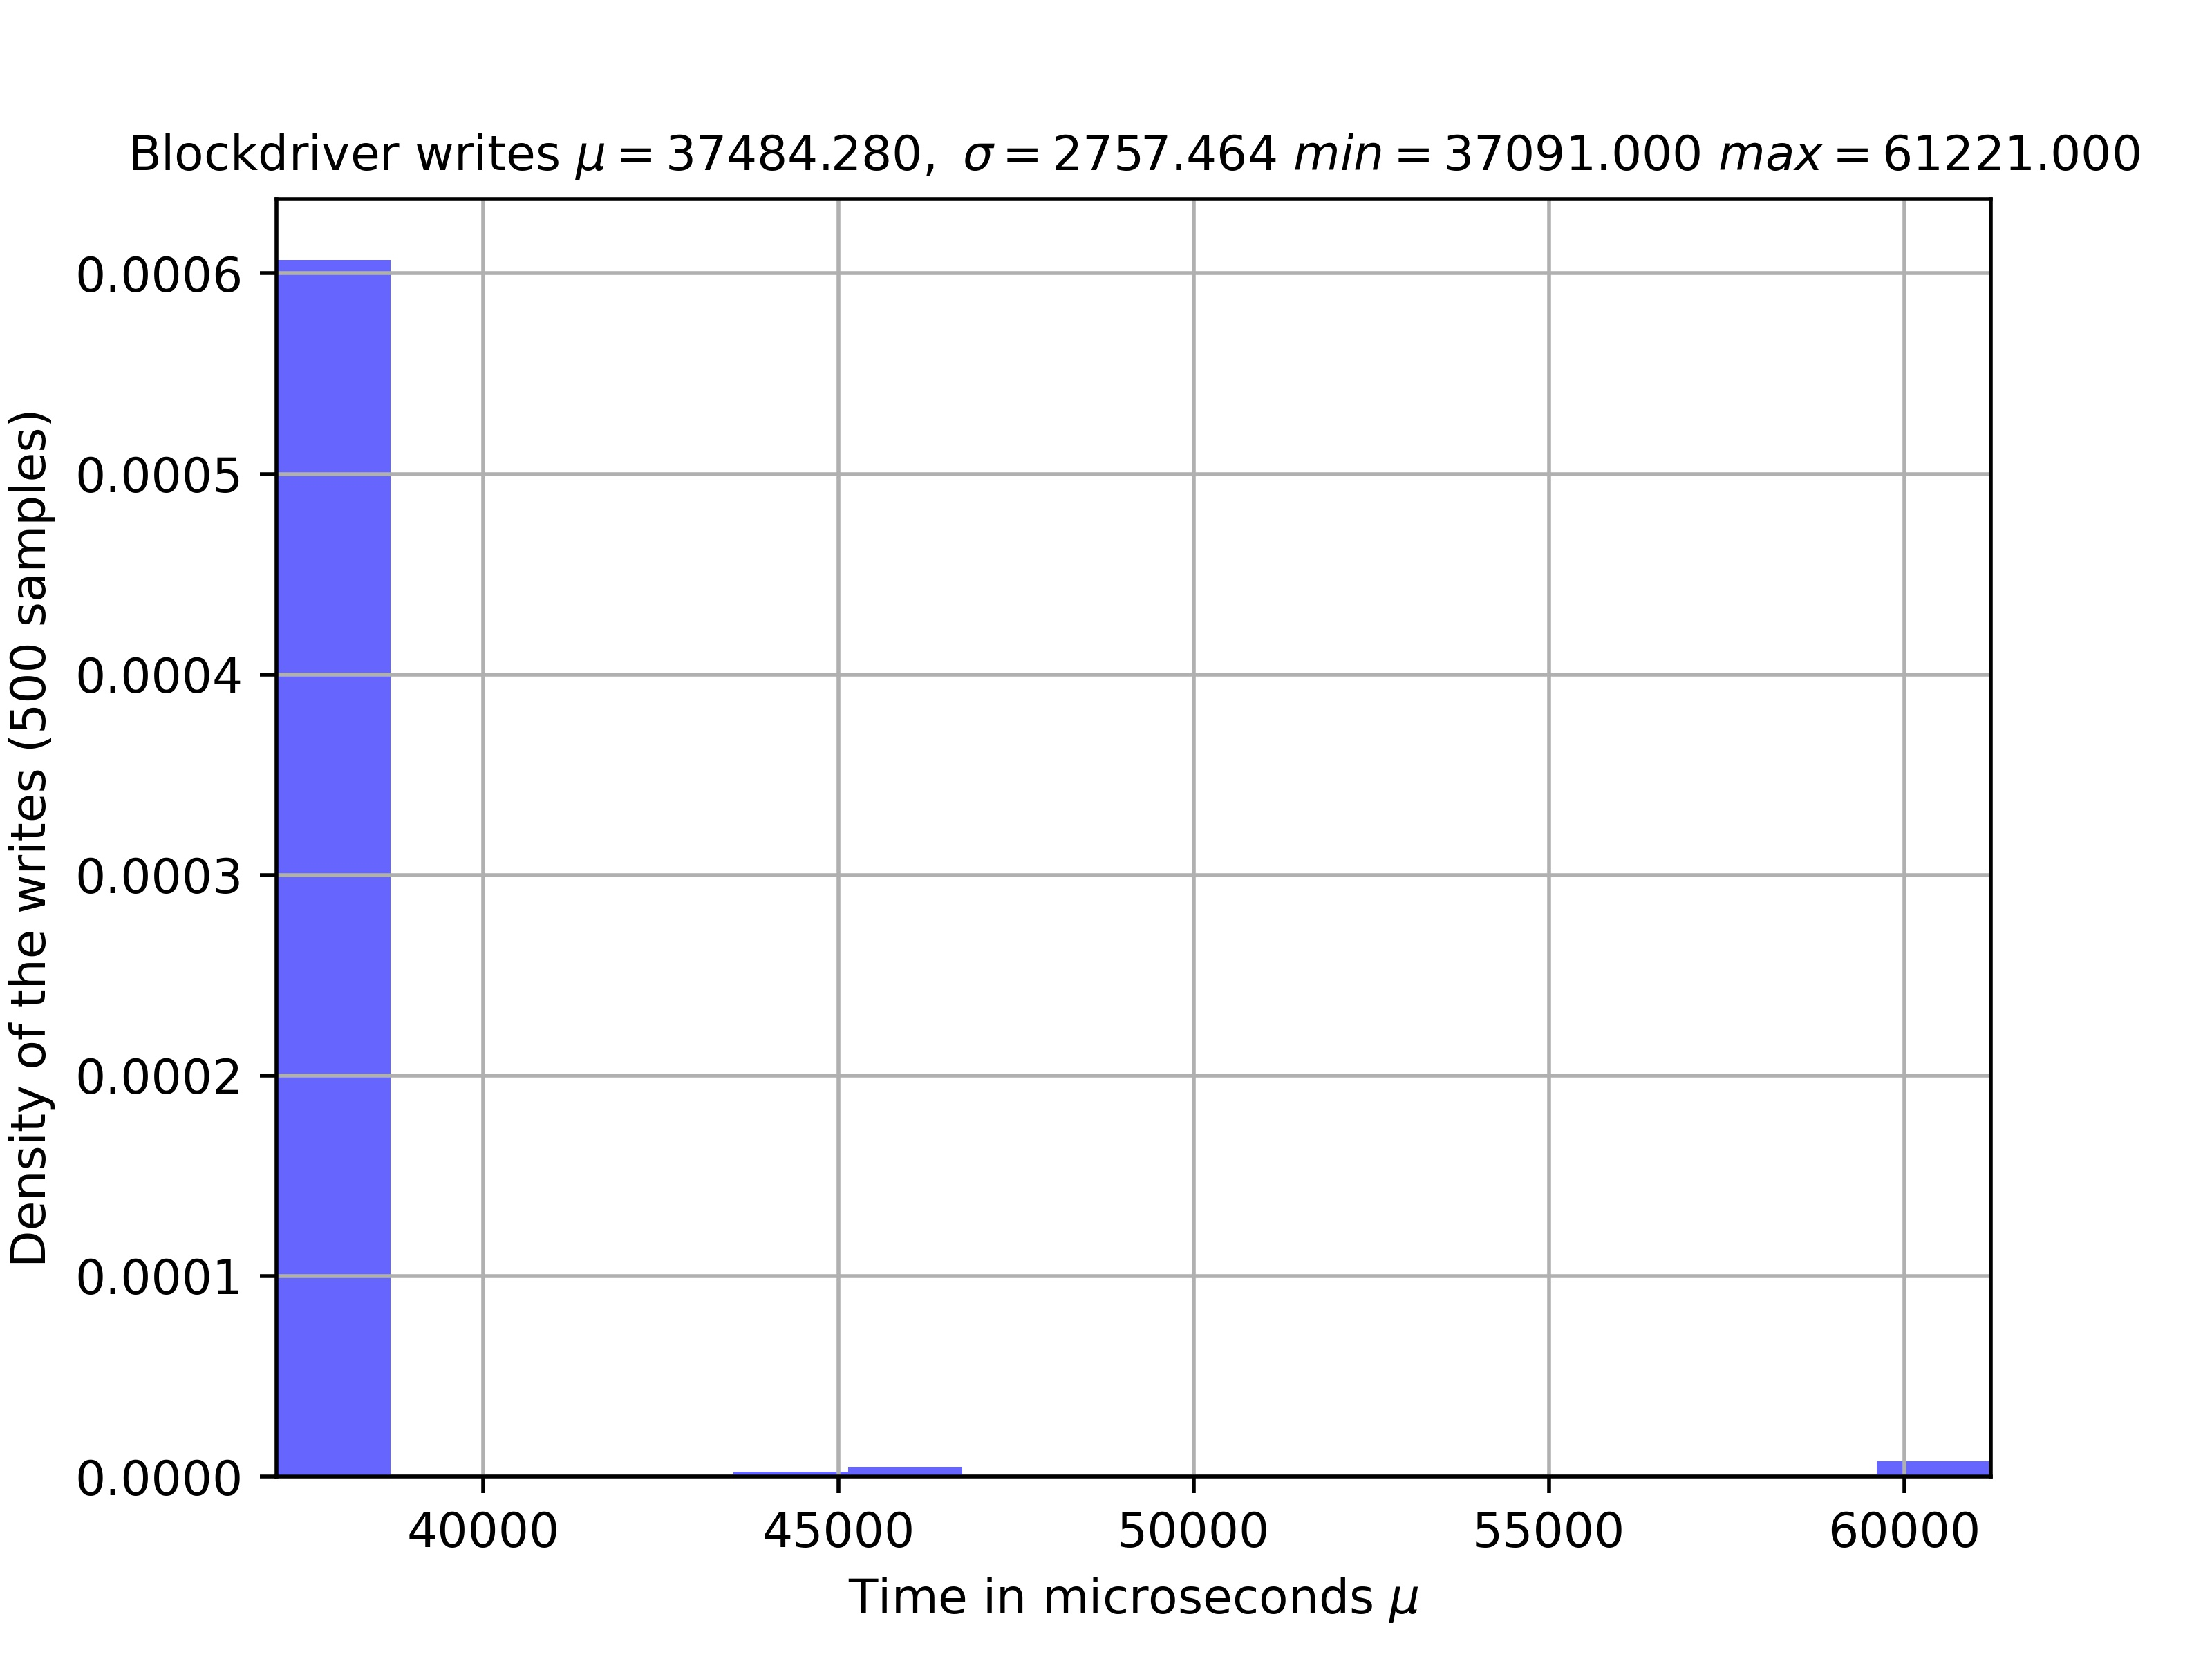
\includegraphics[width=12cm]{images/filesystem/benchmark_writes.jpg}
    \caption{Benchmark blockdriver write}
    \label{fig:galaxy}
\end{figure}

\begin{figure}[htp]
    \centering
    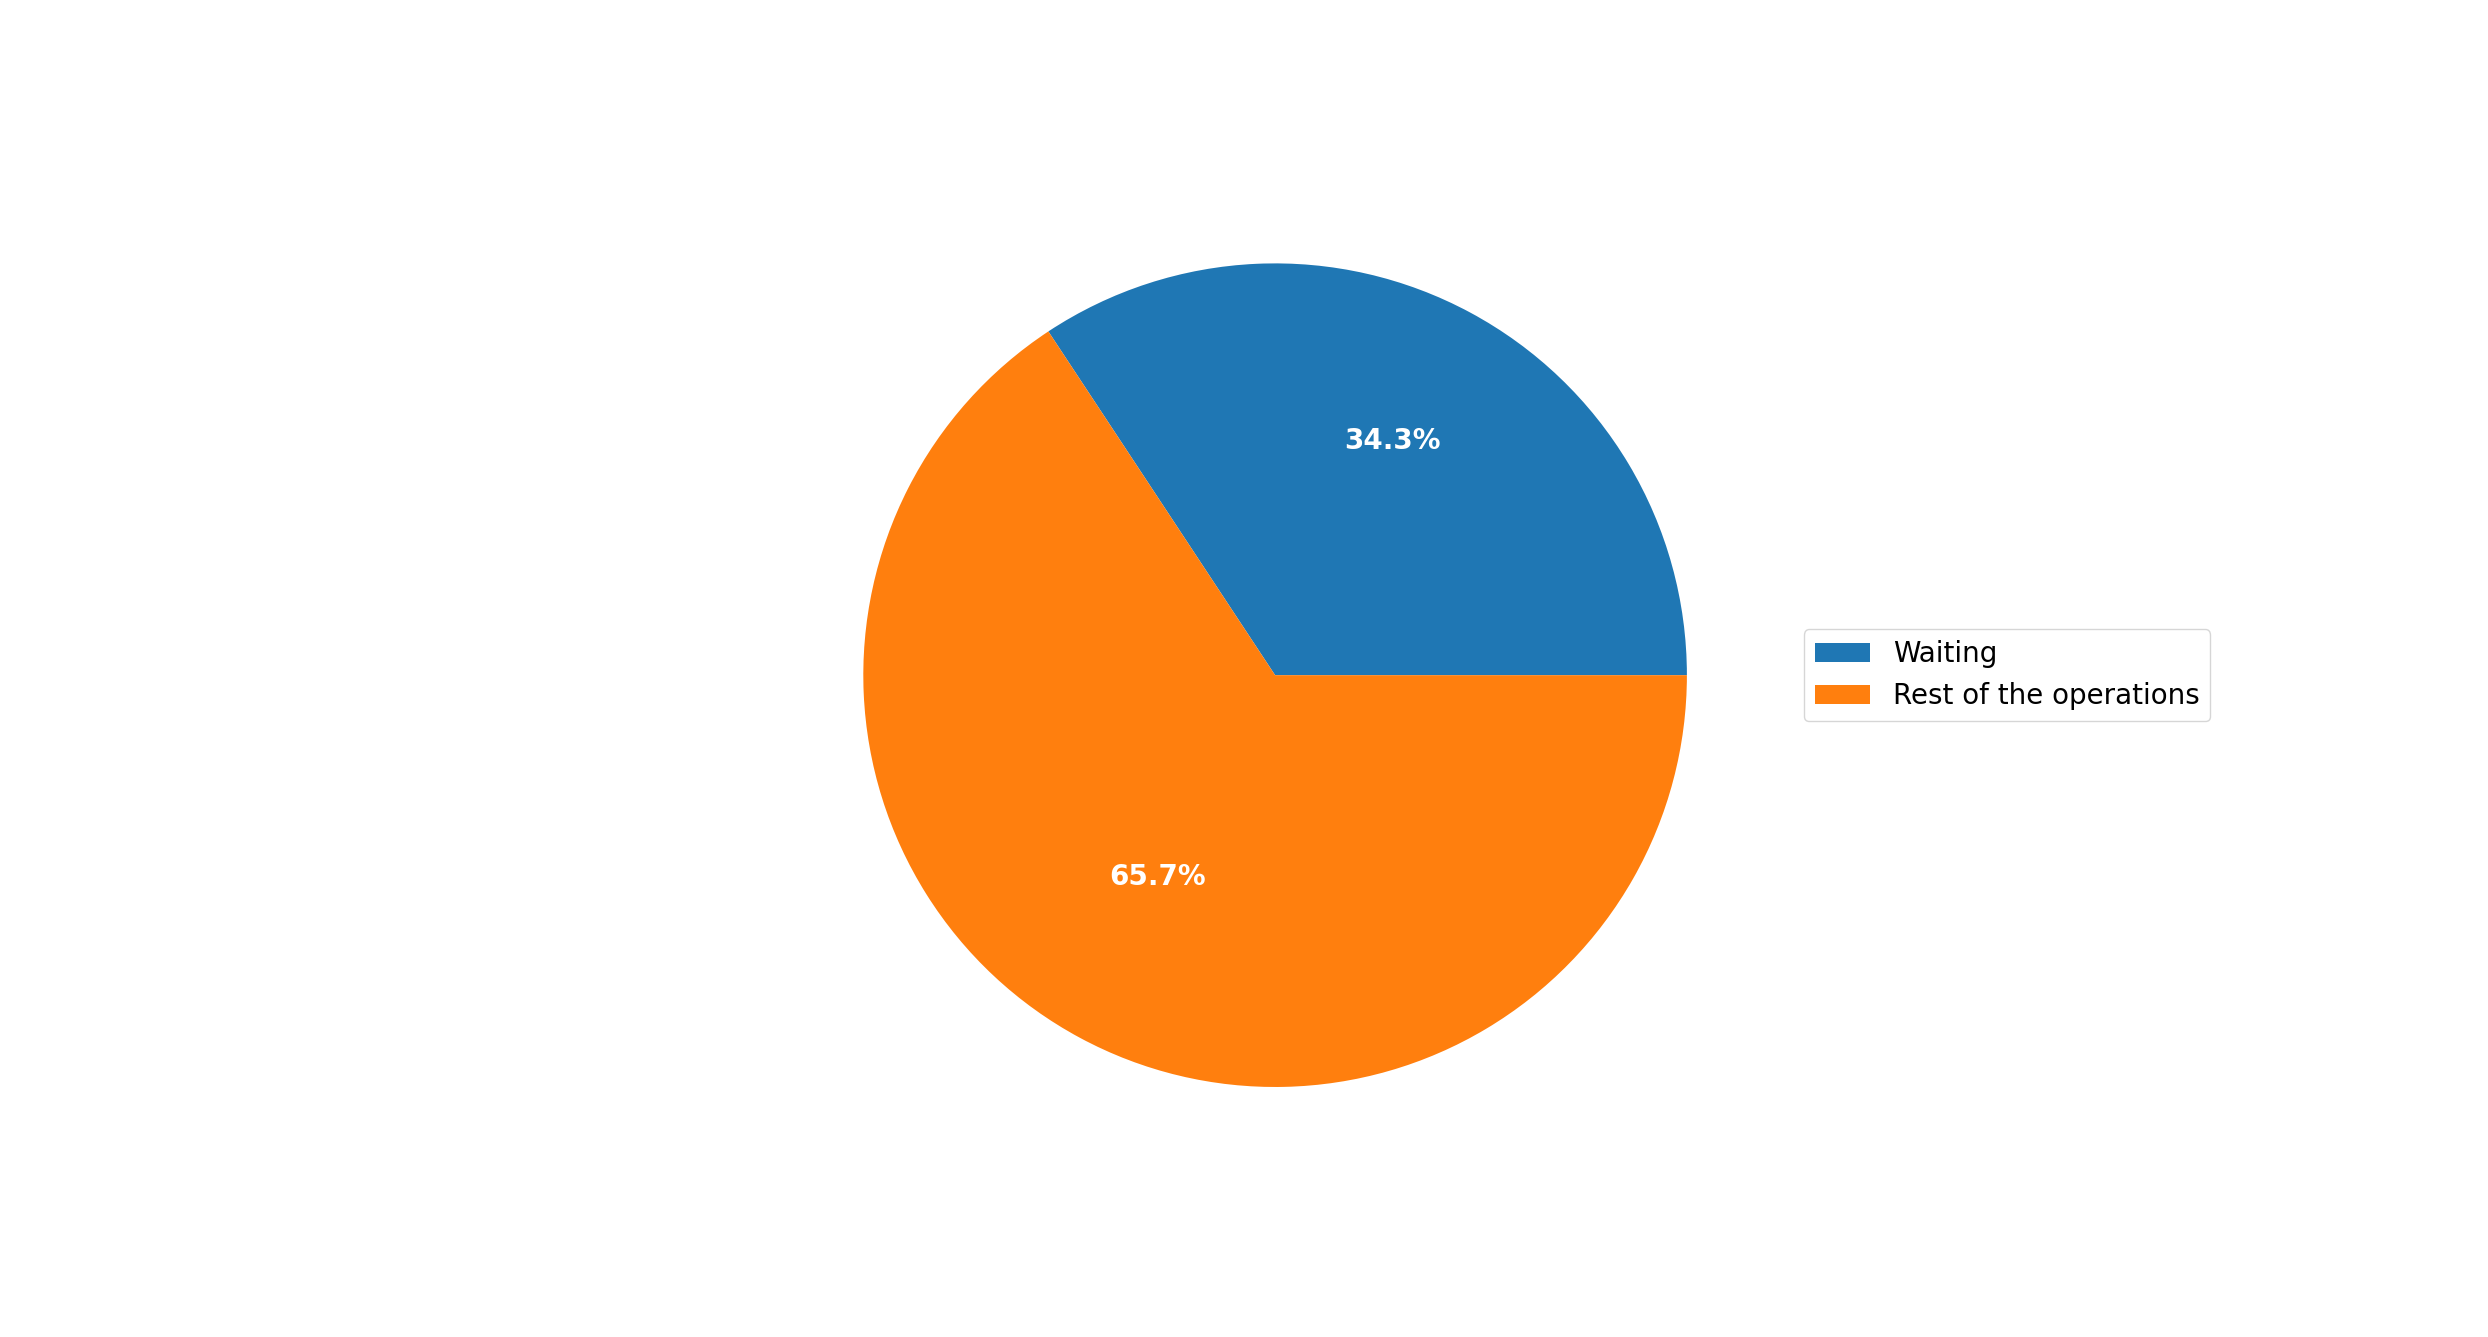
\includegraphics[width=12cm]{images/filesystem/division.png}
    \caption{Time spent in the block driver}
    \label{fig:galaxy}
\end{figure}


\subsection{Extra milestone: Implementing a \href{https://en.wikipedia.org/wiki/Cache_(computing)}{\texttt{software cache}} in the block driver}

When executing the block driver, we observe an interesting yet unsurprising pattern. The \texttt{access pattern} for blocks identified by logical block addressing (LBA) is not random at all. For instance, the \texttt{root cluster} is accessed frequently as it needs to be read each time a path in the filesystem is resolved (further explanations will be provided in the report). In technical terms, this implies the presence of \textbf{temporal locality} in the access patterns, meaning that \textbf{recently accessed elements are likely to be accessed again in the future}.

What does this signify? We are aware that reading from and writing to the disk is exceptionally slow. In the graph displayed below, you can observe the time it takes for these operations. If two blocks are similar, it would be advantageous to find an algorithm or technique to access them only once. As evident from the benchmark results, a computer can accomplish a significant amount of tasks within this time frame. Therefore, it is apparent that we are expending a considerable amount of resources needlessly. To address this issue, we will employ a mechanism known as a \texttt{software cache}.

A \texttt{software cache}. is a mechanism used in computer systems to improve performance by storing frequently accessed data or instructions closer to the processing unit. It acts as a temporary storage area between the CPU and main memory, holding copies of data that are likely to be needed again in the near future. When the CPU requests data, the cache is checked first, and if the data is found, it is retrieved from the cache, which is faster than accessing the main memory. This helps reduce the overall access time and improves system responsiveness by reducing the number of slower memory accesses required.

\begin{lstlisting}[caption={Wrapper around the driver},captionpos=b,language=C,frame=single,breaklines]
void load_driver() {
    // Setup the base driver
    init_driver();
    
   	// Init software cache
    init_cache();  
}

void read_block(size_t lba, void *block) {
    if(try_read_from_cache(lba, block)) {
      return; // Cache hit
    }

    // I/O from disk
    driver_read(lba, block);

    // Update software cache
    update_cache(lba, block);

    return;
}

void write_block(size_t lba, void *block) {
	// Invalidate cache
    invalidate_cache(lba);
  
    // Write-back
    driver_write(lba, block);
  
    return;
}
\end{lstlisting}

Considering the cache size, a cache of size 512 would likely provide better overall performance compared to a cache size of 2048 (current). Increasing the cache size allows for more data to be stored closer to the processor, potentially reducing the frequency of cache misses and improving execution speed. However, further investigation and testing are necessary to determine the optimal cache size for specific workloads.

Regarding the eviction policy, while \href{https://en.wikipedia.org/wiki/Cache_replacement_policies}{\texttt{LRU}} (Least Recently Used) is commonly used and generally effective, it may not always be the best choice for every scenario. Other eviction policies, such as LFU (Least Frequently Used) or Random, may yield better results depending on the specific access patterns and workload characteristics. Determining the ideal eviction policy would require more exploration and experimentation. The cache implements a LRU eviction policy.

Additionally, it's worth noting that the implemented cache follows a \texttt{write-through} policy, meaning that write operations are directly propagated to the main memory. While a \texttt{write-back} cache, which stores modified data in the cache itself before updating the main memory, can provide faster performance for frequent small read and write operations, it introduces additional considerations.

One concern with a write-back policy is the potential delay during operating system shutdown. Flushing the software cache at this point could be time-consuming. Moreover, assuming there is a bug in the operating system or a power failure, data written to the cache but not yet flushed to the main memory would be lost. This behavior is undesirable.

When examining write hits, a significant disparity between read and write speeds becomes evident. This discrepancy is clearly illustrated in the subsequent plot, where a notable increase in speedup is observed. To accurately measure the actual access time, the following formula can be utilized. The parameter $\lambda$ represents the cache \texttt{hit rate}.

\[ f(\text{{access pattern}}) = \lambda \times \text{{hit time}} + (1 - \lambda) \times \text{{miss time}} \]



\begin{figure}[htp]
    \centering
    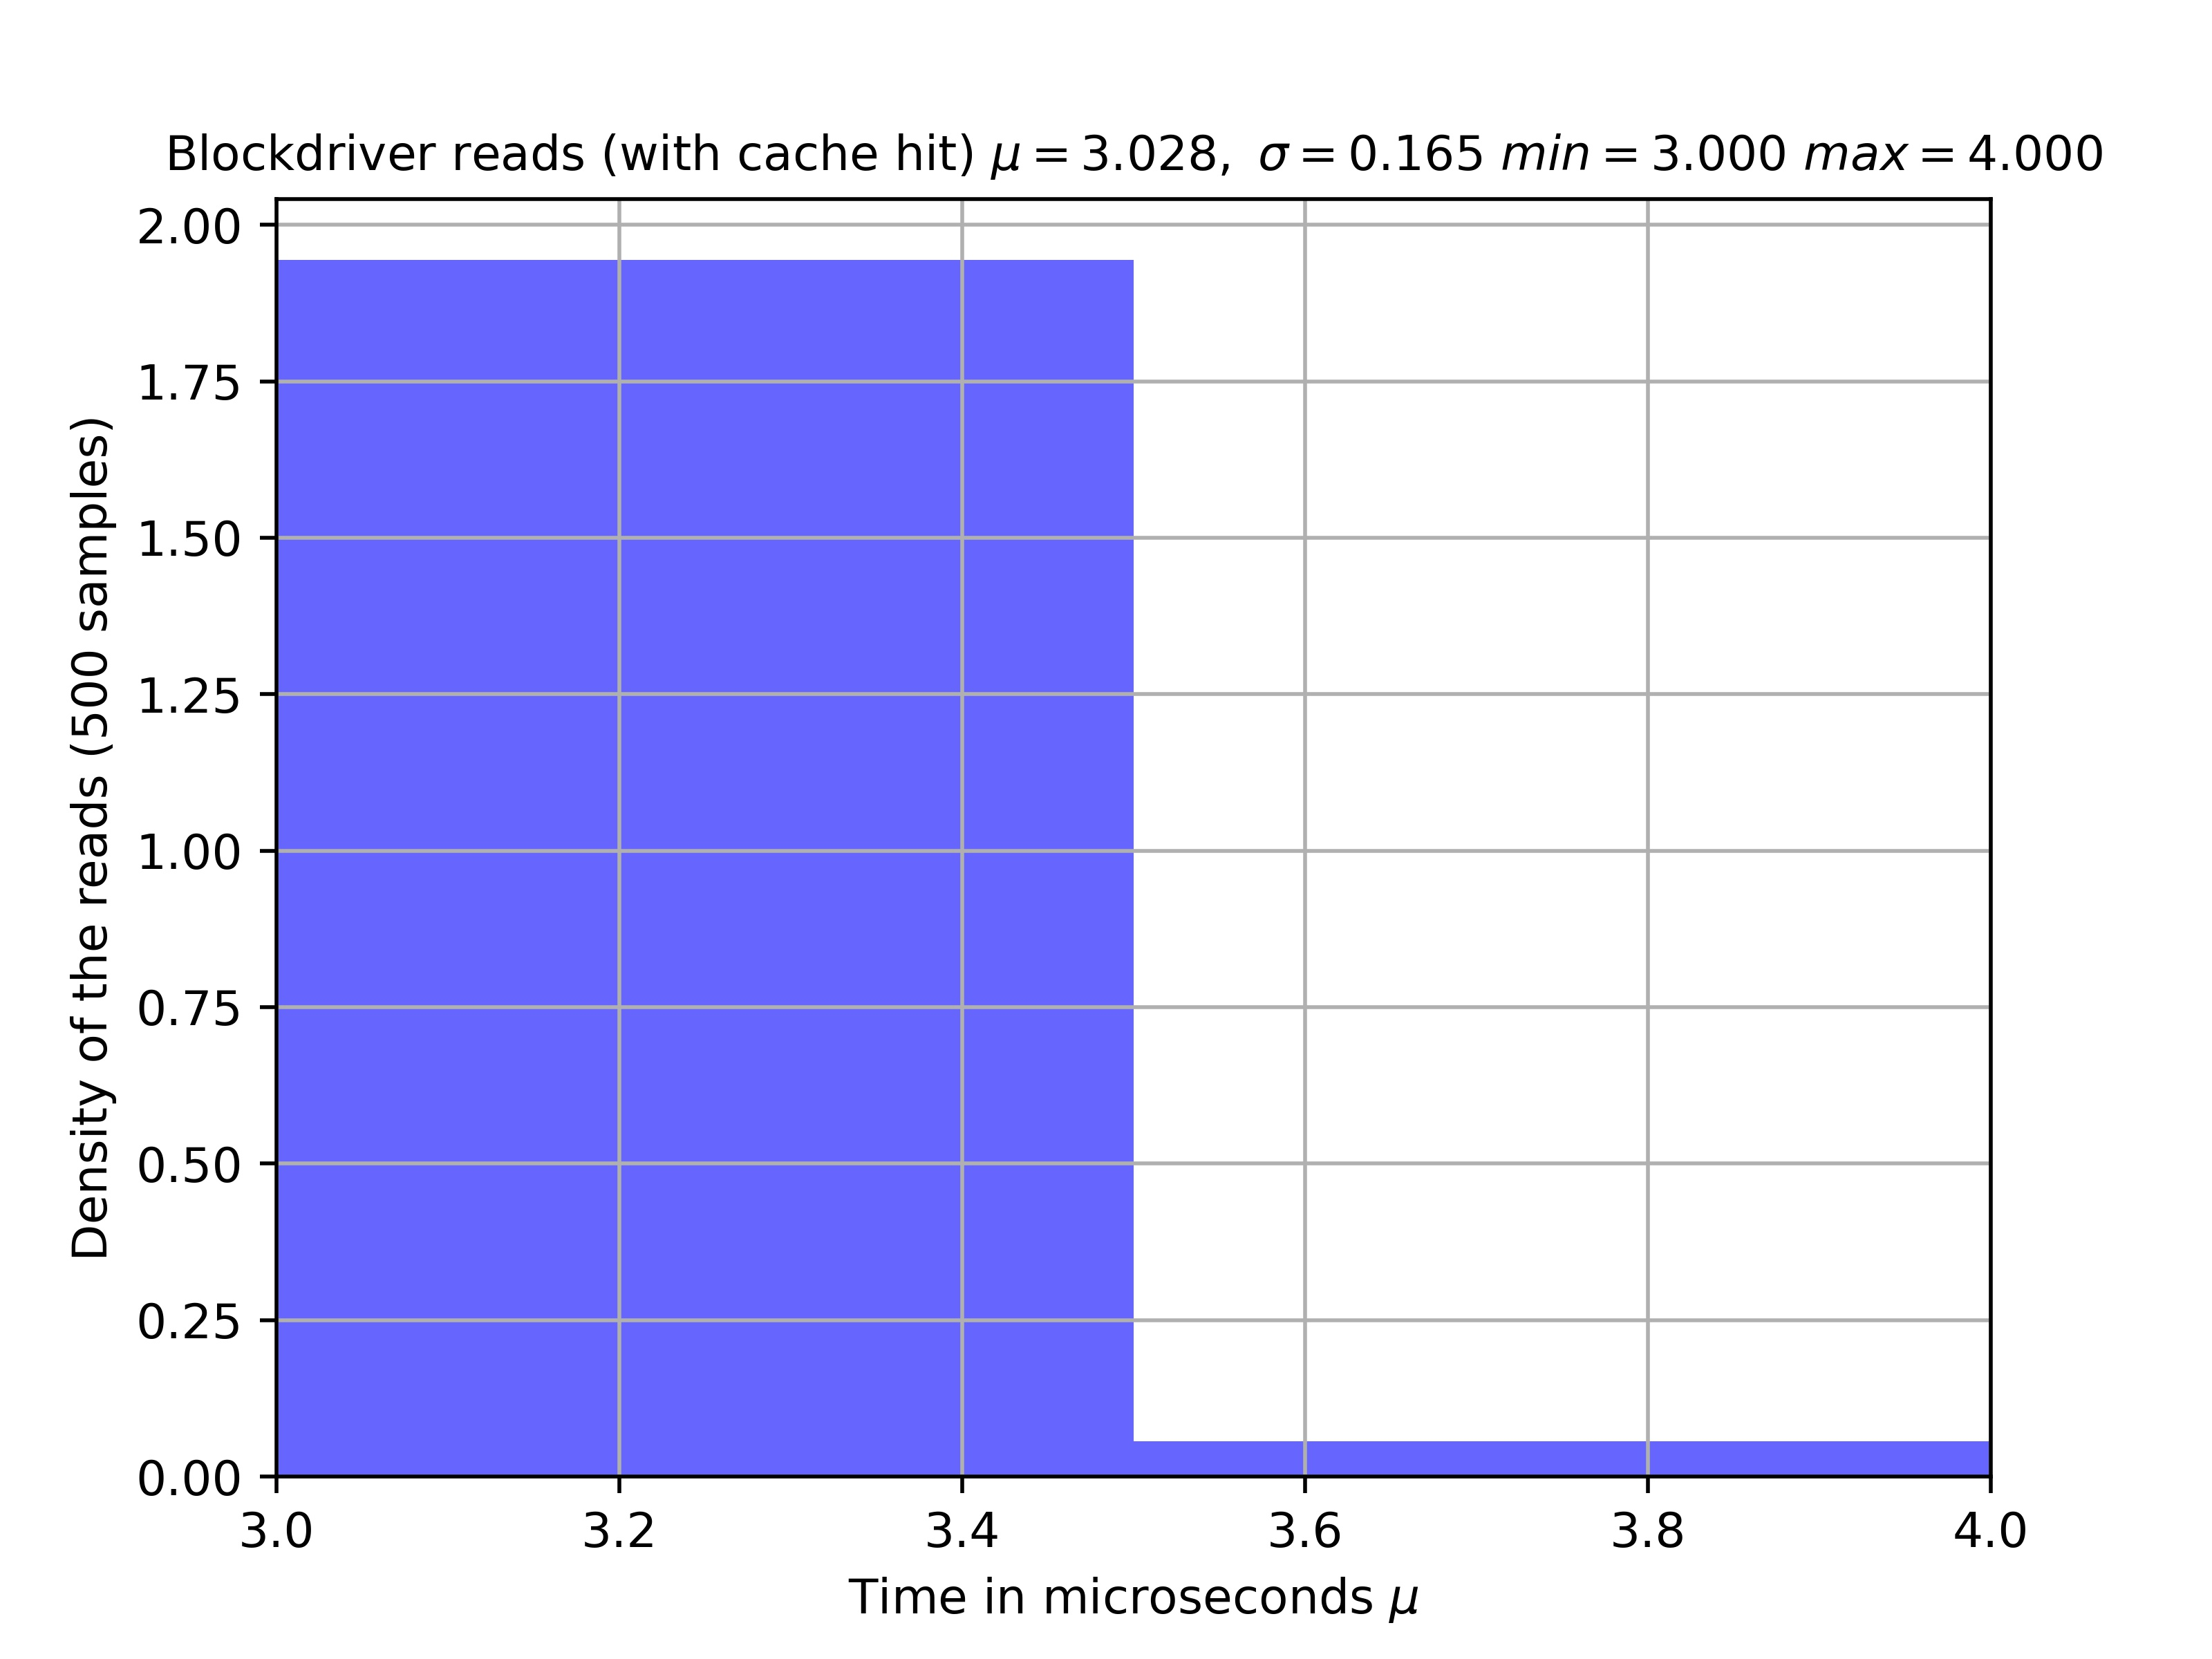
\includegraphics[width=12cm]{images/filesystem/benchmark_read_cache.jpg}
    \caption{Read in the filesystem with cache hit}
    \label{fig:galaxy}
\end{figure}


\section{The Filesystem}

\subsection{What is a filesystem}

In computer science, a \href{https://en.wikipedia.org/wiki/File_system}{\texttt{file system}} is a method of organizing and storing data on a computer's storage devices, such as hard drives, solid-state drives, and USB flash drives. A file system provides a way to organize and access data by creating a \textbf{hierarchical structure} of files and directories.
At its most basic level, a file system provides a way to store and retrieve files on a storage device. However, modern file systems also provide additional functionality, such as file permissions and security features, support for different file types and data compression, and data recovery features.
\begin{itemize}
A file system typically consists of several key components, including:
    \item Data structures: A file system uses various data structures, such as \texttt{directories}, \texttt{files}, and \texttt{blocks}, to organize and store data on a storage device.
    
    \item  File naming conventions: A file system provides a way to name files and directories, typically using a hierarchical structure of names separated by slashes or backslashes. For example, FAT follows the \texttt{8 3 naming convention}.
    
    \item  Data access methods: A file system provides various methods for accessing and manipulating data stored on a storage device, such as reading, writing, and deleting files.
    
    \item Security features: A file system can provide various security features, such as file permissions and encryption, to protect data stored on a storage device. This is out of the score for this assignment.
    
\end{itemize}

\subsection{The fat family and its differences}


\href{https://en.wikipedia.org/wiki/File_Allocation_Table}{\texttt{FAT (File Allocation Table)}} is a file system used on many types of storage media, including floppy disks, USB flash drives, and memory cards. The FAT file system was introduced by Microsoft in 1977 and has since become one of the most widely used file systems due to its simplicity and compatibility with a wide range of operating systems.

\begin{figure}[htp]
    \centering
    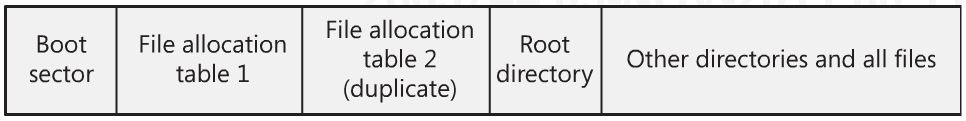
\includegraphics[width=12cm]{images/filesystem/fat_structure.jpg}
    \setcaptioncitation{https://social.technet.microsoft.com/wiki/contents/articles/6771.the-fat-file-system.aspx}
    \caption{Structure of a fat disk}
    \label{fig:galaxy}
\end{figure}


The FAT file system uses a file allocation table to keep track of the location of files and directories on the storage media. This table is essentially a map that lists the clusters (blocks of storage space) that are allocated to each file and directory on the disk.
One of the key features of the FAT file system is its use of \texttt{8.3 filenames}, which are filenames consisting of up to eight characters followed by a three-character extension. This limit on the length of filenames and the use of a limited character set (only uppercase letters, numbers, and a few special characters) was a limitation of early computing hardware but has since become a standard that is still used today. One of the extra milestones was to implement long entries in the filename to overcome this limitation.

\begin{figure}[htp]
    \centering
    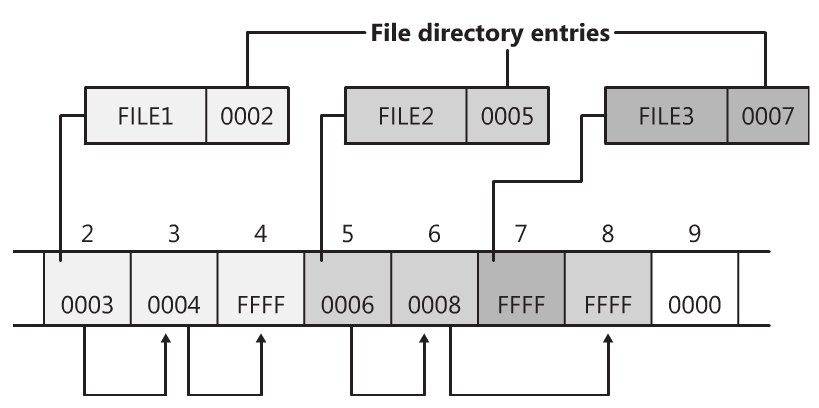
\includegraphics[width=12cm]{images/filesystem/fat_example.png}
    \setcaptioncitation{https://social.technet.microsoft.com/wiki/contents/articles/6771.the-fat-file-system.aspx}
    \caption{Example of a fat table}
    \label{fig:galaxy}
\end{figure}


The \href{https://fr.wikipedia.org/wiki/FAT32}{\texttt{FAT32}} file system is an updated version of the original FAT file system and includes several key differences compared to other FAT filesystems, such as \href{https://fr.wikipedia.org/wiki/FAT12}{\texttt{FAT12}} and \href{https://fr.wikipedia.org/wiki/FAT16}{\texttt{FAT16}}
\begin{itemize}
    \item Maximum partition size: One of the key differences between FAT32 and earlier FAT filesystems is the maximum \texttt{partition size}. FAT12 and FAT16 have limitations on the size of the partition they can support. FAT12 supports partitions up to 16MB, while FAT16 supports up to 2GB. FAT32, on the other hand, supports partitions up to 2 terabytes (TB). 
    \item Cluster size: Another difference between FAT32 and earlier FAT filesystems is the  \texttt{cluster size}. In FAT12 and FAT16, the cluster size is fixed, meaning that the entire partition is divided into clusters of a specific size. However, in FAT32, the cluster size can be adjusted to match the size of the partition. This can help improve the efficiency of the file system by reducing the amount of wasted space on the disk. In the SD card used for the tests, the cluster size was 4096 bytes divided into 8 sectors of 512 bytes.
    \item File and directory size limits: FAT12 and FAT16 have limitations on the maximum size of individual files and directories. FAT12 supports file sizes up to 32MB, while FAT16 supports file sizes up to 2GB. In addition, both FAT12 and FAT16 have limitations on the number of files and directories that can be stored on a partition. FAT32 removes these limitations, allowing for larger files and more files and directories on a single partition.
\end{itemize}
    
In summary, FAT32 offers several key improvements over earlier FAT filesystems, including support for \texttt{larger partitions}, \texttt{larger files and directories}, and \texttt{improved performance}.

\subsection{Understanding the fat32 specification}

Understanding the fat32 specification was a daunting task. I divided this big task into multiple parts:

\begin{itemize}
    \item  Gather some resources about fat32 on the internet. I found multiple websites that helped me to better understand the fat32 specification. 
    \item  Then I tried to get the big picture. How does fat32 work? What are key concepts?
    \item  Looked up unfamiliar terms. What is a cluster? What is a sector? A lot of terms were unknown to me at the beginning, and I had to learn all of them.
    \item Then I broke down each section into smaller, more manageable sections. It helped me to understand fat32 step by step.
    \item I began tackling the helper functions, which proved to be simpler and facilitated a seamless transition into the realm of fat.
    \item In the end, I completed the implementation of the FAT32 functions, starting with the reading functions and concluding with the writing functions.
\end{itemize}

\subsection{The actual implementation}

The implementation of the \texttt{fat32.c} file spans an extensive codebase comprising more than 2000 lines, making it impractical to provide a comprehensive explanation within the confines of this report. However, this section aims to shed light on the key aspects and main lines of the implementation. For a more thorough understanding, interested readers are encouraged to delve into the intricacies by browsing the source code directly.

Despite the complexity of the implementation, it is possible to discern an overarching structure that can be roughly categorized into three distinct sections. These sections delineate fundamental components and crucial operations that collectively form the larger picture of the \texttt{fat32.c} implementation.

While this report may not delve into the intricate details of each line of code, it seeks to provide a high-level overview and highlight the main elements and concepts of the implementation. By exploring these key components, readers can gain a solid grasp of the underlying principles and functionalities driving the \texttt{fat32.c} file.

\subsection{The data structures used in the filesystem}

\subsubsection{fat32\_filesystem}

The fat32 implementation has three distinct data structures that play a crutial role. The first among them is the \texttt{fat32\_filesystem} structure. This particular structure encapsulates crucial details and metadata that are fundamental to the functioning and management of the fat system as a whole. Without this data structure, we wouldn't be able to convert the lba address of a cluster number. By encompassing critical information, the \texttt{fat32\_filesystem} structure forms a foundational component, facilitating the overall organization, operation, and accessibility of data within the fat32 implementation.

\begin{lstlisting}[caption={fat32\_filesystem},captionpos=b,language=C,frame=single,breaklines]
struct fat32_filesystem {
    struct block_driver *b_driver;
    struct fat32_entry root_directory;
    uint32_t cluster_begin_data;
    uint32_t sectors_per_fat;
    uint32_t first_cluster_root_directory;
    uint8_t  sectors_per_cluster;
    uint16_t numbers_sectors_reserved;
    uint8_t  fat32_number;
    uint32_t next_free_cluster_hint;
};
\end{lstlisting}

\subsubsection{fat32\_entry}

The \texttt{fat32\_entry} data structure is specifically designed to work with fat32. It is connected to fat32 in a way that prevents the compiler from optimizing it (using the packed keyword), ensuring its essential role. The purpose of \texttt{fat32\_entry} is to uniquely identify a specific entry, such as a file or folder, within the fat32 system. We can draw an analogy to the primary key in a database.. When a program possesses a value of \texttt{fat32\_entry}, it becomes capable of accessing and reading the corresponding file or folder, regardless of the specific implementation being used. This connection between \texttt{fat32\_entry} and the associated entities enables seamless retrieval and interpretation of data within the fat32 system.

\begin{lstlisting}[caption={fat32\_entry},captionpos=b,language=C,frame=single,breaklines]
struct fat32_entry {
    char name[11];
    uint8_t attribute;
    uint8_t reserved_zero_entry;
    uint8_t creation_time;
    uint8_t empty[6];
    uint16_t cluster_high;
    uint16_t last_modifier_time;
    uint16_t last_modified_date;
    uint16_t cluster_low;
    uint32_t file_size;
} __attribute__((packed));
\end{lstlisting}

\subsubsection{fat32\_handle}

In simple terms, the \texttt{fat32\_handle} is a structure that helps us identify a specific entry, such as a file or directory, and enables us to interact with it. The key distinction between fat32\_entry and \texttt{fat32\_handle} is that the former is in a sense "stateless", meaning it only provides identification information, while the latter stores additional state information alongside it. This stored state allows us to have certain effects or keep track of specific information related to the entry.

For instance, with \texttt{fat32\_handle}, we can maintain the position of a cursor within a file, which is useful for seeking to different parts of the file. It can also help us keep track of the current directory by storing an index, which is beneficial for reading directory contents.

The primary purpose of the \texttt{fat32\_handle} structure is to facilitate communication and interaction with the library built on top of it. By utilizing \texttt{fat32\_handle}, we can effectively perform various operations and access specific functionalities provided by the library. It serves as a helpful tool for managing the state and accessing relevant information associated with a particular entry in the fat32 file system.

\begin{lstlisting}[caption={fat32\_handle},captionpos=b,language=C,frame=single,breaklines]
struct fat32_handle {
    // Current entry
    struct fat32_entry entry;
    // Information about the cluster
    uint32_t current_cluster;
    uint32_t relative_sector_from_cluster;
    // Information for the c library on top of it
    union {
        uint32_t directory_offset;
        uint32_t file_position;
    };
    char *path;
    bool is_directory;
    // Entries about the parent - required to modify entry
    uint32_t parent_cluster_number;
    uint32_t parent_cluster_offset;
};
\end{lstlisting}

\subsection{Functions used to implement the filesystem}

The functions in the implementation can be broadly classified into three main categories.

The first category consists of \textbf{helper functions}. These functions are designed to assist in carrying out more complex routines. They do not produce any side effects or make any modifications to the system. Instead, they provide support and aid in performing specific tasks within the implementation.

The second category comprises functions that are responsible for \textbf{performing operations on the fat32 file system}. These functions directly interact with the file system, executing actions such as reading, writing, or modifying data within the fat32 structure. They play a crucial role in ensuring the proper functioning and manipulation of the file system.

The third and final category encompasses functions that fulfill the specific requirements of the library, allowing it to effectively \textbf{interact with the file system}. These functions are tailored to meet the needs and demands of the library, providing the necessary functionalities and interfaces for seamless communication between the library and the underlying file system.

\subsubsection{Helper functions}

The first part consists of helper functions. These functions don't cause any problems and are used for three important reasons:
\begin{itemize}
    \item Improved readability: When we read the source code of a function, having helper functions makes it easier to understand what the function does. It helps us quickly grasp the purpose and functionality of the code. 

    \item Avoiding duplication: By using helper functions in multiple places, we can avoid repeating the same code over and over again. This saves us time and effort, making the code more efficient and manageable.

    \item Easier testing and bug detection: Helper functions can be tested more easily and independently. This allows us to identify and fix any errors or bugs in the code more quickly. By isolating specific functionalities in helper functions, we can focus on testing them individually and ensure their reliability. It enables us to employ unit tests as well.

    \item Overall, employing helper functions simplifies the code, promotes code reuse, and enhances the efficiency of testing and bug detection processes.
\end{itemize}

\begin{lstlisting}[caption={Example of unit test (true or false indicates if the name is for a directory)},captionpos=b,language=C,frame=single,breaklines]
void _test_name_valid(void) {
    // Test filenames - examples from here (http://elm-chan.org/docs/fat_e.html)
    assert(is_fat32_name_valid("FILENAME.TXT", false));
    assert(!is_fat32_name_valid("FILENAME.TXT", true));
    assert(is_fat32_name_valid("file.txt", false));
    assert(!is_fat32_name_valid("file.txt", true));
    assert(is_fat32_name_valid("NOEXT", true));
    assert(!is_fat32_name_valid(".cnf", true));
    assert(!is_fat32_name_valid(".cnf", false));
    assert(!is_fat32_name_valid("new file.txt", false));
    assert(!is_fat32_name_valid("new file.txt", true));
    assert(!is_fat32_name_valid("file[1].2+2", false));
    assert(!is_fat32_name_valid("two.dots.txt", false));
    assert(!is_fat32_name_valid("two.dots", true));
    return;
}
\end{lstlisting}


\subsubsection{Functions that perform operations on the fat32 filesystem}

The second category of functions includes those that perform specific operations within the fat32 system, but are not directly related to user actions like opening files, reading, or creating directories. These functions handle internal tasks that are essential for the proper functioning of the fat32 system.

For example, one function in this category is \texttt{get\_next\_cluster}. This function is responsible for reading the content of the next cluster when provided with a cluster number. Another function, \texttt{fat32\_remove\_chain}, is another example. It is designed to delete an entire chain of clusters and update the system's state by writing changes to the disk.

Among all the functions in this category, two hold particular significance. They are used in multiple other functions and play a critical role in the fat32 system. These functions require special attention and scrutiny because if they contain any bugs or errors, the entire file system may quickly become unstable. This could result in the violation of important invariants required by the fat32 system, rendering it in an undefined or an inconsistent state.

\subsubsection{fat32\_resolve}

When we talk about resolving a path in the fat32 filesystem, it means finding the exact location or full path of a file or directory based on the given path. A path is like a set of directions that tells us where a file or directory is in relation to the main or root directory of the filesystem.

The function \texttt{fat32\_resolve} is responsible for this task. It takes a path as input and returns a handle, which is like a reference or pointer, to the file or directory that matches the given path. However, if the input path is not valid or doesn't exist, \texttt{fat32\_resolve} will give an error instead of a handle.

To understand how \texttt{fat32\_resolve} works, we can look at its pseudo code. This pseudo code is a simplified version of the actual code that explains the steps and logic used in the function to resolve the path and find the corresponding file or directory.

\begin{algorithm}
\caption{Resolve path}
\begin{algorithmic}
\Procedure{fat32\_resolve\_path}{$\text{path}, \text{handle}$}
    \State \Call{assert}{path\_is\_absolute}
    
    \While{not \Call{is\_path\_end}{}()}
            \State $\text{current\_path}, \text{next\_path} \gets \text{split\_path}()$
            
            \State $\text{not\_found} \gets \Call{find\_directory}{\text{current\_path}}$
            \If{$\text{not\_found}$}
                \Return $\text{FS\_ERR\_NOTFOUND}$
            \EndIf
            \If{\Call{is\_file}{$\text{current\_path}$} \textbf{and} \Call{is\_not\_last}{}()}
                \State \Return $\text{FS\_ERR\_NOTDIR}$
            \EndIf
            
            \State $\text{path} \gets \text{next\_path}$
    \EndWhile

    \State \Call{fill\_handle}{handle}
\EndProcedure
\end{algorithmic}
\end{algorithm}

\subsubsection{fat32\_find\_directory}

The second essential function is designed to \texttt{traverse} through a directory's files and perform a specific function or operation on it. It essentially goes through each entry, one by one, and executes the provided function for each entry. This function operates as a loop, ensuring that the desired operation is carried out on all the folders within the directory.

To understand the inner workings of this function, we can refer to its pseudo code. This code provides a simplified explanation of the steps and logic involved in executing the function and performing the desired operation.

In summary, the first function helps us navigate paths, while the second function allows us to \texttt{iterate} through a directory's entries and perform a specified operation on each entry.

\begin{algorithm}
\caption{fat32\_find\_directory}
\begin{algorithmic}[1]
\Procedure{fat32\_find\_directory}{path, directory\_entry}
    \State $next \gets \text{true}$
    \State $current\_cluster\_number \gets \text{get\_cluster\_number}()$
    \State $lba\_start \gets \text{get\_lba\_from\_cluster}(current\_cluster\_number)$

    \While{$next$}
        \For{$j \gets 0$ to $sectors\_per\_cluster$}
            \State $\text{read\_block}(lba, data)$

            \For{$i \gets 0$ to $number\_directories\_per\_block$}
                \State $current\_entry \gets data[i]$

                \If{$\text{compare\_filename\_with\_entry}(current\_entry, path)$}
                    \State $directory\_entry \gets current\_entry$
                    \State \textbf{return}
                \EndIf

                \If{$current\_entry.\text{name}[0] == END\_DIRECTORY$}
                    \State \textbf{return} $FS\_ERR\_NOTFOUND$
                \EndIf
            \EndFor
        \EndFor

        \If{$lba\_start == cluster\_begin\_data$}
            \State $next \gets 0$
            \State \textbf{continue}
        \EndIf

        \State $\text{fat32\_get\_next\_cluster}(current\_cluster\_number, next\_cluster\_number)$

        \If{$next\_cluster\_number \geq END\_CLUSTER$}
            \State $next \gets 0$
        \EndIf
    \EndWhile
\EndProcedure
\end{algorithmic}
\end{algorithm}

 \subsubsection{Final words}

As a programmer, I want to emphasize that all functions are important, and I haven't overlooked the significance of the other functions. However, let's add a touch of humor to this section of the report. Imagine if the incredible team at AOS gives a magical oracle that could instantly generate a ready-to-use code with exactly two perfectly correct functions. We are allowed to get two functions. In that imaginary scenario, these two functions would undeniably be the two I would ask by writing to the staff.

\subsubsection{The last category}

The final group of functions includes those that perform specific operations on the fat32 and will act similar to an \texttt{entry point}. These functions are designed to carry out various \texttt{tasks} within the fat32 system.

The table below provides an explanation of what each function does, outlining their respective functionalities. These functions are accessed through RPC using the \texttt{aos\_rpc} framework and the library implemented in fopen.

In simpler terms, these functions are like tools that can be used as \texttt{entry point} by other processes to interact with and perform operations on the fat32 system. They offer a range of functionalities that can be accessed remotely through a library, making it easier for different processes to manipulate the fat32 system.

\begin{lstlisting}[caption={"Entry points" in the filesystem},captionpos=b,language=C,frame=single,breaklines]
errval_t fat32_open(struct fat32_filesystem *fs, const char *path, struct fat32_handle **handle);
errval_t fat32_close(struct fat32_filesystem *fs, struct fat32_handle *handle);
errval_t fat32_stat(struct fat32_filesystem *fs, const struct fat32_handle *handle, struct fs_fileinfo *info);
errval_t fat32_read(struct fat32_filesystem *fs, struct fat32_handle *handle, void *data, size_t size, size_t *nb_bytes_read);
errval_t fat32_write(struct fat32_filesystem *fs, struct fat32_handle *handle, const void *data, size_t size, size_t *nb_bytes_written);
errval_t fat32_seek(struct fat32_filesystem *fs, struct fat32_handle *handle,enum fs_seekpos whence,off_t offset);
errval_t fat32_tell(struct fat32_filesystem *fs, struct fat32_handle *handle, size_t *pos);
errval_t fat32_open_directory(struct fat32_filesystem *fs, const char *path, struct fat32_handle **handle);
errval_t fat32_close_directory(struct fat32_filesystem *fs, struct fat32_handle *handle);
errval_t fat32_read_next_directory(struct fat32_filesystem *fs, struct fat32_handle *handle, char **new_name);

errval_t fat32_remove(struct fat32_filesystem *fs, const char *path);
errval_t fat32_remove_directory(struct fat32_filesystem *fs, const char *path);
errval_t fat32_create(struct fat32_filesystem *fs, const char *path, struct fat32_handle **handle);
errval_t fat32_mkdir(struct fat32_filesystem *fs, const char *path, struct fat32_handle **handle);
\end{lstlisting}

\subsubsection{Concurency inside the filesystem}

In a real-world operating system, multiple users can \texttt{simultaneously} write to a file. This necessitates the capability to handle \textbf{concurrent requests} to the file system without compromising its integrity. To address this, the implemented solution utilizes a large lock encompassing the entire file system. When a function is invoked from the \texttt{aos\_rpc} framework, it is locked by this mechanism. Alternatively, a read-write lock can be employed, as interleaved multiple reads pose no problems. However, the main concern lies with the write operations, for which locking is crucial. This approach mirrors the principles employed in other concurrent algorithms. 

\subsubsection{Do we really need lock in our case? - analogy with golang channels}

\href{https://go.dev/}{Go (Golang)}   is a programming language developed by Google. It focuses on simplicity, efficiency, and concurrency. It features a garbage collector, built-in concurrency primitives, and is widely used for web development, systems programming, and networking applications.

In \href{https://go.dev/}{\texttt{Go (Golang)}, \href{https://www.educative.io/answers/what-is-a-goroutine}{\texttt{a goroutine}} is a lightweight concurrent execution unit. It is a function or method that can be launched independently and run concurrently with other goroutines within the same program. Goroutines are managed by the Go runtime and utilize a small amount of memory, allowing for the creation of thousands or even millions of goroutines. They are designed to efficiently handle concurrent tasks, enabling concurrent programming without the overhead of traditional threads. Goroutines communicate with each other using channels, which provide synchronized and safe communication between concurrent goroutines. The combination of goroutines and channels forms the foundation of Go's powerful concurrency model.

In Go (Golang), \href{https://www.educative.io/answers/what-are-channels-in-golang }{\texttt{channels}} are a fundamental feature used for communication and \texttt{synchronization} between goroutines. A channel is a typed conduit that allows for the sending and receiving of values between concurrent goroutines. It provides a safe and efficient way to exchange data and coordinate actions among goroutines.

In Golang, there are essentially two main techniques to lock a critical section within a code snippet. The first approach involves using a traditional mutex, similar to other programming languages. However, Golang offers a remarkably elegant solution (in my honest opinion) using channels. In this method, all goroutines (referred to as threads in Golang jargon) send their requests through a channel. Subsequently, another goroutine situated at the channel's endpoint processes the received requests sequentially, ensuring that the actions are executed \textbf{in a sequential order and avoiding any interleaving of two critical sections}.

Now comes a fundamental question: Is it really necessary to have a \textt{lock} in our function? Upon closer examination, I fail to identify any scenario where two requests to the initialization process could execute code in an interleaved manner. Why is this the case? Well, all calls to the filesystem within the function are \textbf{blocking} and operate on a \textbf{completion basis}. This means that we only exit the \texttt{critical section} in two situations: when the call is completed successfully or when an error occurs. In both cases, the execution of the function concludes, allowing the next request to enter the \texttt{critical section}. Consequently, we encounter \textbf{no interleaving}. It is important to note that the filesystem and block driver are exclusively present in the init process. While discussing Golang within this report may seem surprising, upon reflection, we can indeed see that the concurrency pattern we are encountering aligns precisely with goroutines and channels in Golang.

Let's approach this question from a critical standpoint. Does having a lock-free filesystem imply that I am the next superstar PhD student in systems? Absolutely not. If the current operating system we have developed were to adopt such an \texttt{architecture}, we would consider the design to be mediocre (in a real world setup). The only reason I can consider avoiding locks in this particular case is due to two specific properties. Firstly, the filesystem (which is the sole component we need to trust in order to maintain FAT32 invariants) resides in the init process. Secondly, all calls to this component are blocking and execute upon completion. It is these two properties that enable me to eliminate the need for locks in this context. In scenarios where the block driver is in a waiting state, incorporating a non-blocking call would enable another process to execute computations during the waiting period. However, adopting this approach would necessitate the implementation of a file system lock to ensure proper synchronization and prevent data integrity issues. 
\subsection{Communication with the read world}

We now have a fully functional file system that allows us to perform various operations like reading, writing, adding and deleting directories. However, it would be unwise to assume that our work is complete.

Initially, our file system is only accessible to the init process and is not visible to the rest of the operating system. To make the most of its functionality, we need to establish a gateway for our file system. The question arises: How should we integrate the file system? Should it be as a library that other processes can utilize? Should we use RPC calls and centralize everything within the init process?

\subsubsection{A full barrelfish library}

The first idea is quite creative. It suggests having a basic service, called the block driver, residing in the init process. Any application that wants to work with the fat32 formatted disk could include a specific file, like "fat32.h," and directly call functions to manipulate the disk using a pointer to the block driver. To ensure safe communication between multiple processes, the critical part of the block driver would be protected by a lock.

Although this idea remains at the conceptual stage and may seem eccentric and challenging to implement, it serves the purpose of exploring different operations and ideas. Without the exposure to Barrelfish and this course, I would have likely stuck to more conventional Unix-based approaches and not considered such unconventional ideas.

Taking time to ponder this idea, I see potential benefits. In an operating system like \href{https://barrelfish.org/}{\texttt{Barrelfish}}, which is a \href{https://en.wikipedia.org/wiki/Microkernel}{\texttt{microkernel}} offering flexibility and unique behaviors compared to \href{https://en.wikipedia.org/wiki/Monolithic_kernel}{\texttt{monolithic kernels}} like Linux, there are advantages to be found. For instance, imagine an application with heavy input/output (I/O) demands. By directly interacting with the block driver, each call can \texttt{bypass} the \texttt{overhead} of RPC calls, saving valuable time and system resources. Another advantage is that the file system is implemented as a \texttt{library}. Skilled programmers could \texttt{customize} and optimize this library for specific application patterns, enhancing performance for specific tasks.

In conclusion, this eccentric idea showcases how a system like \texttt{Barrelfish} fosters the imagination of diverse computer systems. By moving a significant portion of the kernel into \texttt{userspace}, it provides additional flexibility and opens up possibilities for innovative approaches.


\subsubsection{A single service that lies in the init process}

The second idea and solution involve integrating the filesystem directly into the init process alongside the block driver. Any process that wants to interact with the filesystem will simply use a \texttt{high-level API} to make RPC calls for their requests. This design decision is less unique compared to the first idea and resembles the structure found in \href{https://fr.wikipedia.org/wiki/Unix}{\texttt{UNIX-like systems}}.

There are a few reasons why I chose this approach. Firstly, it aligns with the overall consistency of our system, which is important for simplifying our RPC infrastructure. Since all services are contained within the init process, this design decision maintains consistency within our team. However, it does have its drawbacks and disadvantages, and whether it is the right choice remains uncertain. Nonetheless, since we decided on this direction, it makes sense for me to follow the same approach for my individual milestone.

Another factor to consider is the available time. Building and integrating a fat32 file system is a complex software engineering project, not just a simple coding exercise. Like any other project, time constraints must be taken into account. Choosing a more standard design provides assurance that the project will yield results and have fewer surprises compared to a more creative implementation.

Therefore, I implemented all the necessary parts in the \texttt{fat32.c} file to enable interaction with the block driver and perform operations within the filesystem. The filesystem includes a pointer to an instance of the block driver, which allows it to read and write blocks on the disk.

\subsubsection{The "C" Api}

The "C" API in \texttt{fopen.c} is a collection of functions and data structures that allow the shell and other processes to interact with the fat32 file system in a \texttt{standardized} way. It provides a clear and defined interface for communication. This standardized interface ensures that multiple processes can access files and directories simultaneously, enabling them to read from and write to the file system.

The filesystem API includes various functions for different operations. For example, there are functions for creating, opening, reading, writing, and closing files. Additionally, there are functions specifically designed for working with directories, such as creating new directories, listing directory contents, and retrieving file attributes.

By using the filesystem API in userspace, processes can perform a wide range of tasks related to working with files and directories. This includes tasks like copying files, creating new directories, and viewing the contents of a directory. The API provides a consistent and reliable way for processes to interact with the fat32 file system, making it easier to manage and manipulate files and directories in a standardized manner.

The "C" API serves as a wrapper that adds additional functionality and acts as a bridge between a \texttt{Barrelfish} process and the \texttt{aos\_rpc} framework. This API facilitates the communication between the process and the filesystem by sending RPC calls through our \texttt{aos\_rpc} framework.

\begin{lstlisting}[caption={Function filled in libopen},captionpos=b,language=C,frame=single,breaklines]
static int fs_libc_open(char *path, int flags);
static int fs_libc_read(int fd, void *buf, size_t len);
static int fs_libc_write(int fd, void *buf, size_t len);
static int fs_libc_close(int fd);
static off_t fs_libc_lseek(int fd, off_t offset, int whence);

static errval_t fs_mkdir(const char *path);
static errval_t fs_rmdir(const char *path);
static errval_t fs_rm(const char *path);
static errval_t fs_opendir(const char *path, fs_dirhandle_t *h);
static errval_t fs_readdir(fs_dirhandle_t h, char **name);
static errval_t fs_closedir(fs_dirhandle_t h);
static errval_t fs_fstat(fs_dirhandle_t h, struct fs_fileinfo *b);
\end{lstlisting}

\subsubsection{Benchmarking the filesystem}

Benchmarking the filesystem lacks a singular definitive approach due to the presence of numerous viable methods to evaluate its performance. Consequently, during the benchmarking process, three distinct decisions were made to ensure a clear and rigorous evaluation of the filesystem's performance.

The initial decision made during the benchmarking process involves opting not to test the filesystem exclusively from the fopen functions but instead directly evaluating the \texttt{fat32.c} file itself. This choice is driven by the consideration of \texttt{dependencies} and their potential impact on the observed performance. To illustrate this, let's consider two scenarios.

In the first scenario, let's assume we have an exceptionally fast implementation of an RPC call. If we were to benchmark the filesystem solely based on the \texttt{fopen.c} functions, the overall filesystem performance would appear faster due to the swift execution of the RPC call. However, this may not accurately reflect the \texttt{true performance} of the filesystem as a whole.

It is essential to recognize that the RPC handler is an \texttt{external component} that is \texttt{extrinsic} to the filesystem. Thus, any fluctuations in its speed can distort the perception of the filesystem's performance. By testing directly from the \texttt{fat32.c} file and bypassing the specific dependency of the RPC handler, we aim to obtain a more \texttt{accurate} evaluation of the filesystem's performance, unadulterated by the potential confounding effects of external components.

The second decision made in the benchmarking process pertains to the evaluation of \texttt{peak performance} concerning the actual number of \texttt{bytes read} and \texttt{written} to the disk \texttt{per second}. This particular assessment falls under the purview of benchmarking the block driver, not the filesystem itself. It is important to note that the end user's primary concern does not lie in the speed of writing data in terms of bytes per second. In fact, what truly matters in the testing of the filesystem is the speed in cycles required to read from and write to a file.

To illustrate this concept, let's consider a scenario where we have an exceptionally fast block driver, assuming it is ten times faster for the sake of simplicity. Additionally, let's assume that the underlying fat implementation, on average, needs to read ten blocks to access a file of size X. Now, contrast this with a normal block driver that is ten times slower than the aforementioned faster version. In this case, however, the fat implementation only needs to read one block, on average, to access the same file of size X.

In the first scenario with the faster block driver, the overall bandwidth appears more aggressive due to its heightened performance capabilities. However, from the user's perspective, there is no noticeable difference in speed. The perceived speed experienced by the user remains the same in both situations, regardless of the variation in the underlying block driver's performance.

The last decision worth mentioning is that we conduct filesystem testing when there are only a few entries on the disk. This is important because when we write to a new file, it may take longer if we need to locate a new cluster, for instance. In the worst-case scenario, we would have to iterate through the entire FAT32 table entry, which can be a time-consuming process. On the other hand, in a more optimistic scenario, we can find a free entry within the same block if we need to extend the file's size, resulting in a faster operation. It's worth noting that these measurements were performed on a \texttt{freshly formatted filesystem}.

To conclude, \textbf{benchmarking the block driver} primarily revolves around evaluating the \textbf{"true" speed}, which encompasses the actual number of bytes written to the disk per second. On the other hand, \textbf{benchmarking the filesystem} focuses on assessing the \textbf{perceived speed minus the RPC overhead} experienced by the user, which considers the speed in cycles required for reading from and writing to files. We get a max read bandwith around \texttt{1350 bytes per second} without caching and around \texttt{100 gigabytes per second} with caching and perfect temporal locality. The writes are a bit slower. We manage to reach \texttt{900 bytes per second without caching} and \texttt{1350 bytes per second with caching}.



\begin{figure}[htp]
    \centering
    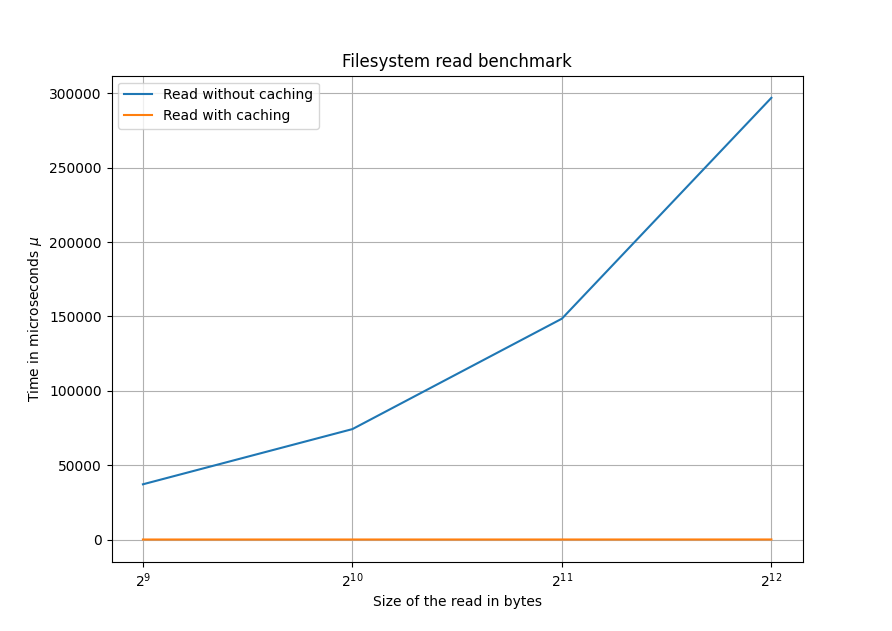
\includegraphics[width=12cm]{images/filesystem/filesystem_benchmark_read.png}
    \caption{Benchmark filesystem read}
    \label{fig:galaxy}
\end{figure}


\begin{figure}[htp]
    \centering
    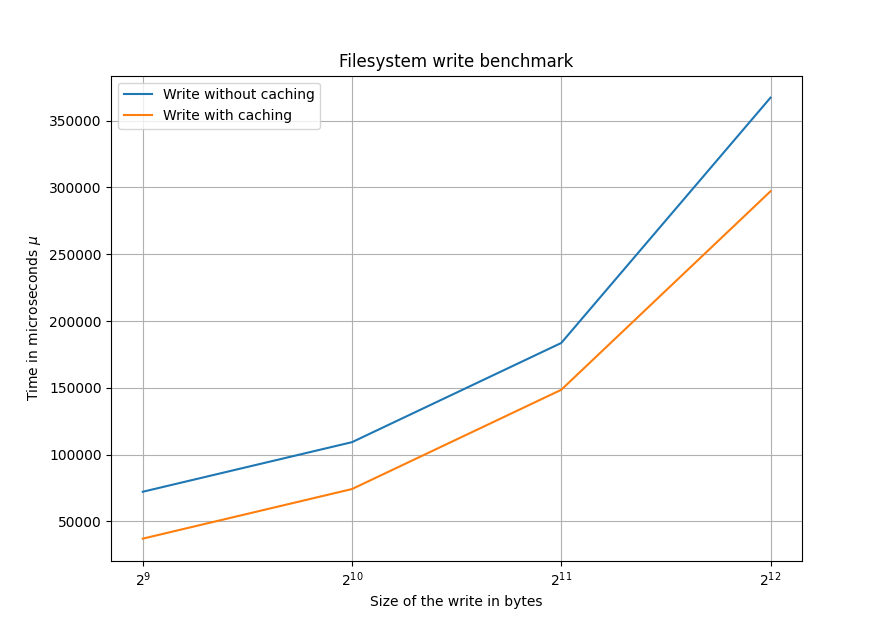
\includegraphics[width=12cm]{images/filesystem/filesystem_benchmark_write.png}
    \caption{Benchmark filesystem write}
    \label{fig:galaxy}
\end{figure}

We can also import elf entries from the computer's file system. ELF files are binary files similar to others, so it makes sense that we can import them from the file system. However, because our block driver is not very fast, importing an elf binary takes some time. It usually takes about one minute for a simple program to import. Here's how the importing process works:

In the process manager, we first check if the name of the binary starts with "/sdcard/". If it does, we import it from the file system using that specific location. Otherwise, we import it from the multiboot options as usual. The process loader module \textfff{dynamically} handles requests to load binary data.

\begin{lstlisting}[caption={Routing the load request to the correct source},captionpos=b,language=C,frame=single,breaklines]
static errval_t _load_elf_internal(const char *path, struct elfimg *img, int *argc, char ***argv) {
    if((strnlen(path, 7) >= 7 && strncasecmp("/SDCARD/", path,7) == 0)) {
        return spawn_load_filesystem(path, img, argc, argv);
    } else {
        return spawn_load_elf(bi, path, img, argc, argv);
    }
}
\end{lstlisting}

\subsubsection{Last but not least, the integration with the shell}

Upon completion of the block driver, a crucial component of our operating system is now \texttt{operational}. However, it is important to note that this achievement does not mark the end of our journey. There remains an open question regarding how we seamlessly \texttt{integrate} this component into \texttt{the broader system}, particularly in terms of \texttt{communication} with the shell.

The integration of the filesystem itself did not pose a significant challenge. Fortunately, the file \texttt{fopen.c} served as a suitable interface, bridging the gap between the shell and the filesystem. By combining these two entities, we were able to establish a connection that allowed for the smooth functioning of the filesystem. Although minor issues surfaced during this integration process, overall, the filesystem performed admirably.

The integration of the filesystem within the shell environment provided us with an opportunity to thoroughly test and expand upon some of the shell's built-in functionalities, such as \texttt{ls} or \texttt{cat} This collaborative environment enabled us to uncover additional issues within the filesystem and address them accordingly. It served as a fertile ground for identifying any potential shortcomings and further refining the filesystem's overall functionality.

\begin{figure}[htp]
    \centering
    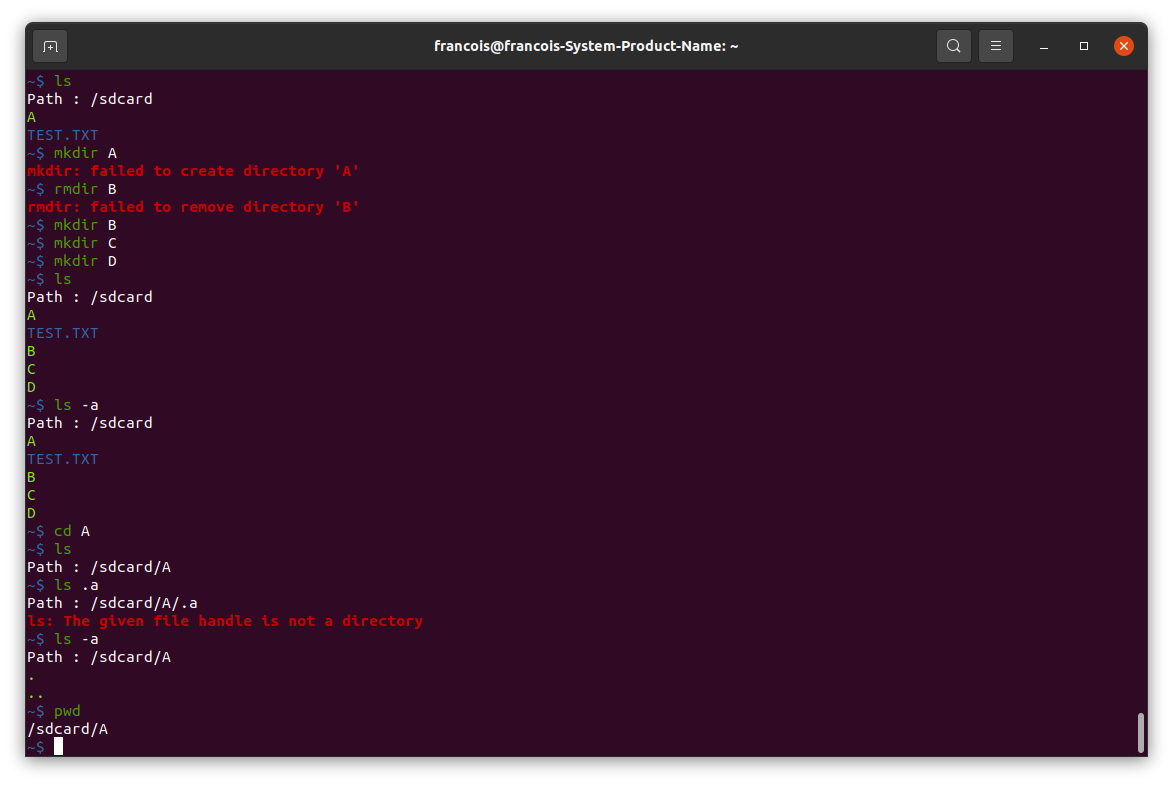
\includegraphics[width=12cm]{images/filesystem/interaction_with_shell.png}
    \caption{Interaction with the shell}
    \label{fig:galaxy}
\end{figure}


\begin{figure}[htp]
    \centering
    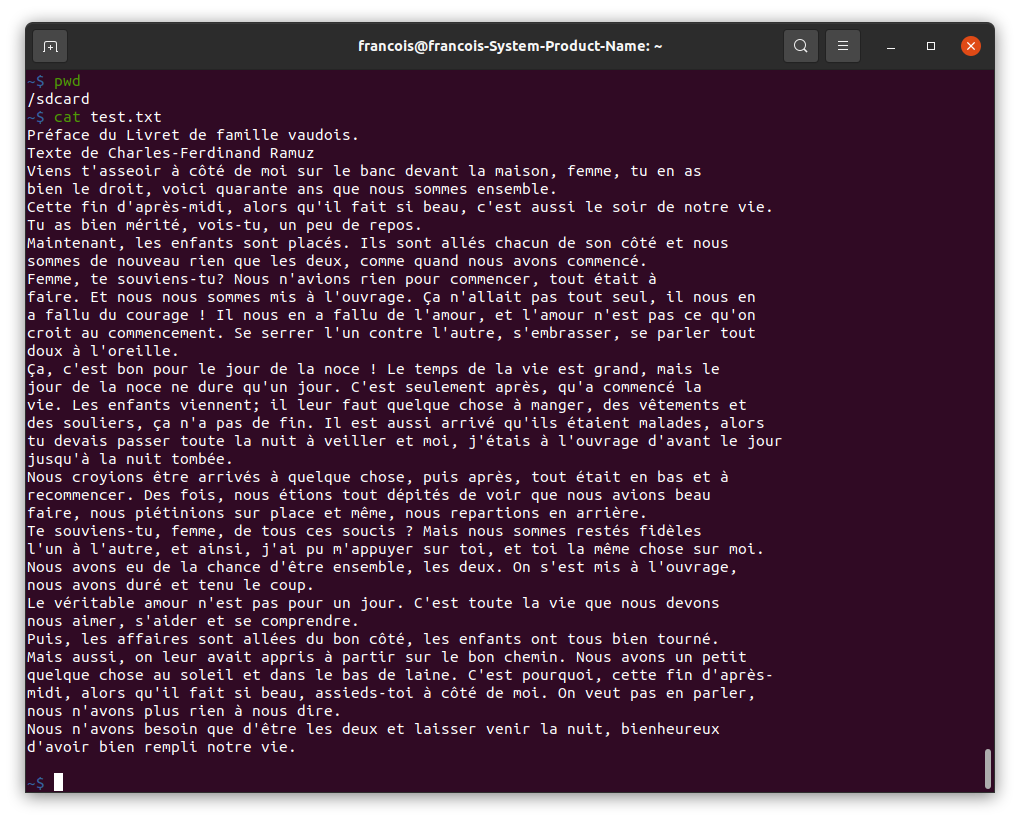
\includegraphics[width=12cm]{images/filesystem/example_cat.png}
    \caption{Cat}
    \label{fig:galaxy}
\end{figure}


\section{Conclusion and next steps}

\subsection{Limitations of our filesystem}

Presently, our filesystem exhibits certain limitations. Listed below are the limitations that we should consider.

\begin{itemize}
    \item The maximum allowed character limit for paths, including the mounting point, is 512 characters.

    \item Our current system lacks support for long filename entries, and we are constrained to adhere to the 8.3 FAT naming convention.

    \item When a directory containing files is deleted, it results in a leak in the FAT table. To mitigate this issue, we can enforce a restriction where users are only allowed to remove empty directories.

    \item Our system currently does not provide support for any timestamps.
\end{itemize}


\subsection{Possible improvements}

Creating a fat32 filesystem was a \texttt{challenging task} that took me longer than expected. I had to write, rewrite, and test over \texttt{2800 lines of code} to reach an acceptable version.

Although the filesystem is functional, there are still areas that can be improved. Here are some potential next steps:

\begin{itemize}
    \item \textbf{Enhance the block driver}: The current block driver is not very fast, and there are several areas where it can be improved. For instance, we can optimize it by reading multiple sectors at once or increasing the device's speed.

    \item \textbf{Develop a more robust test framework}: It would be beneficial to have a simulated disk in the test framework. This way, we can perform operations on the simulated disk and verify if the required fat32 invariants are maintained.

    \item \textbf{Improve file metadata support}: Currently, some important file metadata information is missing. For example, we don't have information about when a file was created. Enhancing the filesystem to include better file metadata support would be beneficial.

    \item \textbf{Refine the code}: Given the time limitations, adhering to the best software engineering practices consistently proved challenging. Consequently, there is significant room for refactoring and improvement.

    \item \textbf{Support for long file name entries}: At present, our filesystem encounters two significant restrictions. Firstly, the path size must not exceed 512 characters. Additionally, we solely accommodate the 8.3 naming convention.
    
\end{itemize}


By addressing these areas of improvement, we can enhance the performance, reliability, and overall quality of the fat32 filesystem implementation.

\subsubsection{Enhance the block driver}

The block device driver we recieved is basic and slow but we can improve it. We can try different approaches to improve performance, such as reading or writing multiple blocks together, using interrupts instead of polling for data transfer, or adjusting the card's clock frequency through the host controller. 

There are still numerous opportunities for improvements within the block driver. One significant advancement would involve negotiating the optimal parameters with the hardware, aiming to achieve the most efficient and effective performance. Additionally, an enhancement worth considering is the implementation of a mechanism that allows for writing multiple blocks simultaneously. By leveraging this approach, we can further optimize data transfer and throughput, potentially enhancing the overall efficiency of the block driver.

\subsubsection{Develop a more robust test framework}

One potential approach we could take to enhance the testing of the \texttt{fat32\_filesystem} is by implementing a mock block driver. By doing so, we would create a simulated environment that emulates the behavior of the actual block driver. This would provide us with a valuable means of conducting unit testing for the \texttt{fat32\_filesystem}, allowing us to thoroughly evaluate its functionality and performance.

\subsubsection{Add metadata in the filesystem}

These entries are currently not included in my filesystem and implementation, but we could add them to the metadata of the files and directories in the FAT32 filesystem.

\begin{itemize}
    \item \textbf{Creation Date and Time}: This records the specific date and time when the file or directory was originally created.

    \item \textbf{Last Modified Date and Time}: This indicates the date and time when the file or directory was last modified or changed.

    \item \textbf{Access Date}: This denotes the date when the file or directory was last accessed or opened.
    
    \item \textbf{Permissions}: These define the access permissions for the file or directory, specifying who can read, write, or execute it.
\end{itemize}

\subsubsection{Improving the quality of the code}

Here are some ideas we can use to improve the quality of the code

\begin{itemize}
    \item \textbf{Modularize the code}: Break down the code into smaller, reusable modules or functions. This improves readability, maintainability, and allows for better code organization.

    \item \textbf{Use meaningful variable and function names}: Ensure that variable and function names accurately describe their purpose and functionality. This improves code comprehension and makes it easier to understand and work with the code.

    \item \textbf{Improve error handling}: Add more error-handling mechanisms throughout the code to handle exceptional scenarios gracefully. This includes handling file system errors, memory allocation failures, and input validation. Even if the code has some primitives for it, we could clearly extend it and make it better. We have no custom errors specific to our implementation.

    \item \textbf{Optimize performance}: Identify potential bottlenecks or areas where the code can be optimized for better performance. This could involve doing disk I/O operations, reducing unnecessary computations, and trying to find better data structures. Optimizing the search for a free cluster is a potential area for improvement.

    \item \textbf{Incorporate design patterns}: Study and apply relevant design patterns to enhance the overall architecture and structure of the filesystem code. Design patterns provide proven solutions to common software design problems and can improve code maintainability and extensibility.
\end{itemize}


\subsubsection{Support for long file name entries}

Currently, within our filesystem, we face two noteworthy limitations that impose certain constraints. Firstly, it is imperative to ensure that the size of the path does not surpass the threshold of \texttt{512 characters}. This restriction is in place to maintain the integrity and efficiency of file management operations within the system. Furthermore, it is important to note that our filesystem exclusively supports the utilization of the \texttt{8.3 naming convention}. This convention dictates that file and directory names consist of a maximum of eight alphanumeric characters, followed by a period, and a maximum of three alphanumeric characters as the file extension.

\section{Retrospective}

Creating the filesystem was a long task with lots of complexity. In total, I had to write 3000 lines of code in a short time. It was so important to get every single line right because even one bad line could break the fat32 invariants. Also some parts of the code could still be improved. For instance, when we make a new directory, we unnecessarily delete everything in the cluster. A lot of time were spent in carefully testing the filesystem to make sure it works well. In addition to that, it has been observed that the block driver is operating slowly, and there is potential for improvement by developing a more efficient driver.
\chapter[Networking]{Networking \\ \Large \textnormal{Marc Dufay}}

This individual milestone focuses on implementing networking capabilities in order to communicate with other devices. This is done by implementing a driver to be able to send and receive network packet from the Ethernet port, then parsing and crafting these packets to support multiple protocols, such as ARP, ICMP or UDP.

\section{Driver}

\subsection{Network device}

There are two drivers implemented to use networking capabilities on the OS:
\begin{itemize}
\item A Virtio-net driver for the virtual network device available with Qemu
\item An Enet driver available for the Toradex board
\end{itemize}

The operating system has support for these two drivers and will use the one matching the platform.

To be able able to use the driver, we need to have an access to the physical memory range used by the device, this is done using the \verb|dev_cap| capability and the following code:

\begin{lstlisting}
struct capref dev_cap = { .cnode = cnode_task, .slot = TASKCN_SLOT_DEV };
struct capability dev_frame;
errval_t err = cap_direct_identify(dev_cap, &dev_frame);
if (err_is_fail(err) || dev_frame.type != ObjType_DevFrame) {
   DEBUG_ERR(err, "cap_direct_identify");
   return err;
}
err = dev_frame_map(dev_cap, dev_frame, IMX8X_ENET_BASE, IMX8X_ENET_SIZE, (void**)&st->d_vaddr);
if (err_is_fail(err)) {
   return err;
}
\end{lstlisting}

The driver initialization is done in the following order:
\begin{itemize}
\item Map the device memory region
\item Check for the device response and enable it
\item Configure the device and wait for it to be ready to send/receive packet
\item Retrieve the MAC address of the device
\item Initialize the transmit and receive queue
\end{itemize}

\subsection{Network driver}

The given driver does not support interrupts. Thus to be able to process network packets with low latency, we need to be constantly polling for new packet. We do so by running the driver on a separate process. This driver does the bare minimum in term of networking: it supports receiving and sending network packets. Everything else is handled by the network handler running in the init process.
\medskip

After being initialized, the driver stays in the following loop:
\begin{lstlisting}
while(true){
   err = check_for_event(ws);
   if(err_is_ok(err)){
       err = event_dispatch(ws);
       assert(err_is_ok(err));
   }
   receive_packet();
   thread_yield();
}
\end{lstlisting}
Basically we are alternating between checking for packets to send, sending them (\verb|check_for_event| and \verb|event_dispatch|) and checking for packets to receive (\verb|receive_packet|). The packets to send are sent by the network handler in the init process and as soon as we receive a packet, it is also forwarded to the network handler. Then we yield the thread in order not to starve other processes. This loop is need as the driver does not support interrupts.

\subsection{Network queue}

Barrelfish provides an abstraction over the process of sending/receiving packets in the form of device queues. Device queues (\verb|struct devq|) represent the packet send/receive queues. They have the same interface for any driver we are using, the difference being the size of the queue can vary depending on the device. The device queue provide the following interface:

\begin{itemize}
\item \verb|devq_register|: Register a given frame to be used inside the queue. The process keeps ownership of the memory inside this frame.
\item \verb|devq_enqueue|: Give ownership of a given memory region to the device. For a receive queue, this makes the memory range ready to receive a packet. For the transfer queue, this makes the device send a packet whose data is what is contained in the valid memory region enqueued by this call.
\item \verb|devq_dequeue|: Get back ownership of a memory range. For a receive queue, if this calls did not fail, it means we received a packet in the valid region of the memory range. For the transfer queue, we use it to get back ownership after a packet was sent and the device no longer needs this memory.
\end{itemize}

For the transfer queue, we keep a boolean array for which part of the region (divided in packet of 2048 bytes as that is an upper bound on the maximum size of one packet) is ready to be used to send one packet.

\section{Asynchronous communication}

Networking is by its use asynchronous. We don't know when we receive a packet and the driver must be able to send a packet at any time to minimize latency. This causes issues with our current way of communication in a single core: it only supports communications from a process to its init process and is blocking (no other communication can be sent before a response has been received). As such, it is not suited for networking.

\medskip

To solve this issues, we can add an additional layer on top of the existing rpc to make it asynchronous, two ways and not blocking. However, this would prevent us from using the underlying rpc layer, which is still needed for all other rpc calls. The solution is for processes using the network (this includes the driver) to create a secondary lmp channel between them and the init process. Then we make this lmp channel asynchronous in order not to disturb the primary lmp channel. This allows for two-way non-blocking exchanges between a process and the network handler, needed by the driver and for processes having a UDP/TCP server.

\section{Mac address resolution}

Every packet starts with an Ethernet header, which contains the source MAC address and the destination MAC address. We should always know one of the two which should be our own MAC address (or the broadcast FF.FF.FF.FF.FF.FF MAC address). However, when communication we mostly address devices using their IP. Therefore we need to be able to get a device MAC Address using its IP. This can be done using an ARP (Address resolution protocol) packet. The device looking to get the MAC broadcast an ARP request with the given IP and the device with this IP responds with its MAC address.

\begin{figure}
    \centering
    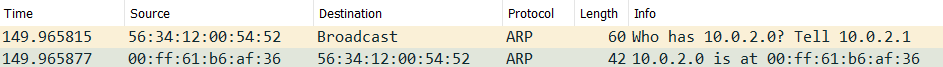
\includegraphics[scale=0.6]{images/network/arp_request.png}
    \caption{An ARP request done by the OS, observed by WireShark}
\end{figure}

\subsection{Receiving an ARP packet}

An ARP packet has the following layout:


When we receive an ARP request to our given IP, we craft a response packet with our MAC address and immediately send it back.

\begin{lstlisting}[caption={Sending back an ARP response}]
if (arp_header->ip_dst == self_ip) {
    // respond to the request
    const size_t packet_rep_size = sizeof(struct eth_hdr) + sizeof(struct arp_hdr);
    uint8_t     *packet_rep_data = malloc(packet_rep_size);
    _make_ETH_header(packet_rep_data, arp_header->eth_src, ETH_TYPE_ARP);
    _make_ARP_header(packet_rep_data + sizeof(struct eth_hdr), arp_header->eth_src,
                     arp_header->ip_src, ARP_OP_REP);
    simple_async_request(ns.async, packet_rep_data, packet_rep_size, async_request_free,
                         NULL);
}
\end{lstlisting} 

\subsection{Sending an ARP packet}

In order to send an ARP packet, we set its destination to the special MAC address FF.FF.FF.FF.FF.FF meaning we broadcast it. The request is then saved to a doubly linked list, along with the target IP. This way, when we receive an ARP response, we look at the linked list, find any request it can match and satisfy them.

\subsection{Dealing with timeouts}

Of course, if we send a request to an IP which does not exist, we will never get an answer. To deal with this, for each request, we set an associated \verb|deferred_event| which after a given time (5 seconds for an ARP request) will trigger, cause the item to be removed from the doubly linked list and a \verb|NETWORK_ERR_IP_RESOLVE_TIMEOUT| error to be returned.

\begin{lstlisting}[caption={dealing with timeouts}]
static void _network_arp_timeout(void *arg)
{
    struct request_with_timeout *req = arg;
    // remove it from the list
    req->next->prev = req->prev;
    req->prev->next = req->next;

    *req->err = NETWORK_ERR_IP_RESOLVE_TIMEOUT;
    req->resume_fn.handler(req->resume_fn.arg);
    free(req);
}
\end{lstlisting}  

This method is of course used for any request made, to make sure we are not stuck waiting for a response. If we get a response, we cancel the deferred event using \verb|deferred_event_cancel|.

\subsection{IP to MAC cache}

We want to minimize the number of requests done, as such it is inefficient to query the MAC of an IP address if we already have a way to get it. To fix this issues, the network handler has an IP to MAC cache.
\begin{lstlisting}
// hash table containing the ip to mac addresses we received
collections_hash_table *ip_to_mac;
\end{lstlisting}
This cache is done using a hash table. An IP can be represented as a 32-bit integer and is the key in this hash table to find the MAC address. Every time we receive an ARP or IP packet, we get access to the IP and MAC address of the sender and store it.

\section{Ping support}

Next is the support for the ping command, this commands relies on the ICMP (Internet Control Message Protocol) packet, the client sends an echo request and the target sends a reply with data of the request to prove it received it.

\begin{figure}
    \centering
    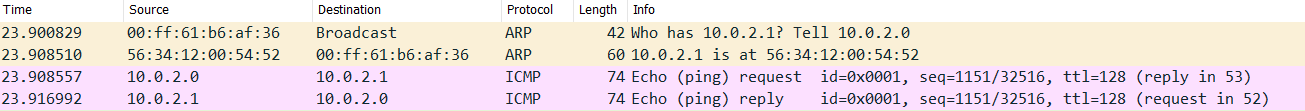
\includegraphics[scale=0.45]{images/network/ping_request.png}
    \caption{A ping request to the OS, observed by WireShark}
\end{figure}

\subsection{Receiving a ping request}

When we receive a PING request, we can immediately reply to it. The ICMP packet (and the above IP packet) are more complex, they require a checksum to check the integrity of the packet, which is the bitwise not of the added 16-bit values of the packet with carry.

An ICMP packet also has two identifiers and a payload which we need to send back to prove that we have correctly received the packet.

\begin{lstlisting}[caption={Replying to an ICMP packet}]
const uint16_t ip_packet_res_size    = sizeof(struct ip_hdr) + packet_size;
const uint16_t total_packet_res_size = sizeof(struct eth_hdr) + ip_packet_res_size;
uint8_t       *res_packet            = malloc(total_packet_res_size);
_make_ETH_header(res_packet, src_mac, ETH_TYPE_IP);
_make_IP_header(res_packet + sizeof(struct eth_hdr), src_ip, ip_packet_res_size,
                IP_PROTO_ICMP);
_make_ICMP_header(res_packet + sizeof(struct eth_hdr) + sizeof(struct ip_hdr), packet_size,
                  icmp_header->payload, ICMP_ER, ntohs(icmp_header->id),
                  ntohs(icmp_header->seqno));
\end{lstlisting}

\subsection{Sending a ping request}

Sending a ping request is more complex as we may need to make an ARP request, it has the following scheme:
\begin{itemize}
\item Serialize the request, if we already have the MAC address, skip the next step
\item Compute the current timestamp, send an ARP request and put the request in the ARP list. If we get a timeout, return immediatly.
\item Generate the payload, send the ICMP request and put the request in the ping list.
\item If we get a timeout, return \verb|NETWORK_ERR_REQUEST_TIMEOUT|.
\item Otherwise, compute the time the ping request took and send it back.
\end{itemize}

For each new ping request, we have a different identifier and generate a different payload (containing only lowercase english characters). When we receive the request, we check that the identifier and payload matches.

\section{UDP support}

The UDP protocol is really simple, it adds a source port and destination port but is much simpler than the ICMP packet. The difficulty lies in setting an easy to use UDP server for a process.

\subsection{Interface}

The network library comes with a header \verb|network.h| in aos which can be used by any process to do network requests:
\begin{lstlisting}[caption={network.h interface}]
errval_t network_init(void);

errval_t ping(uint32_t target_ip, uint32_t* ping_ms);

errval_t network_listen(uint16_t port, enum server_protocol protocol, network_listener listener, void* meta);

errval_t network_send(uint32_t ip, uint16_t port, enum server_protocol protocol, uint16_t src_port, uint16_t data_size, void* data);
\end{lstlisting}

Network init is used to setup some internal structures which we will talk about and setup the secondary asynchronous channel if it was not already setup. 

\subsection{UDP server}

The UDP server is divided in two parts. First each process has a singly linked list containing a port and the callback to call.
\begin{lstlisting}
struct listener_list{
    struct listener_list* next;
    enum server_protocol protocol;
    uint16_t port;
    network_listener listener;
    void* meta;
};
\end{lstlisting} 

Then the init process containing the network handler has a hashmap, containing for each port the process id which is listening to it (if there is one).

\begin{lstlisting}
errval_t network_register_listen(uint16_t port, bool is_tcp, domainid_t pid){
    uint64_t key = port * 2ULL + is_tcp;
    if (collections_hash_find(ns.port_to_pid, key) != NULL)
        return NETWORK_ERR_PORT_ALREADY_USED;

    collections_hash_insert(ns.port_to_pid, key, (void*)(uint64_t)pid);

    return SYS_ERR_OK;
}
\end{lstlisting}

This way when we received a UDP request, the following happens:
\begin{itemize}
\item Look in the network handler hash table if there is a process listening to it, if not return.
\item Craft a request to the given PID, if in the same core, send it immediately using its async channel. Otherwise, send it to the appropriate core.
\item The process looks in its linked list for the callback to call given the port, then calls it.
\end{itemize}


\subsection{Remote Shell}

Using UDP packet, we can now implement a shell over the network. This remote shell is using UDP packet, meaning some packets can be lost. To do so, a new shell command \verb|setio| is added to define whether to use serial or network io. And for network io which remote ip, port and host port to use.

\medskip

The \verb|getchar| and \verb|putchar| functions are then intercepted in the RPC handler and the network version of these functions are used if enabled. We also look when receiving a UDP packet if it matches the parameters of the remote shell and if so use its content for serial io.

\begin{figure}[H]
    \centering
    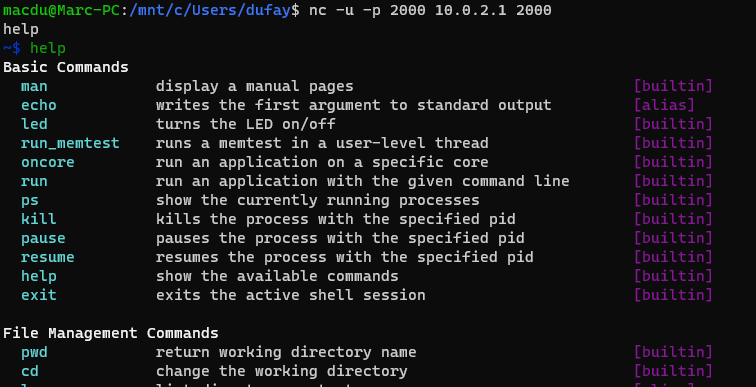
\includegraphics[scale=0.75]{images/network/network_io.png}
    \caption{Using netcat as a shell for our OS}
\end{figure}

\section{Performance}

\begin{figure}
    \centering
    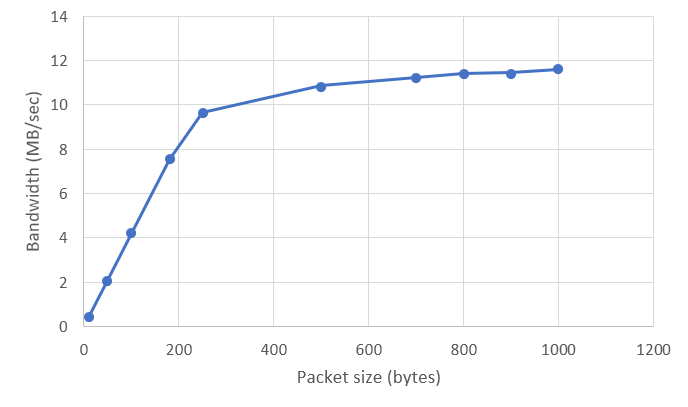
\includegraphics[scale=0.7]{images/network/graph-perf.png}
    \caption{Bandwidth recorded using the enet driver, depending on the packet size}
    \label{fig:enter-label}
\end{figure}

To test the implementation, a stress test was done by sending as many UDP packets of a given size as possible in a given time range. The UDP packet were crafted and sent by a C++ program using boost asio. When the packet is greater than 500 bytes, no packet loss was recorded. The smaller the packet was, the bigger the percentage of packet loss became, with 50\% packet loss using packets of 10 bytes.

\medskip

Furthermore, it appears that the driver has a hard limit of around 42.5 thousands packets per second, which is reached for packets of size less than 200 bytes. The maximum bandwidth recorded was almost 12 MB/sec, reached with the biggest packet size (packets bigger than 1000 bytes were getting fragmented). About latency, performing 100 ping request and taking the average, we get a value of 5ms, which means packets have a 2.5ms latency in average.

\section{Retrospective}

Networking is by nature asynchronous, which is complex to implement in an operating system with a language like C which does not allow lambda or asynchronous operators. Building an architecture that supports well this asynchronous aspect and did not block at any time was the hardest part of this milestone and took a lot of planning.

The fact that the driver does not support interrupts makes also the driver not efficient, as it must always poll for new packets in order to minimize latency.
\chapter[Distributed Capabilities]{Distributed Capabilities \\ \Large \textnormal{Georgijs Vilums}}

\label{chapter:distcap}

Throughout all of the previous chapters, we have been working under one severe limitation: Capabilities cannot be transferred between cores. However, because capabilities are so fundamental to the functioning of Barrelfish, the system cannot be considered complete without complete support for the entire set of capability operations, both on a single core and on both cores at the same time.

In this chapter, we will discuss the design decisions that went into designing our distributed capability system, the implementation hurdles we faced, how we integrated it with the system, and how we tested it.

\section{Deleting and Revoking Capabilities on a Single Core}
\label{section:distcap:dellocal}
Before we dive right into the the core of the system, let us first consider the simpler cases where we want to revoke or delete the last copy of a capability that is located only on a single core. This operation is quite simple: Because our init process is single-threaded and non-blocking, we do not actually need to worry about concurrency. Instead, we simply execute the requested operation (\texttt{monitor\_revoke\_mark\_target} for a revoke request, or \texttt{monitor\_delete\_last} for a delete request). Then, a handler is registered on the delete stepping system to send a response to the original caller once all operations have been processed.

\section{Sending Capabilities Across Cores}
Listing \ref{listing:captransfer} shows the internal interface for transferring capabilities between cores. As mentioned in section \ref{section:rpc:async}, this interface is rarely used directly, and is instead mostly an implementation detail of the \texttt{async\_channel}.

\begin{lstlisting}[caption={Internal interface for cross-core capability tranfers},label={listing:captransfer}]
struct cap_transfer {
    struct capability cap;
    coreid_t          owner;
    uint8_t           relations;
    bool valid;
};

errval_t cap_transfer_copy(struct capref cap, struct cap_transfer *transfer);
errval_t cap_transfer_move(struct capref cap, struct cap_transfer *transfer);

errval_t cap_from_transfer(struct cap_transfer *transfer, struct capref cap);
bool     cap_transfer_is_valid(struct cap_transfer *transfer);
\end{lstlisting}

\texttt{cap\_transfer\_move} and \texttt{cap\_transfer\_copy} are used to package a capability into a \texttt{struct cap\_transfer}, which can then be sent to another core. These functions both follow the same pattern:
\begin{enumerate}
    \item Populate the \texttt{cap} field with the help of \texttt{monitor\_cap\_identify}
    \item Obtain the local relations of the capability. These will become the remote relations of the capability on the other core.
    \item Set the owner. When copying, the owner remains unchanged. When moving, if there are no more local copies, the owner is set to the other core. 
    \item Update the remote relations of the capability on this core by setting the remote copy bit.
    \item If moving, nullify the capability on this core.
\end{enumerate}

Receiving the capability on the other core simply consists of using \texttt{monitor\_cap\_create} to create the capability, followed by setting the remote relations to the provided value.

As mentioned at the beginning of this section, the interface for sending capabilities between cores is mostly an implementation detail of the \texttt{async\_channel}. In fact, the only requests that use the raw interface are those made at the very beginning of system initialization, when the second core is being booted. After that point, all capability transfers are handled by the async channel: Capabilities are automatically serialized on the sending core, and re-created on the other core before the corresponding handler function runs.

This interface not only exists as a convenience factor, but also guarantees the correct operation of the distributed capability system. As an example, consider a situation where core 0 sends a request to core 1 containing a capability, and subsequently issues a revocation request for the capability contained in the request. If, for example, the request handler handling the initial request suspends before initializing the capability on the remote core, the revocation request may attempt to revoke a capability which does not (yet) exist. The capability would essentially evade revocation while in a serialized form.

Handling the sending and receiving of capabilities on the level of the async channel ensures that all requests dealing with capabilities are processes exactly in the order in which they are issued, preventing the above situation from ocurring.

\section{Synchronizing Capabilty Operations}
\label{section:cap:sync}
When remote copies or descendants of a capability exist, synchronization is required to ensure that the state stays consistent. In princpile, this procedure always consists of the same steps:
\begin{enumerate}
    \item Lock the target capability. If it is already locked, wait until it is unlocked and retry.
    \item Send a synchronization request to the other core containing details about the original request.
    \item (On the other core) Perform the synchronization actions, and send a response to the original core.
    \item Unlock the target capability.
    \item Perform the requested operation.
\end{enumerate}

One communication round trip is sufficient because our system only utilizes two cores. This obviates the need for a two-phase commit, as the core receiving the synchronization message can immediately decide if the operation can be performed and perform it, without having to notify the original core in-between. This would not be possible with three or more cores, as neither of the remote cores could unilaterally decide to execute the operation without receiving a confirmation from the other cores.

\subsection{Suspensions}
As discussed in chapter \ref{chapter:mp}, in our design, the init process is single-threaded and completely asynchronous. This introduces some additional complications for the synchronizing capability operations: In contrast to other operations, which need to suspend at most once (for example, a \texttt{wait} operation only needs to suspend once and resumes once the target process exits), all of the synchronizing capability operations may need to suspend and resume at multiple points during the process (and potentially even multiple times at a single point). Because the call stack is not preserved across suspensions, all of the state necessary to process a request through its lifetime must be stored in a heap-allocated structure. An example for the delete operation (discussed later) is shown in listing \ref{listing:delsuspend}:

\begin{lstlisting}[caption={State preserved across suspension points in the delete handler},label={listing:delsuspend}]
struct delete_suspend {
    struct aos_rpc_handler_data rpc_data;
    struct delete_sync          sync;
    struct domcapref            cap;
    struct delete_queue_node    qn;
};
\end{lstlisting}

The structure contains various elements:
\begin{enumerate}
    \item The \texttt{aos\_rpc\_handler\_data} containing the state of the request, required for sending the response after the operation finishes.
    \item A \texttt{delete\_sync} object, which is sent to the other core for synchronization (discussed later).
    \item A reference to the capability being delete.
    \item The queue node for waiting for the delete stepping framework.
\end{enumerate}
Similar structures exist for revocations and retype operations.

\subsection{Waiting for a Lock}
All of the synchronizing capability operations lock the capability before performing any remote synchronization. Because a capability may already be locked when a request arrives and init must be nonblocking, it may be necessary to suspend until the capability is unlocked. This is achieved through using the provided facilities for waiting on a locked capability (\texttt{caplock\_wait}), and performing notifying unlocks. Listing \ref{listing:deletelock} shows this process for the \texttt{delete} operation. It first attempts to lock the capability. If the capability is locked, a callback to the \textit{same function} is registered, to be executed once the capability is unlocked. Notice that by the time the callback is executed, the capability may have been locked again. Hence, this function may suspend an arbitrary number of times at the same point (although this is highly unlikely).

Once the lock on the capability has been acquired, the cross-core synchronization process begins.

\begin{lstlisting}[caption={Waiting for a lock before beginning the capability deletion process},label={listing:deletelock}]
static void delete_step_1(void* arg) {
    struct delete_suspend *suspend = arg;
    errval_t err = monitor_domcap_lock_cap(suspend->cap);
    if (err_no(err) == SYS_ERR_CAP_LOCKED) {
        caplock_wait(suspend->cap, &suspend->qn.qn, MKCLOSURE(delete_step_1, suspend));
    } else if(err_is_ok(err)) {
        /* continue with cross-core sync */
    } else {
        USER_PANIC_ERR(err, "monitor_domcap_lock_cap");
    }
}
\end{lstlisting}

\subsection{Remote Delete}
The first operation with remote synchronization which we will consider is the deletion of the last copy of a capability when remote copies exist. The procedure is very similar to the general process described at the beginning of this section. There are three cases which need to be handled:
\begin{enumerate}
    \item The current core is the owner, and the capability is moveable. In this case, ownership is transferred to the other core.
    \item The current core is the owner, and the capability is not moveable. This means that all remote copies need to be deleted.
    \item The other core is the owner. We only need to message it to update its remote relations for the capability being delete (i.e. unset the remote copy bit).
\end{enumerate}
The correct case is chosen based on the results of \texttt{monitor\_get\_domcap\_owner} and \texttt{distcap\_is\_moveable}. Based on this, the structure shown in listing \ref{listing:deletesync} is populated and sent to the other core through an asynchronous request.

\begin{lstlisting}[caption={Synchronization message for the delete operation},label={listing:deletesync}]
struct delete_sync {
    struct aos_distcap_base_request base;
    struct capability               cap;
    uint8_t                         owner;
    enum {
        DELETE_SYNC_MOVE_OWNER,
        DELETE_SYNC_DELETE_FOREIGNS,
        DELETE_SYNC_LAST_NONOWNER,
    } op;
};
\end{lstlisting}

Upon receiving this message, the other core needs perform an operation depending on the \texttt{op} specified in the message. The process is illustrated in in listing \ref{listing:deletesyncremote}\footnote{The listing is simplified to make it more readable.}: First, a temporary copy of the target capability is created, to create a target on which the capability operations can be executed on. Next, depending on the \texttt{op} field, one of three operations is performed, as described at the beginning of this section:
\begin{enumerate}
    \item To move ownership to this core, \texttt{monitor\_set\_cap\_owner} is used.
    \item All foreign copies are deleted using \texttt{monitor\_delete\_foreign}.
    \item The remote copy bit is unset using \texttt{monitor\_remote\_relations}.
\end{enumerate}
After the operation is executed, the temporary copy of the capability is nullified. It is only an artifact of implementing the necessary operations, and must not remain on the core.

\begin{lstlisting}[caption={Case distinction for delete synchronization operation},label={listing:deletesyncremote}]

monitor_cap_create(tempcap, &sync->cap, owner);
if (sync->op == DELETE_SYNC_MOVE_OWNER) {
    // set the owner of the cap to this core
    monitor_set_cap_owner(cap_root, get_cap_addr(tempcap), 
        get_cap_level(tempcap), disp_get_core_id());
} else if (sync->op == DELETE_SYNC_DELETE_FOREIGNS) {
    // delete all copies of the cap on this core
    monitor_delete_foreigns(tempcap);
} else if (sync->op == DELETE_SYNC_LAST_NONOWNER) {
    // unset RRELS_COPY_BIT
    monitor_remote_relations(tempcap, 0, RRELS_COPY_BIT, NULL);
} else {
    USER_PANIC("Unknown delete sync operation");
}
monitor_nullify_cap(tempcap);
\end{lstlisting}

Finally, after the operations on the remote core are executed and the sending core receives a response, the final step of the operation can be executed, again depending on the \texttt{op} field. The process is shown in listing \ref{listing:deletefinal}. In the case of deleting the last copy of a capability when the other core is already the owner or could be made the owner, we simply nullify the local copy of the capability. No cleanup must be performed, because that will occur once the capability is deleted on the other core. If, on the other hand, the capability could not be moved, we need to now delete the last local copy with the help of the delete stepping framework. At this point, no more remote copies exist, hence the process is the exact same as for deleting local capabilities, described in section \ref{section:distcap:dellocal}.

\begin{lstlisting}[caption={Final step of synchronized delete},label={listing:deletefinal}]
struct domcapref cap = suspend->cap;
// we locked the cap before sending the remote request. unlock it now
caplock_unlock(cap);
if (suspend->sync.op == DELETE_SYNC_LAST_NONOWNER 
    || suspend->sync.op == DELETE_SYNC_MOVE_OWNER) {
    // Capability (now) lives on the other core. Nullify the remaining local copy
    monitor_nullify_domcap(cap.croot, cap.cptr, cap.level);
    // send the response to original caller
    suspend->rpc_data.resume_fn.handler(suspend->rpc_data.resume_fn.arg);
    free(suspend);
} else if (suspend->sync.op == DELETE_SYNC_DELETE_FOREIGNS) {
    // all foreign copies were deleted. now delete local copies and register response callback
    delete_last(cap);
    delete_queue_wait(&suspend->qn, MKCLOSURE(queue_delete_handler, suspend));
} else {
    USER_PANIC("invalid delete sync op");
}
\end{lstlisting}

\subsection{Remote Revoke}
Even though a capability revocation is a much more involved process than a simple deletion, the synchronization process is actually simpler, because there are less distinct cases to handle. Fundamentally, the same operation needs to happen on all cores: Mark all copies and descendants of the target capability, and then run the delete stepping framework until completion. The only reason why there even are multiple cases is because a different operation must be executed depending on whether the core is the owner of the target capability or not.

Similarly to a remote deletion, the process begins by locking the capability and filling an instance of \texttt{struct revoke\_sync}, shown in listing \ref{listing:revokesync}, with relevant data about the target capability.

\begin{lstlisting}[caption={Payload for revoke synchronization},label={listing:revokesync}]
struct revoke_sync {
    struct aos_distcap_base_request base;
    capability_t                    cap;
    uint8_t                         owner;
};
\end{lstlisting}

After receiving the synchronization message, the remote core must execute one of two different marking operations, depending on whether it is the owner of the capability that is being revoked. If it isn't, \texttt{monitor\_revoke\_mark\_relations} can be used directly on the \texttt{struct capability} that was passed in the sync message. Otherwise, a temporary copy of the capability must be created and marked with \texttt{monitor\_revoke\_mark\_target}, and subsequently nullified. 

After marking, the remote core waits for the delete queue to empty, and subsequently sends a response. Then, the core issuing the original request must perform the same procedure: If it is the owner of the capability, \texttt{monitor\_revoke\_mark\_target} is used (creating a temporary copy is not necessary, as the capability is already present on the requesting core). If the other core owns the capability, \texttt{monitor\_revoke\_mark\_relations} is used. After the delete queue empties, the response to the original request is sent.

\subsection{Remote Retype}
The remote retype is actually the simplest operation in terms of synchronization. The general flow is, again, very similar to the other operations: We first attempt to lock the capability (and if we can't, suspend until we can). Next, we check if we can perform the retype locally, as there is no need to synchronize if the operation is invalid anyway. 
Next, a synchronization message (shown in listing \ref{listing:retypesync}) is sent to the other core. The other core checks the contents of this message to decide whether the retype operation should be allowed, using \texttt{monitor\_is\_retypeable}. If the check succeeds, it also immediately updates the remote relations of its local copy of the retyped capability to set the descendant bit\footnote{For this, it is necessary to create a temporary local copy}. This is important to ensure that a future revoke of the capability would also clean up children on the other core. Once the confirmation arrives from the other core, the retype is performed and a response is sent.

\begin{lstlisting}[caption={Payload for retype synchronization},label={listing:retypesync}]
struct retype_sync {
    struct aos_distcap_base_request base;
    capability_t                    cap;
    uint8_t                         owner;
    gensize_t                       offset;
    gensize_t                       objsize;
    size_t                          count;
};
\end{lstlisting}

While implementing the remote retyping operation, we actually came across a bug in the kernel. As shown in listing \ref{listing:retypebug}, the system call arguments for the capability source pointer are mixed up, and the value of \texttt{offset} is passed as the address of \texttt{src}. As the kernel later accesses \texttt{src}, a kernel panic occurs.

\begin{lstlisting}[caption={Bug in the invocation handler for \texttt{monitor\_is\_retypeable}},label={listing:retypebug}]
INVOCATION_HANDLER(monitor_handle_is_retypeable)
{
    (void)kernel_cap;
    INVOCATION_PRELUDE(5);
    // check access to user pointer
    if (!access_ok(
        ACCESS_READ, sa->arg1, sizeof(struct capability))) {
        return SYSRET(SYS_ERR_INVALID_USER_BUFFER);
    }

    struct capability *src = 
        (struct capability *)sa->arg2; // should be sa->arg1

    uintptr_t offset  = sa->arg2;
    uintptr_t objsize = sa->arg3;
    uintptr_t count   = sa->arg4;

    return sys_monitor_is_retypeable(
        src, offset, objsize, count);
}
\end{lstlisting}

Furthermore, we also came across a bug in the provided \texttt{distops} implementation. Listing \ref{listing:retypebug2} shows the provided implementation of \texttt{monitor\_domcap\_retype\_remote\_cap}. It wrongly uses \texttt{get\_croot\_addr} instead of \texttt{get\_cap\_addr} to get the addresses of capabilities referring to the CSpace roots of the capabilities to be retyped. This leads to the wrong slots being looked up by the kernel and prevents the retype operation from functioning correctly.

\begin{lstlisting}[caption={Bug in the invocation code for retyping a \texttt{domcap}},label={listing:retypebug2}]
errval_t monitor_domcap_retype_remote_cap(
    struct domcapref dest_start, 
    struct domcapref src, 
    gensize_t offset, 
    enum objtype newtype, 
    gensize_t objsize, 
    gensize_t count, 
    capaddr_t slot
) {
    return invoke_monitor_remote_cap_retype(
        get_croot_addr(src.croot), // should be get_cap_addr
        src.cptr, 
        offset, 
        newtype, 
        objsize, 
        count, 
        get_croot_addr(dest_start.croot), // should be get_cap_addr
        dest_start.cptr, 
        slot, 
        dest_start.level
    );
}
\end{lstlisting}

The fixes to both of these problems are deployed in our version of Barrelfish.

\section{System Integration}
As previously discussed, support for sending capabilities between cores is introduced completely transparently by the asynchronous channel between each core's init process. Hence, system integration is rather easy in most places: Operations can simply be forwarded between cores, and don't have to care whether they send any capabilities or not. In this section, we will discuss the most important operations enabled by the distributed capability system, as well as operations which could be enabled in the future.

\subsection{Spawning with Capabilities}
Spawning a process with capabilities on an arbitrary core is perhaps the most important feature that is enabled by the extended capability system. And, notably, no additional implementation was required to support this functionality: Because the capability transfer is fully integrated in the async channel, spawn requests can be forwarded to the other core in the same way as previously, only that now capabilities will also be sent along (previously, the async channel would simply drop any capabilities sent with a message).

A feature which depends on this functionality is the ability to pipe data between processes on different cores: As discussed in chapter \ref{chapter:shell}, data piping is supported through a UMP frame shared between the piped processes. If the processes reside on different cores, the frame must be sent between cores to enable the piping.

\subsection{Single Memory Server}
We implement a simple form of using a single memory server: All memory requests originating from user processes running on the second core are forwarded to the main core. The mechanism through which this is achieved is completely analogous to the extended support for spawning remote processes with capabilities: The capability is simply sent along in the async channel.

A notable limitation is that this only applies to user processes: The init process still uses its statically assigned memory pool to allocate memory. This is because allocating memory from the other core requires suspending (as init is non-blocking and the other core may take arbitrarily long to serve the request), and, due to the lack of language support, it would be infeasible to incorporate suspension into all places where memory is allocated in init.

\section{Testing}
We test our distributed capability system with a user process called \texttt{tester}. The tester executes various capability operations and verifies that the correct results are obtained.

The most basic tests are only run in the main process. They test for the correct operation of the delete stepping framework, by creating a capability with local copies, and then deleting and/or revoking it. Then, by using \texttt{cap\_direct\_identify}, we verify that the target capabilities have indeed been deleted.

A set of more complex tests verifies cross-core operations. For this, we set up a set of capabilities, and then spawn the same \texttt{tester} process on the other core, sending along the capabilities we just created. We will refer to the spawning process as the parent, and to the spawned process as the child). First, the child executes the same single-process tests that the parent goes through. Then, the parent and the child perform a set of operations on their shared capabilities:
\begin{itemize}
    \item Delete a frame from the parent. The frame should remaing accessible at the child, as ownership is moved.
    \item Delete an L2 CNode from the parent. The child should not be able to access the CNode anymore, as ownership of CNodes cannot be moved.
    \item Revoke a frame from the child. The frame should become inaccessible on both the child and the parent.
    \item Revoke a RAM capability from the child, where the RAM capability has a descendant frame on the parent core. The descendant should be deleted.
    \item Retype a RAM capability from the child, where an overlapping descendant exists on the parent. This should fail.
    \item Retype a RAM capability from the child, without any overlaps. This should succeed.
\end{itemize}
If all of these operations succeed, the tests are considered a success.

\section{Retrospective}
Our decision to make the init process fully asynchronous and definitely had a big impact on how the distributed capability system had to be designed. Because some of the operations need to suspend multiple times, state management becomes convoluted and hard to follow. 

It also significantly complicates the process of performing potentially blocking capability operations from within init. A \texttt{cap\_delete} may block the process, and so would require a suspension if used from within init. However, introducing suspensions throughout the code in init would be infeasible, and hence these operations are simply not supported.

If our design instead used threads to handle incoming requests, blocking would not be an issue, and the process of waiting for a lock, sending a request, waiting for a response, and sending the response to the original request could happen from within a single function invocation.

As mentioned in prior sections, better language-level support for asynchronous programming would also be a solution.
 
\begingroup
\renewcommand\thechapter{A}
{\normalfont\huge\bfseries}{}{}{\Huge}
\chapter{Appendix}
\section{Command Line Utilities} \label{sec:appendix_user_guide}

The provided shell supports a variety of built-in commands. The \texttt{help} built-in provides a great starting point for exploring this functionality. We outline the provided functionality in Listing \ref{listing:app_help}.
 % \renewcommand{\ttdefault}{pcr}
\begin{lstlisting}[style=ShellInputStyle, deletekeywords={run, command, wc, echo, builtin, alias, return, in, ps, kill, help, exit, pwd, cd, cat, tee, time, false, true, test, set}, basicstyle=\tiny\ttfamily\color{shell_default}, label={listing:app_help}, caption={The \texttt{help} built-in provides a list of available commands}]
 +~$+ !help!
 Basic Commands
   §man§            display a manual pages                               @[builtin]@
   §echo§           writes the first argument to standard output         @[alias]@
   §led§            turns the LED on/off                                 @[builtin]@
   §run_memtest§    runs a memtest in a user-level thread                @[builtin]@
   §oncore§         run an application on a specific core                @[builtin]@
   §run§            run an application with the given command line       @[builtin]@
   §ps§             show the currently running processes                 @[builtin]@
   §kill§           kills the process with the specified pid             @[builtin]@
   §pause§          pauses the process with the specified pid            @[builtin]@
   §resume§         resumes the process with the specified pid           @[builtin]@
   §help§           show the available commands                          @[builtin]@
   §exit§           exits the active shell session                       @[builtin]@
 File Management Commands
   §pwd§            return working directory name                        @[builtin]@
   §cd§             change the working directory                         @[builtin]@
   §ls§             list directory contents                              @[alias]@
   §cat§            concatenate and print files                          @[alias]@
   §tee§            duplicate standard input                             @[alias]@
   §mkdir§          make directories                                     @[builtin]@
   §rmdir§          remove directories                                   @[builtin]@
   §rm§             remove directory entries                             @[builtin]@
Network Commands
  §ping§           ping IP address                                       @[alias]@
  §send§           send UDP packet                                       @[builtin]@
  §listen§         listen on some port                                   @[alias]@
  §setio§          set io method                                         @[builtin]@
 Utility Commands
   §time§           measures the time taken to execute another command   @[builtin]@
   §clear§          clears the screen                                    @[builtin]@
   §reboot§         reboots the system                                   @[builtin]@
   §false§          returns EXIT_FAILURE                                 @[builtin]@
   §true§           returns EXIT_SUCCESS                                 @[builtin]@
   §test§           run the specified tests in user-level                @[builtin]@
\end{lstlisting}

In particular, help conveniently indicates whether a specific command is an alias or a builtin. Beyond the \texttt{help} command, the \texttt{man} built-in provides a more detailed description for a specific command:
\begin{lstlisting}[style=ShellInputStyle, deletekeywords={run, command, wc, echo, builtin, alias, return, in, ps, kill, help, exit, pwd, cd, cat, tee, time, false, true, test, for}, basicstyle=\tiny\ttfamily\color{shell_default}]
 +~$+ !man! echo
+ NAME+
     echo - writes the first argument to standard output

+ USAGE+
     echo <message>

+ DESCRIPTION+
     prints the provided <message> to stdout.
     NOTE: `echo` only accepts a single argument (use quotes for a %*\shellrawquote*message with spaces%*\shellrawquote*).
\end{lstlisting}

\endgroup

\begingroup
\renewcommand\thechapter{B}
{\normalfont\huge\bfseries}{}{}{\Huge}

\chapter{Speed measurements}

\section{Measuring rpc}

Figures \ref{fig:b1} and \ref{fig:b2} illustrate two main observations. First, when sending a request through RPC (remote procedure call), it is generally reliable and consistent. We observe that the amount of time taken for an RPC request follows a normal distribution. However, upon closer examination, we can also identify some outliers in the computational process. These outliers can occur due to various reasons, such as a page fault that requires additional memory for the slab allocator.

Additionally, during our measurements, we noticed that sending requests after a warm-up period tends to be slightly faster. This observation is logical because it allows us to benefit from local temporal and spatial locality in the cache and the TLB (translation lookaside buffer).

\begin{figure}[htp]
    \centering
    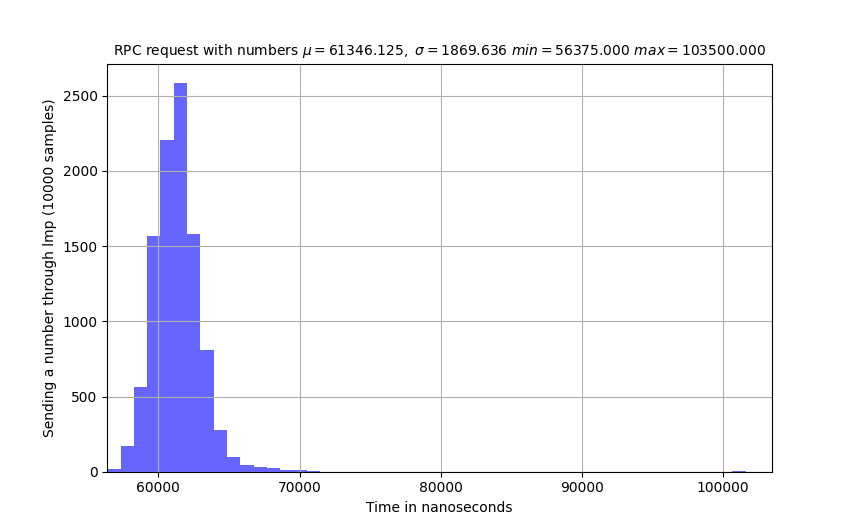
\includegraphics[width=12cm]{images/benchmarks/send_number.png}
    \caption{Latency to send a number over rpc}
    \label{fig:b1}
\end{figure}


\begin{figure}[htp]
    \centering
    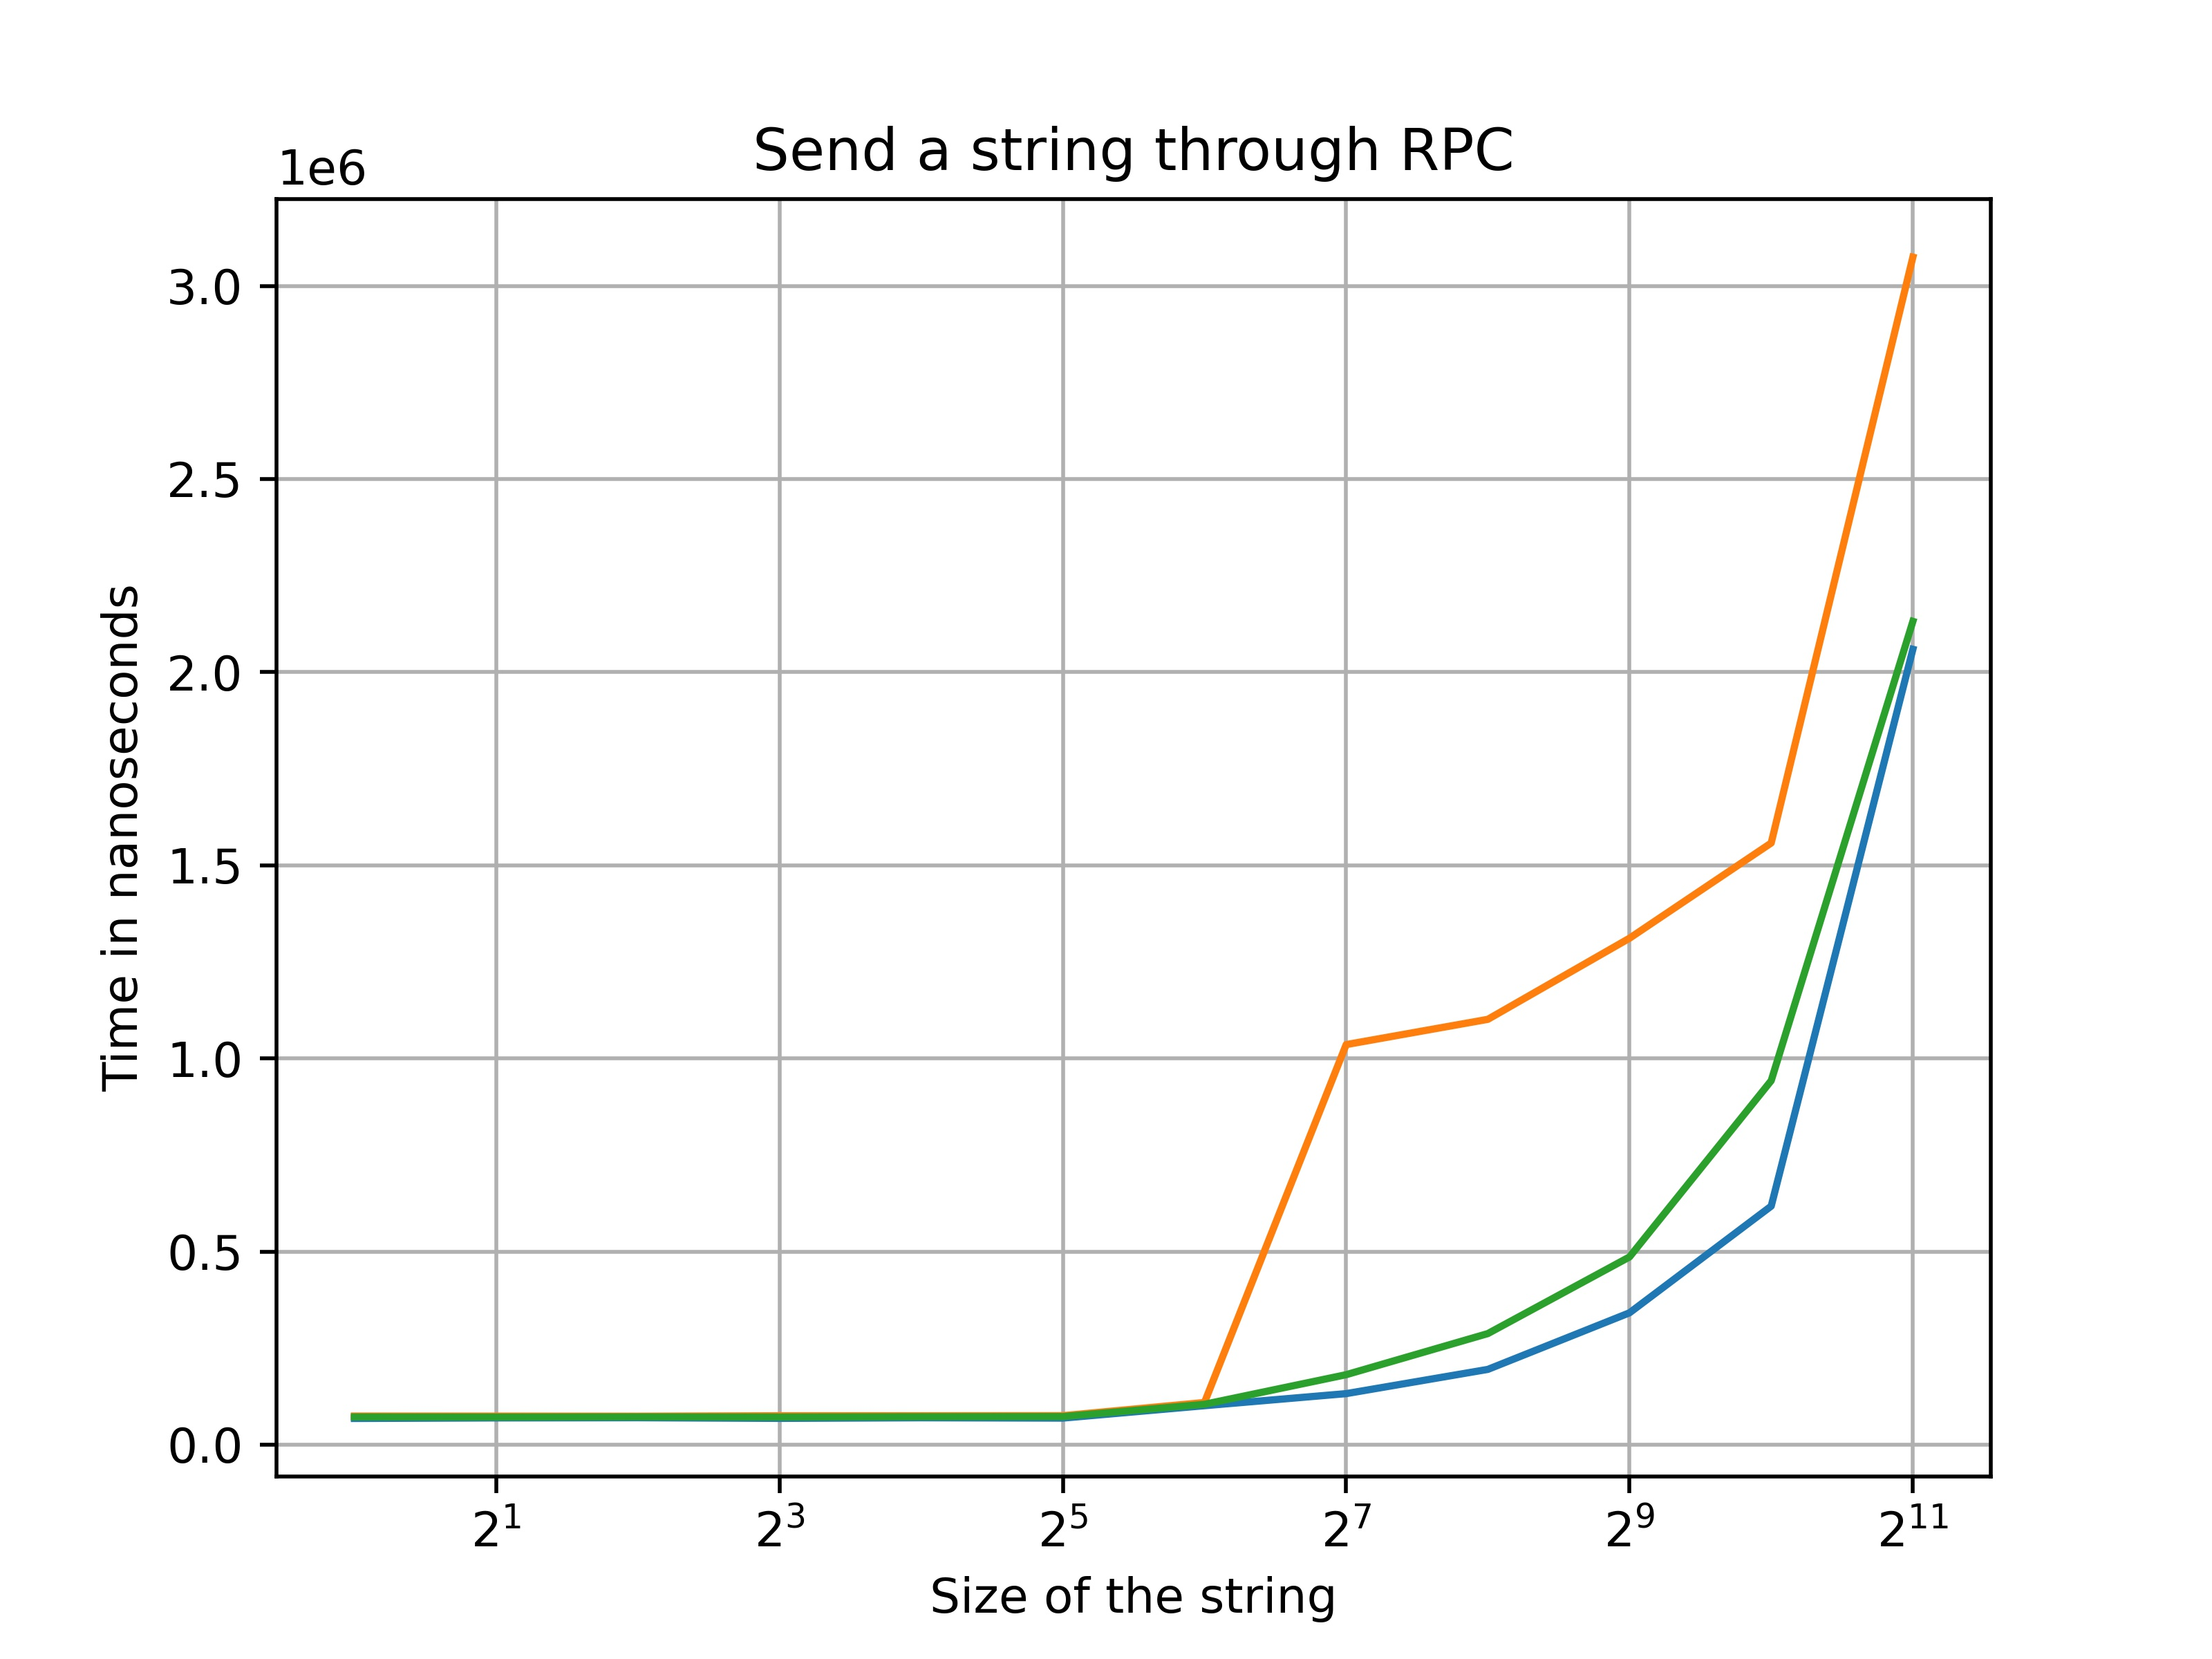
\includegraphics[width=12cm]{images/benchmarks/send_string.jpg}
    \caption{Latency to send a string over rpc}
    \label{fig:b2}
\end{figure}


\section{Measuring the physical memory allocator}

In this performance measurement, we are allocating 2560 pages of physical address without freeing any resource. The results clearly indicate that the performance gradually deteriorates over time. This decline in performance can be attributed to the necessity of traversing a linked list, which inherently takes a considerable amount of time. It is worth noting that these measurements are conducted on a newly initialized data structure, representing the optimal performance scenario. If we were to measure the performance when the data structure is not fresh, it would inevitably take more time as the performance worsens over time.

\begin{figure}[htp]
    \centering
    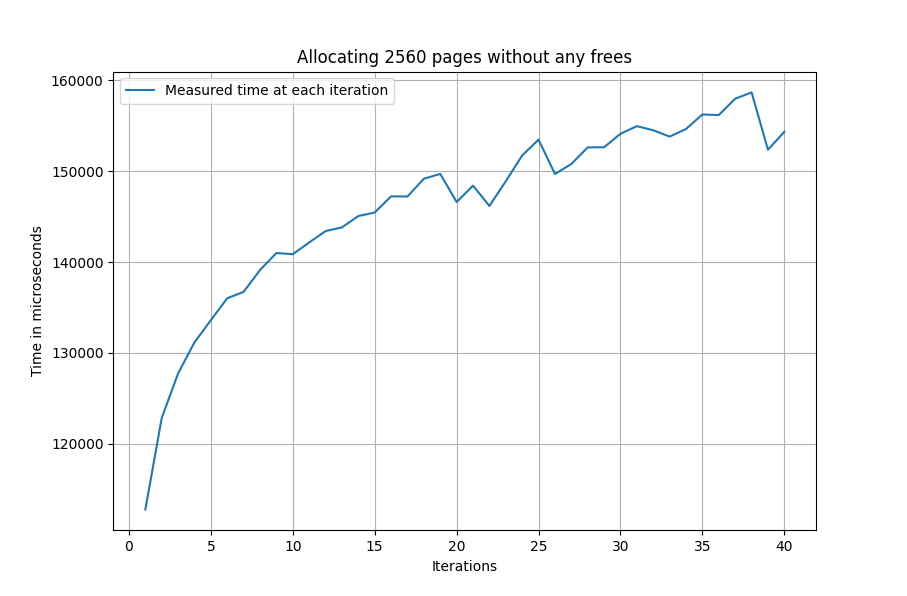
\includegraphics[width=12cm]{images/benchmarks/physical_allocator.png}
    \caption{Allocating multiple frames on the physical allocator}
    \label{fig:galaxy}
\end{figure}

\section{Measuring the virtual memory allocator}

In this  performance measurement, our focus lies on the allocation of virtual memory and the mapping of pages. It is crucial to note that in this particular benchmark, there is no actual measurement of physical allocation involved. Moreover, it is worth highlighting that our performance testing is conducted on a freshly established data structure. Just like in cases where physical memory is allocated, we observe a decline in performance as time progresses.

\begin{figure}[htp]
    \centering
    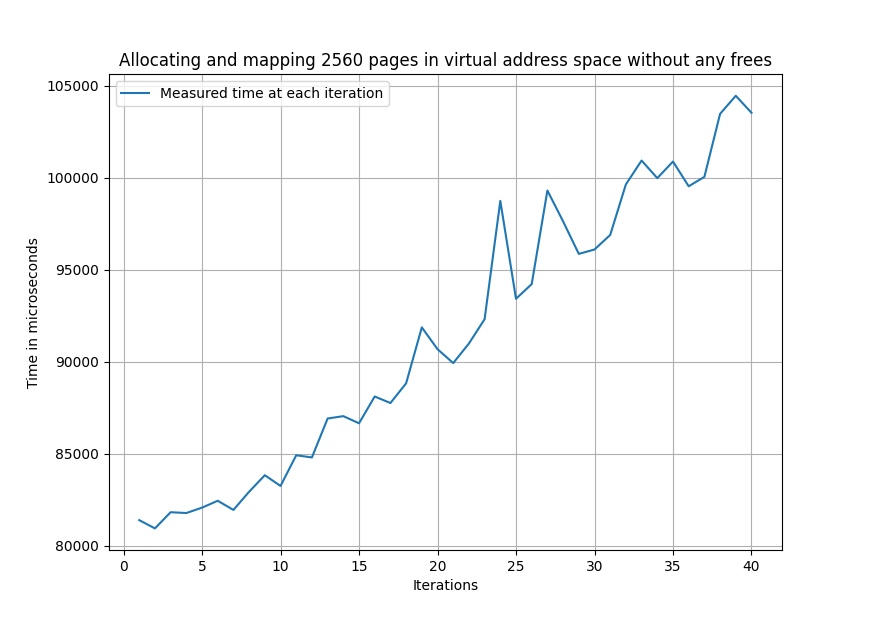
\includegraphics[width=12cm]{images/benchmarks/better.png}
    \caption{Allocating and mapping multiple frames on the virtual memory allocator}
    \label{fig:galaxy}
\end{figure}

\endgroup

\begingroup
\renewcommand\thechapter{C}
\chapter{Feedback}
{\normalfont\huge\bfseries}{}{}{\Huge}

The course was undeniably captivating and held our keen interest throughout its duration. We had the opportunity of delving into the intricate workings of operating systems and gained extensive knowledge in the process. Implementing an operating system from scratch provided us with a unique opportunity to comprehend its inner mechanisms. We encountered numerous trade-offs that necessitated careful consideration and decision-making. Furthermore, debugging proved to be more challenging in comparison to working on a single program.

\medskip

Another noteworthy positive aspect of the course that greatly enhanced our learning experience was working using a non-Unix kernel. This distinctive feature presented us with a valuable opportunity to engage in critical thinking regarding operating system designs. If we had been exposed only to a Unix-style operating system, the situation would likely have been quite different.
 
\medskip

On the whole, we express our heartfelt appreciation to the staff who orchestrated the course. The good organization ensured a smooth learning experience, and their regular presence and support on Moodle promptly addressed any concerns or difficulties we encountered.

\medskip

Nevertheless, one aspect of the course that warrants discussion is the workload. It is probably a recurring critique, but we feel compelled to highlight that the course's credit value of seven does not adequately reflect its intensity. Striking a balance between this course and our other academic commitments proved exceedingly hard, which is unfortunate. It is our belief that the course would be better served by being allocated 10-15 credits, as it would afford us more time to resolve bugs and align better with the significant investment of effort expected from students.

\endgroup

\end{document}